\chapter{Event selection and signal regions definitions}
\label{ch:evt_selection}
\epigraph{\emph{“Champions keep playing until they get it right.”}}{Billie Jean King}

The photon+jet high-mass final state represents an ideal scenario for searches of physics \ac{BSM}. As mentioned in \Ch{\ref{ch:strategy}}, bumps on the \myj distribution over the \ac{SM} are searched for by modeling the background with a functional form. In order to be able to visualise, in case of it exists, any signal (physics \ac{BSM}) over the background, it is indispensable to have an excellent knowledge of it, and to be able to separate correctly both.

Unlike count-searches, where one needs to define signal, validation and control regions to estimate the background, in resonance searches it is usual to design a signal region that is able to provide a smooth background, but also, a clean signal over it. In this chapter, all the event selection that leads to the signal regions used in this analysis are presented. In \Ch{\ref{ch:bkg}}, the estimation and modeling of the background are explained in detail.


\section{Trigger}
\label{sec:evt_selection:trigger}

Events are collected by a single photon trigger (\texttt{HLT\_g140\_loose}) with a transverse momentum treshold of \(140~\gev\) which is the lowest unprescaled photon trigger for the most part of the data taking periods\footnote{For 2015 the lowest unprescaled trigger was the \texttt{HLT\_g120\_loose}, but the \texttt{HLT\_g140\_loose} was also in the menu}, selecting events with at least one photon passing the loose identification criteria. This trigger has been kept unprescaled and is fully efficient for photons with \(145~\gev\) with uncertainties less than \(0.1\%\) above \(150~\gev\). It has been computed with a bootstrap method following the prescriptions in \cite{ATLAS-PhotonTrigger-Performance-2015} and it is shown in Figure \ref{fig:evt_selection:trigger:trigger_perf_15_18} as a function of photon \(\pt\), \(\eta\) and \(\avgmu\) for the different years of data taking.

\begin{figure}[ht!]
    \centering
    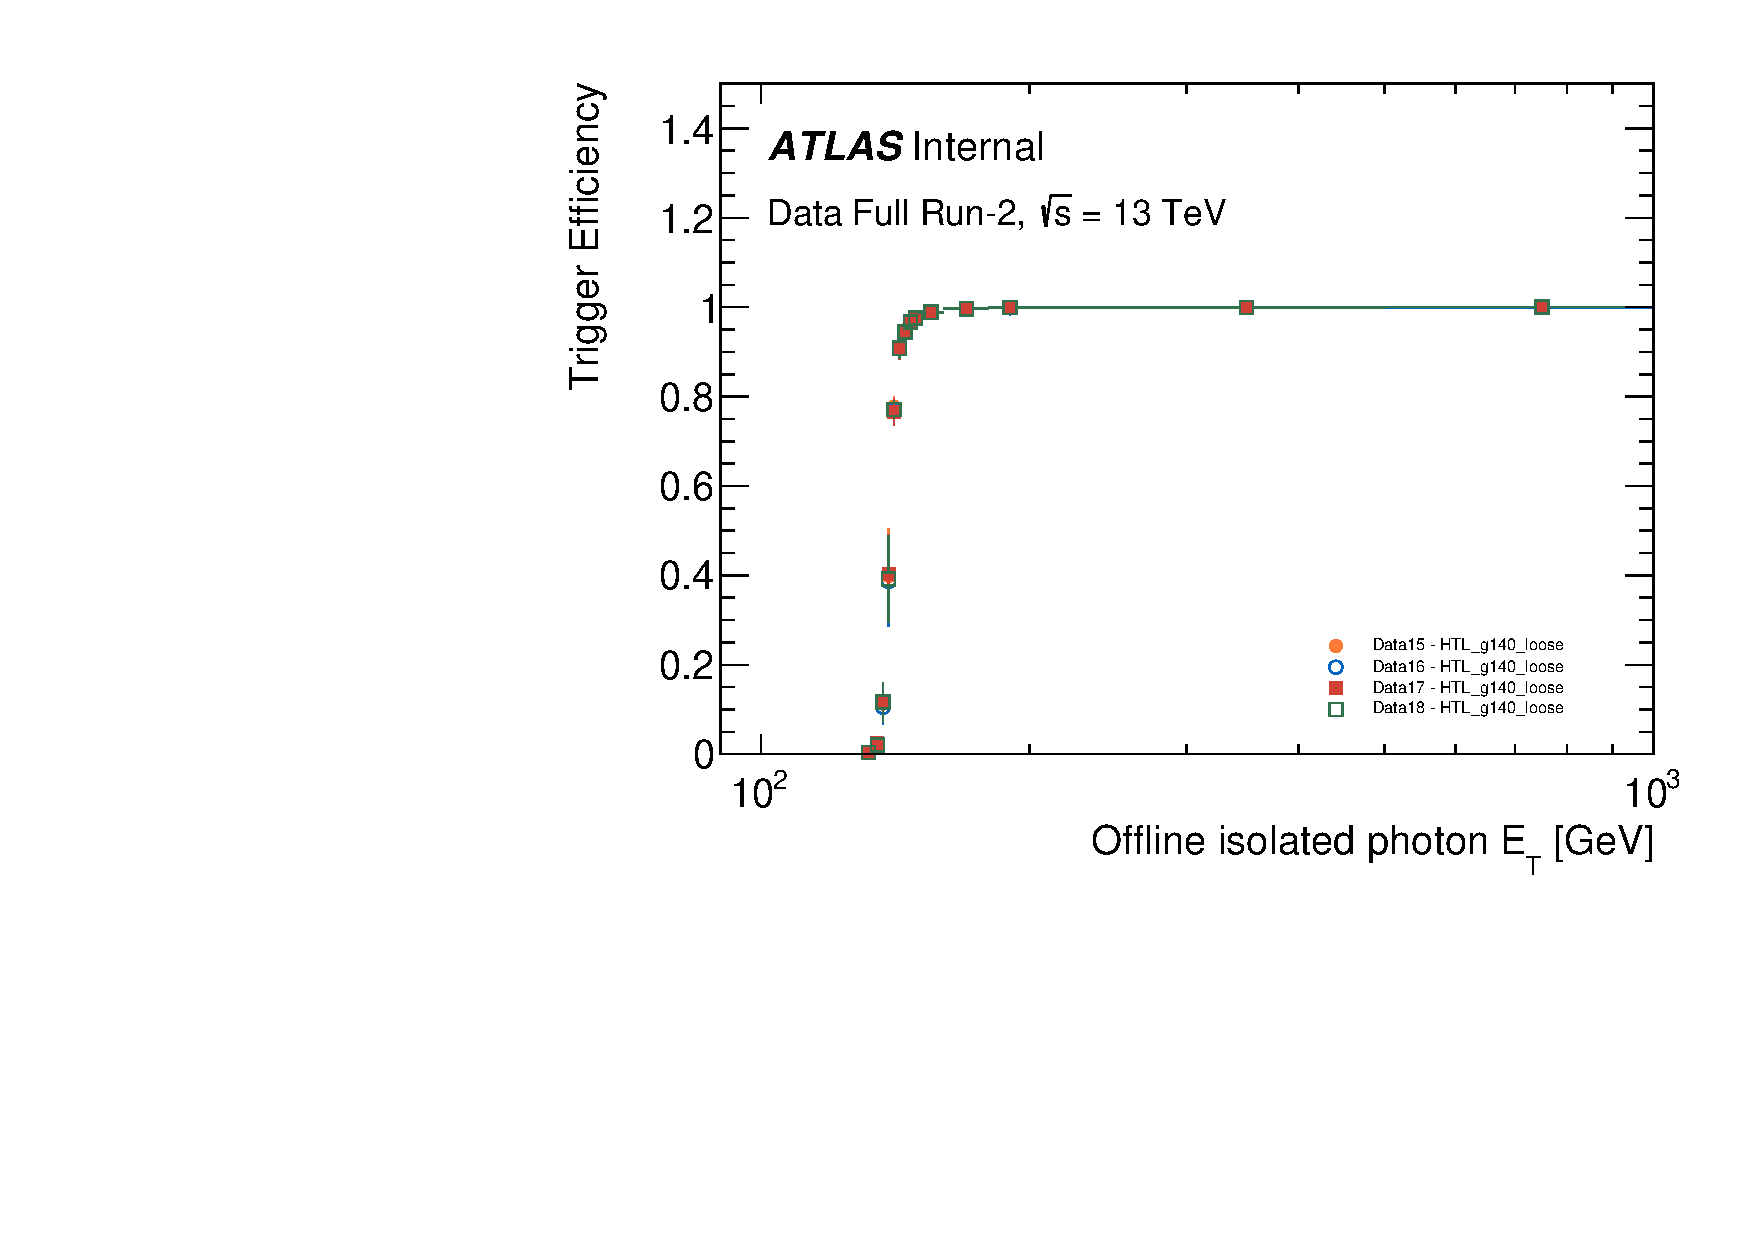
\includegraphics[width=0.32\textwidth]{5_resonances/event_selection/trigger/perfPlots_2015-2018_thesis_DATA_Et_g140_loose}
    \includegraphics[width=0.32\textwidth]{5_resonances/event_selection/trigger/perfPlots_2015-2018_thesis_DATA_eta_g140_loose}
    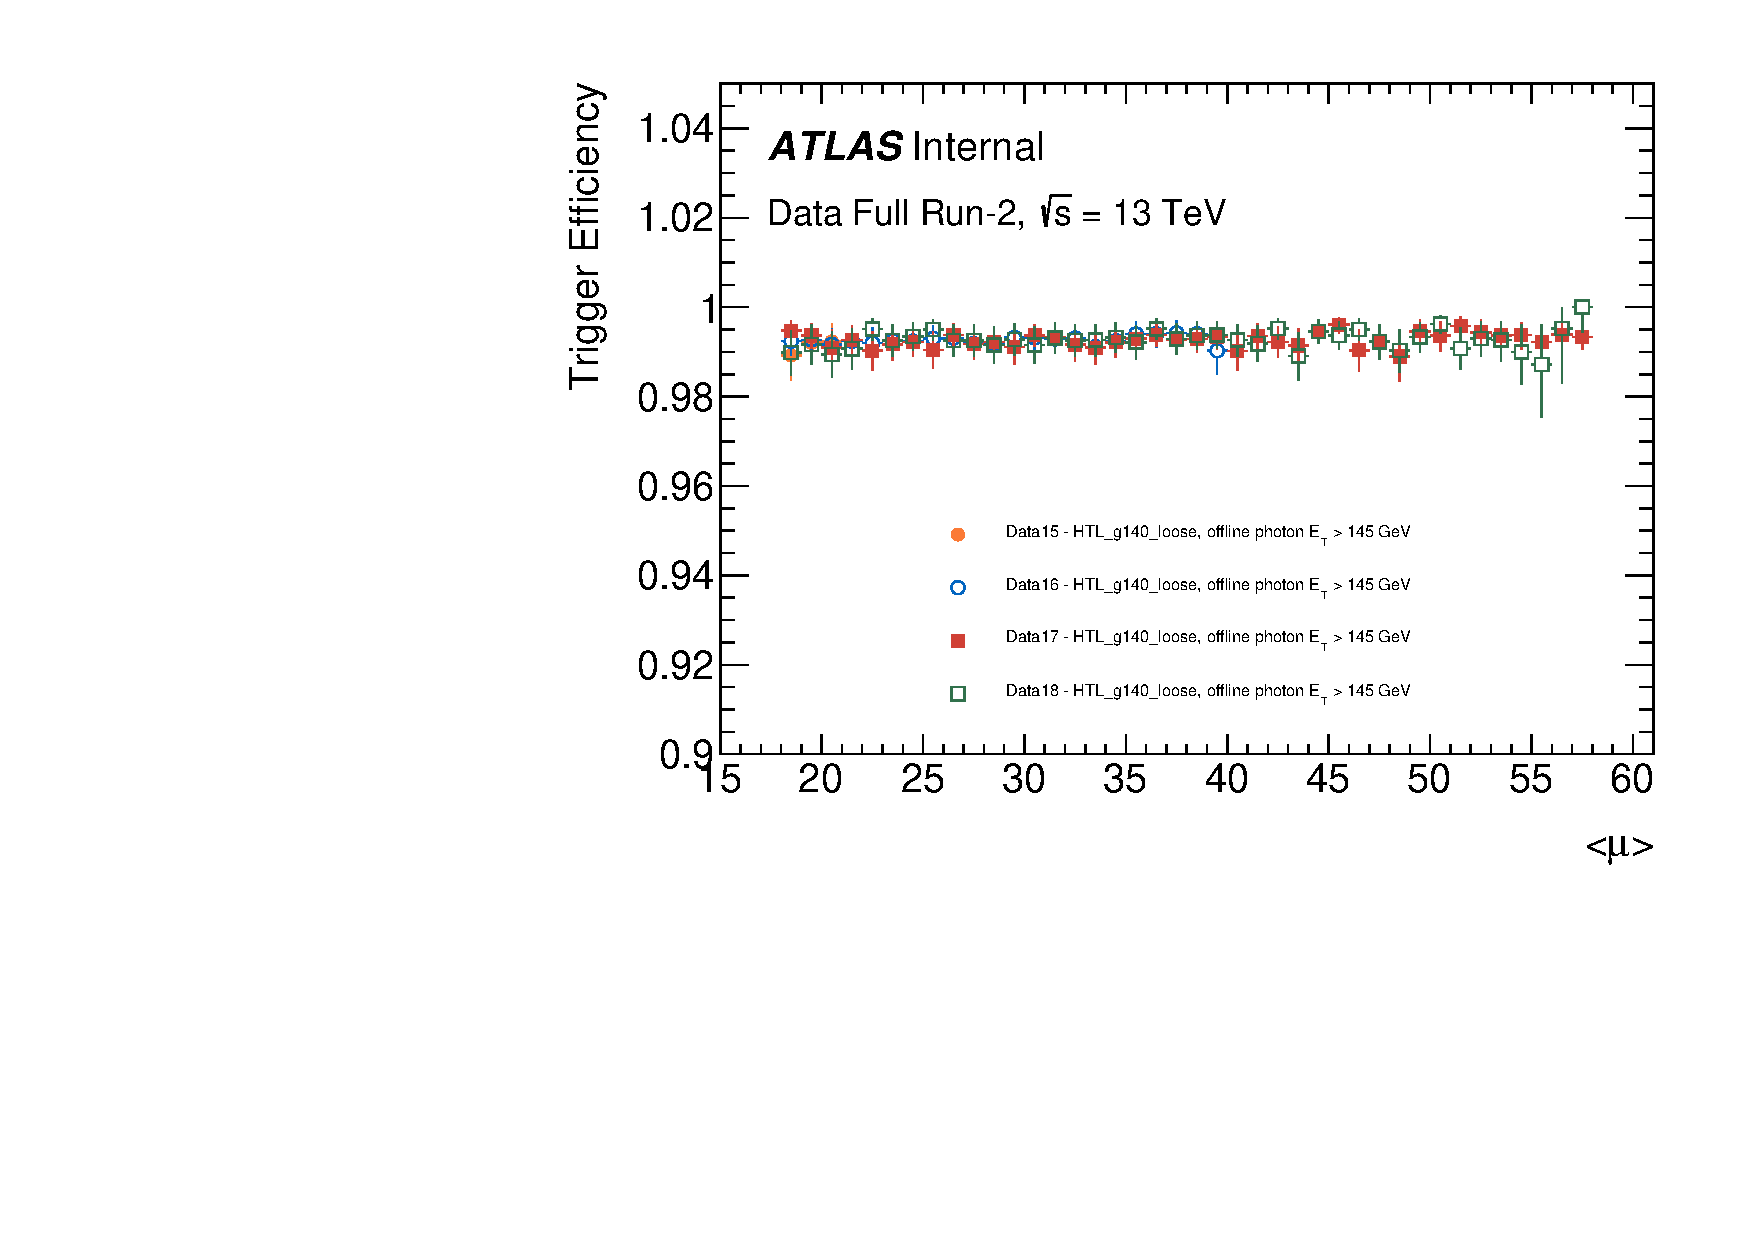
\includegraphics[width=0.32\textwidth]{5_resonances/event_selection/trigger/perfPlots_2015-2018_thesis_DATA_avmu_g140_loose}
    \caption{Trigger efficiency for \texttt{HLT\_g140\_loose} trigger as a function of photon \(\pt\) (left), \(\eta\) (middle) and \(\avgmu\) (right) as measured from data for every year between 2015 and 2018.}
    \label{fig:evt_selection:trigger:trigger_perf_15_18}
\end{figure}








\section{Preselection}
\label{sec:evt_selection:presel}



As discussed in \Sect{\ref{sec:atlas:runs}}, during a data-taking period, events recollected by the \ac{ATLAS} detector is grouped into \acp{LB} to then compile them into \acp{GRL}. These \acp{GRL} guarantees that the data used is free of inefficiencies in the detector or sub-detectors, or in the \ac{LHC} beam. This analysis uses the Full Run-2 dataset collected at \(\sqs = 13~\tev\), which leads to a total of \(140.1 \pm 1.26~\ifb\) after selecting the good-quality events from the \acp{GRL}. Additionally, events with different kinds of problems are removed, such as those with calorimeter noise or corrupted events, or those with non-working calorimeter cells.





\subsection{Objects}
\label{subsec:evt_selection:presel:objs}

First, photon, lepton and jet candidates are selected with a set of general requirements, called \textit{baseline}. After this initial selection, an overlap removal procedure is applied to deal with the case of the same particle being reconstructed as different objects. The missing transverse momentum is calculated from these baseline objects. Finally, the photon, lepton and jet candidates used to define the different signal regions must fulfil additional requirements and are hereafter referred to as "signal candidates". In the following paragraphs, a brief description of the objects used in the analysis is givem, based on the description shown in \Ch{\ref{ch:objects}}.


\paragraph{Photons}

In the offline selection, photon candidates must pass the \texttt{Tight} identification criteria based on the shape of the lateral and longitudinal shower they leave in the calorimeter, pass a \pt threshold greater than \(25~\GeV\) and be contained in an angular range of \(\abseta < 2.37\), discarding the barrel-endcap transition region (\(1.37 < \abseta < 1.52\)). An additional requirement of \(\pt > 150~\GeV\) is required for the candidate signal photons so as to ensure that it was selected by the trigger. The photon is also required to be isolated, satisfying the requirements of the \texttt{Tight} \ac{WP} (defined in \Sect{\ref{subsec:objects:egamma:iso}}), which applies cuts on both the calorimetric isolation energy and the track isolation, thus reducing the background from jets misidentified as photons.


\paragraph{Electrons}

The baseline electrons are selected with \(\pt > 10~\gev\), \(\abseta < 2.47\), and originate from the primary vertex. The \texttt{Loose} identification requirement is applied. The signal electrons are further selected applying the \texttt{Tight} identification and the \texttt{Loose\_VarRad} isolation requirement, or \texttt{HighPtCaloOnly} if they have \(\pt > 200~\gev\). After baseline and signal electrons are identified, it is required that there is no electrons in the event.


\paragraph{Muons}
Baseline muons are selected with the \texttt{Medium} identification, have \(\pt > 10~GeV\), \(\abseta < 2.7\) and originate from the primary vertex. Signal muons are additionally required to pass the \texttt{Loose\_VarRad} isolation \ac{WP}. A further selection of requiring 0 muons is impossed, as in the final state of this search only photons and jets are expected.


\paragraph{Jets}

\ac{PFlow} jets are reconstructed using the \antikt algorithm with \(R=0.4\) as described in \Sect{\ref{sec:objects:jets}}, and the baseline selection is defined as those which have \(\pt>20~\gev\) and \(\abseta<2.8\). The \ac{NNJvt} algorithm is used to remove jets originating from pileup interactions for jets with \(\pt<60~\gev\).

Heavy flavour jets are of great importance for this analysis, since the search will be conducted for three different flavours: light, \(c\), and \(b\)-flavour jets. For this reason, the novel GN2 tagger, defined in \Sect{\ref{sec:objects:ftag}}, is used to discriminate between these three flavours.
Flavour tagging is only applied to the leading jet, and only if it has \(\abseta < 2.5\).
To accomplish the simultaneous two-dimensional tagging, first, jets are identified as \bjets if they pass the \(77\%\) tagging efficiency \ac{WP}.
In the second step, those events in which the leading jet is not tagged as a \bjet are identified as a \cjet if they pass the loose \(50\%\) tagging efficiency \ac{WP}. Those events which fail both the \btag and \ctag \acp{WP} are defined as untagged, or containing a light-jet.


\subsection{Overlap Removal}
\label{subsec:evt_selection:presel:or}

Due to final-state object misidentification, a single object could be reconstructed as more than one object, being therefore effectively counted multiple times. For this purpose, an overlap removal procedure is taken in to account to eliminate overlaps between the selected objects. The strategy and order of removal is shown in \Tab{\ref{tab:evt_selection:presel:or}}. Two types of baseline objects are compared with each other, based on their closeness in terms of \DeltaR as well as other criteria. In each step, if the overlap criteria highlighted under Condition is met, the object listed under the \textit{Object removed} column gets discarded, whereas the \textit{Object compared} to is kept in the event. This way ambiguities in the object reconstruction are resolved and double counting of detector signals as two different types of objects is avoided.

\begin{table}[ht!]
    \centering
    \caption{Overlap removal procedure.}
    \begin{tabular}{cccc}
        \toprule
        Step    & Object removed    & Object compared to & Condition\\
        \midrule
        1       & muon              & electron              & is \ac{CT} muon and shared \ac{ID} track  \\
        2       & photon            & electron              & \(\DeltaR < 0.4\)                         \\
        3       & photon            & muon                  & \(\DeltaR < 0.4\)                         \\
        4       & jet               & electron              & \(\DeltaR < 0.2\)                         \\
        5       & electron          & jet                   & \(\DeltaR < 0.4\)                         \\
        6       & jet               & muon                  & \(\DeltaR < 0.2\) and \(N_{\text{tracks}} < 3\) \\
        % 7       & jet               & muon                  & not a \bjet and \(N_{\text{tracks}} < 3\) \\
        7       & muon              & jet                   & \(\DeltaR < 0.4\)\\
        8       & jet               & photon                & \(\DeltaR < 0.4\)\\
        \bottomrule
    \end{tabular}
    \label{tab:evt_selection:presel:or}
\end{table}










\section{Signal regions optimisation}
\label{sec:evt_selection:sr_opt}


This works aims to search for resonances in the \gammajet system invariant mass spectrum, therefore the main goal of the event selection is to achieve:
\begin{itemize}
    \item a clean and smoothly falling background distribution, containing mainly direct \(s\)-channel \gammajet events, rejecting fragmentation, \(t\)-channel and jet faking photons events, and
    \item high signal efficiency and significance.
\end{itemize}

% The final state of interest in this analysis is the one that contains at least a photon and a jet.
To determine the basic event selection, studies on basic kinematic variables have been carried out, optimizing in all cases for a high signal significance, and are presented in the following.
However, in the first place, several basic cuts are defined below from where all the studies are based upon:
\begin{itemize}
    \item Require at least one tight and isolated photon: \(\ngamma > 0\).
    \item At least one jet: \(\njets > 0\).
    \item In the hard-scatter interaction for prompt photon production, the photon and the jet carry approximately the same momentum. For this reason, the jet is required to have \(\ptjet > 150~\gev\).
    \item Remove any non-leading jet with \(\ptjet < 60~\gev\).
    \item Require same pseudorapidity selection for the jet as for the photon, to avoid photon faking jet events: \(|\etajet| < 1.37\) or \(1.52 < |\etajet| < 2.37\).
    \item Avoid turn-on region of the mass spectrum: \(\myj > 500~\gev\).
\end{itemize}



\subsection{Photon and jet angular selections}
\label{subsec:evt_selection:sr_opt:eta}



\subsubsection{Pseudorapidity separation}
\label{subsubsec:evt_selection:sr_opt:eta:deta}


The dynamics of the underlying processes in \(2 \to 2\) hard collinear scattering can be investigated using the variable \(\theta^*\), where \(\cos\theta^* \equiv \tanh \left(\Delta y / 2\right)\) and \(\Delta y\) is the difference between the rapidities of the two final-state particles. The variable \(\theta^*\) coincides with the scattering angle in the centre-of-mass frame, and its distribution is sensitive to the spin of the exchanged particle. For processes dominated by \(t\)-channel gluon exchange, such as dijet production in \pp collisions (and therefore fragmentation photon production), the differential cross section behaves as \(\left(1 - \left|\cos \theta^*\right|\right)^{-2}\) when \(\left|\cos \theta^*\right| \to 1\). In contrast, processes dominated by \(t\)-channel quark exchange, such as direct photon production (see \Fig{\ref{fig:theory:sm:prompt_photon:feynman_lo_direct}}), are expected to have an \(\left(1 - \left|\cos \theta^*\right|\right)^{-1}\) behaviour when \(\left|\cos \theta^*\right| \to 1\). For both processes, there are also \(s\)-channel contributions which are, however, non-singular when \(\left|\cos \theta^*\right| \to 1\).
This behaviour on the cross-section has been measured in \Refn{\cite{ATLAS-IsolatedPhotonMeasurement}}.

Since the analysis considers highly energetic jets and the fact that photons are massless, it is possible to approximate \(\Delta\eta \sim \Delta y\), and accomplish a removal of non-direct photons. Therefore, for this reason, by removing events with high \detayj-vaues, fragmentation photon and \(t\)-chanels events can be removed.

\begin{figure}[ht!]
    \centering
    \begin{subfigure}[h]{0.49\linewidth}
        \centering
        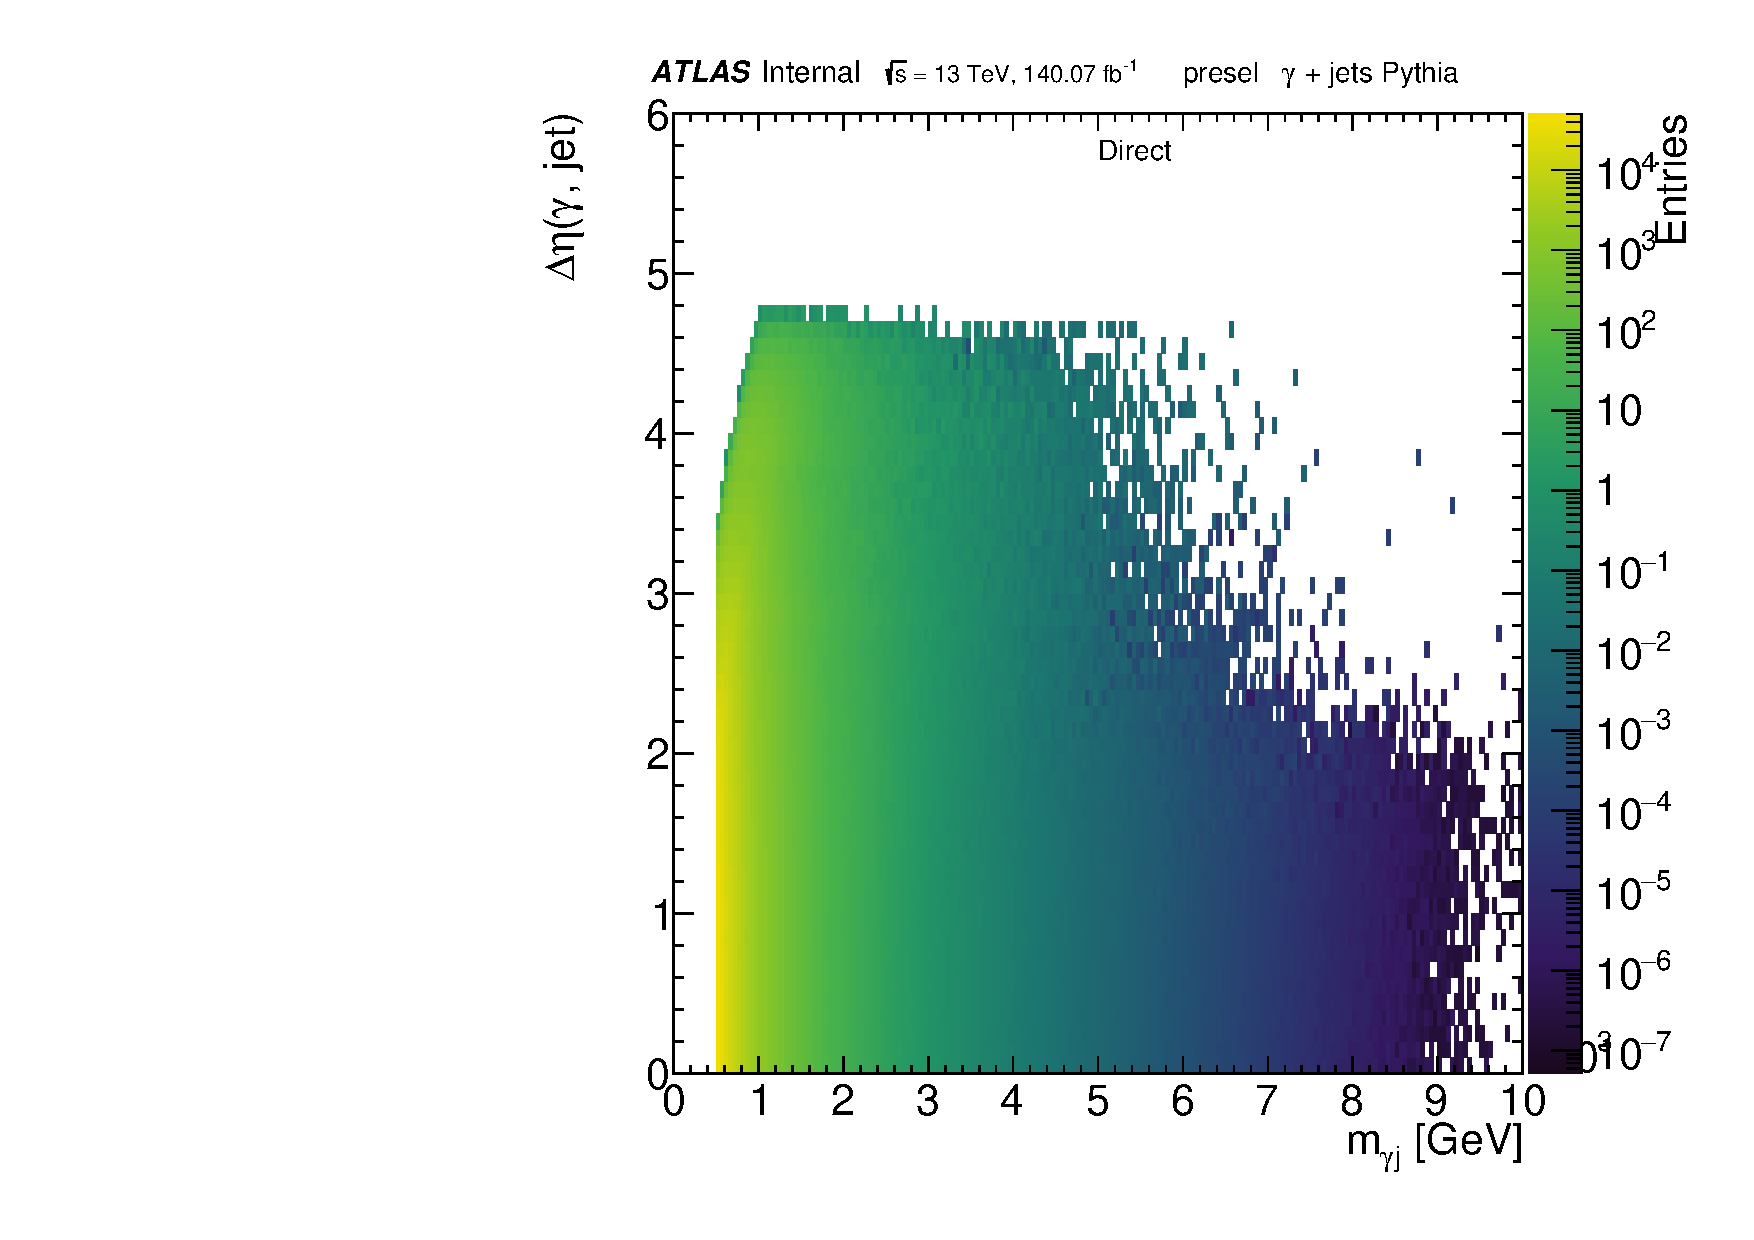
\includegraphics[width=\linewidth]{5_resonances/event_selection/deta/can2d__direct__presel__phjet_m_phjet_deta}
        \caption{Direct photons}
        \label{fig:evt_selection:sr_opt:eta:deta:2d:direct}
    \end{subfigure}
    \hfill
    \begin{subfigure}[h]{0.49\linewidth}
        \centering
        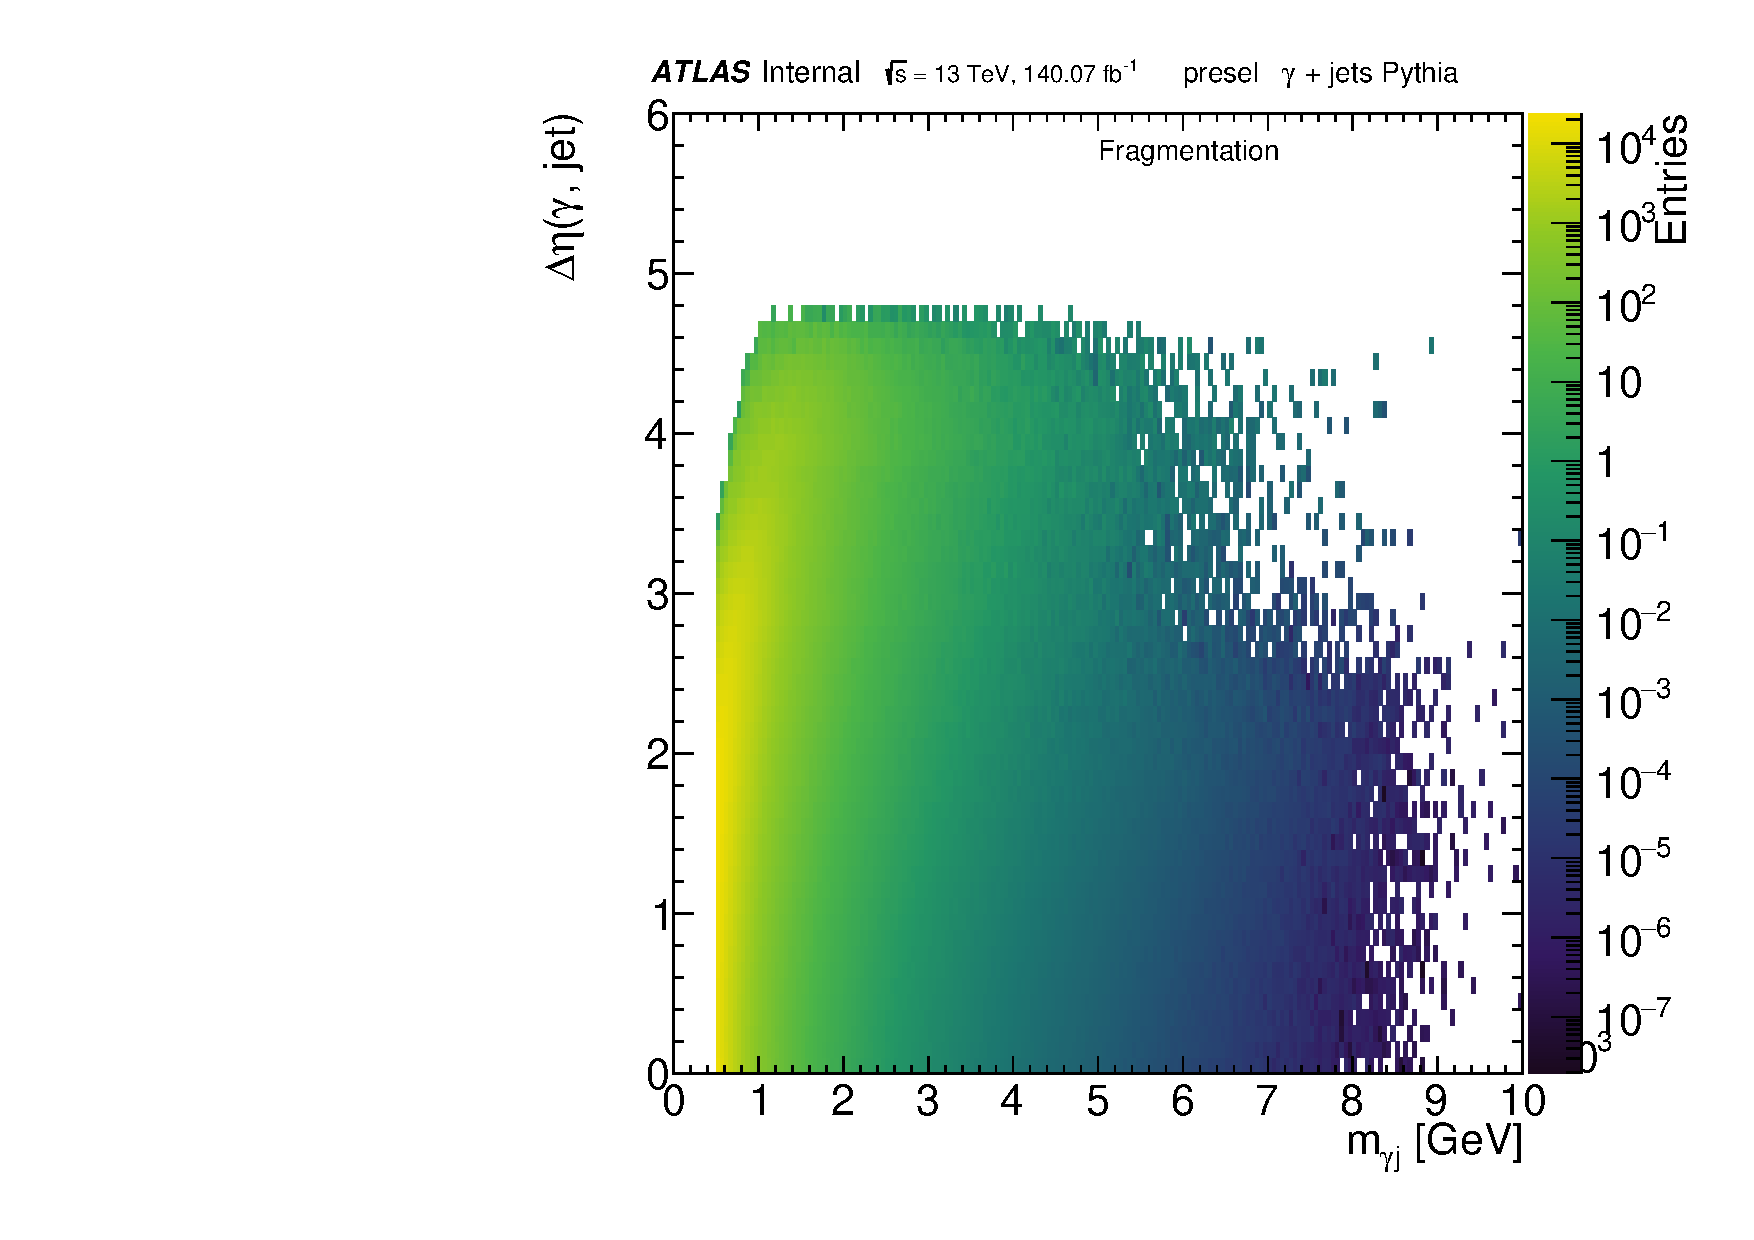
\includegraphics[width=\linewidth]{5_resonances/event_selection/deta/can2d__fragmentation__presel__phjet_m_phjet_deta}
        \caption{Fragmentation photons}
        \label{fig:evt_selection:sr_opt:eta:deta:2d:frag}
    \end{subfigure}
    \caption{\(\detayj-\myj\) 2D distribution for the \gammajet \pythia background, separating into direct (left) and fragmentation (right) photons.}
    \label{fig:evt_selection:sr_opt:eta:deta:2d}
\end{figure}


\Fig{\ref{fig:evt_selection:sr_opt:eta:deta:2d}} shows the \Deta-\myj two-dimensional distribution of the \gammajet background, separating into direct and fragmentation events.
It can be seen from these distributions there is a higher concentration of high-\detayj events for fragmentation photons compared to direct photons. This scenario es true regardless of the \myj value, but more prominent in the \(1 < \myj < 5~\tev\) region. By selecting events with low \detayj it is possible to reject a high proportion of fragmentation photons and \(t\)-channel events.

\begin{figure}[ht!]
    \centering
    \begin{subfigure}[h]{0.49\linewidth}
        \centering
        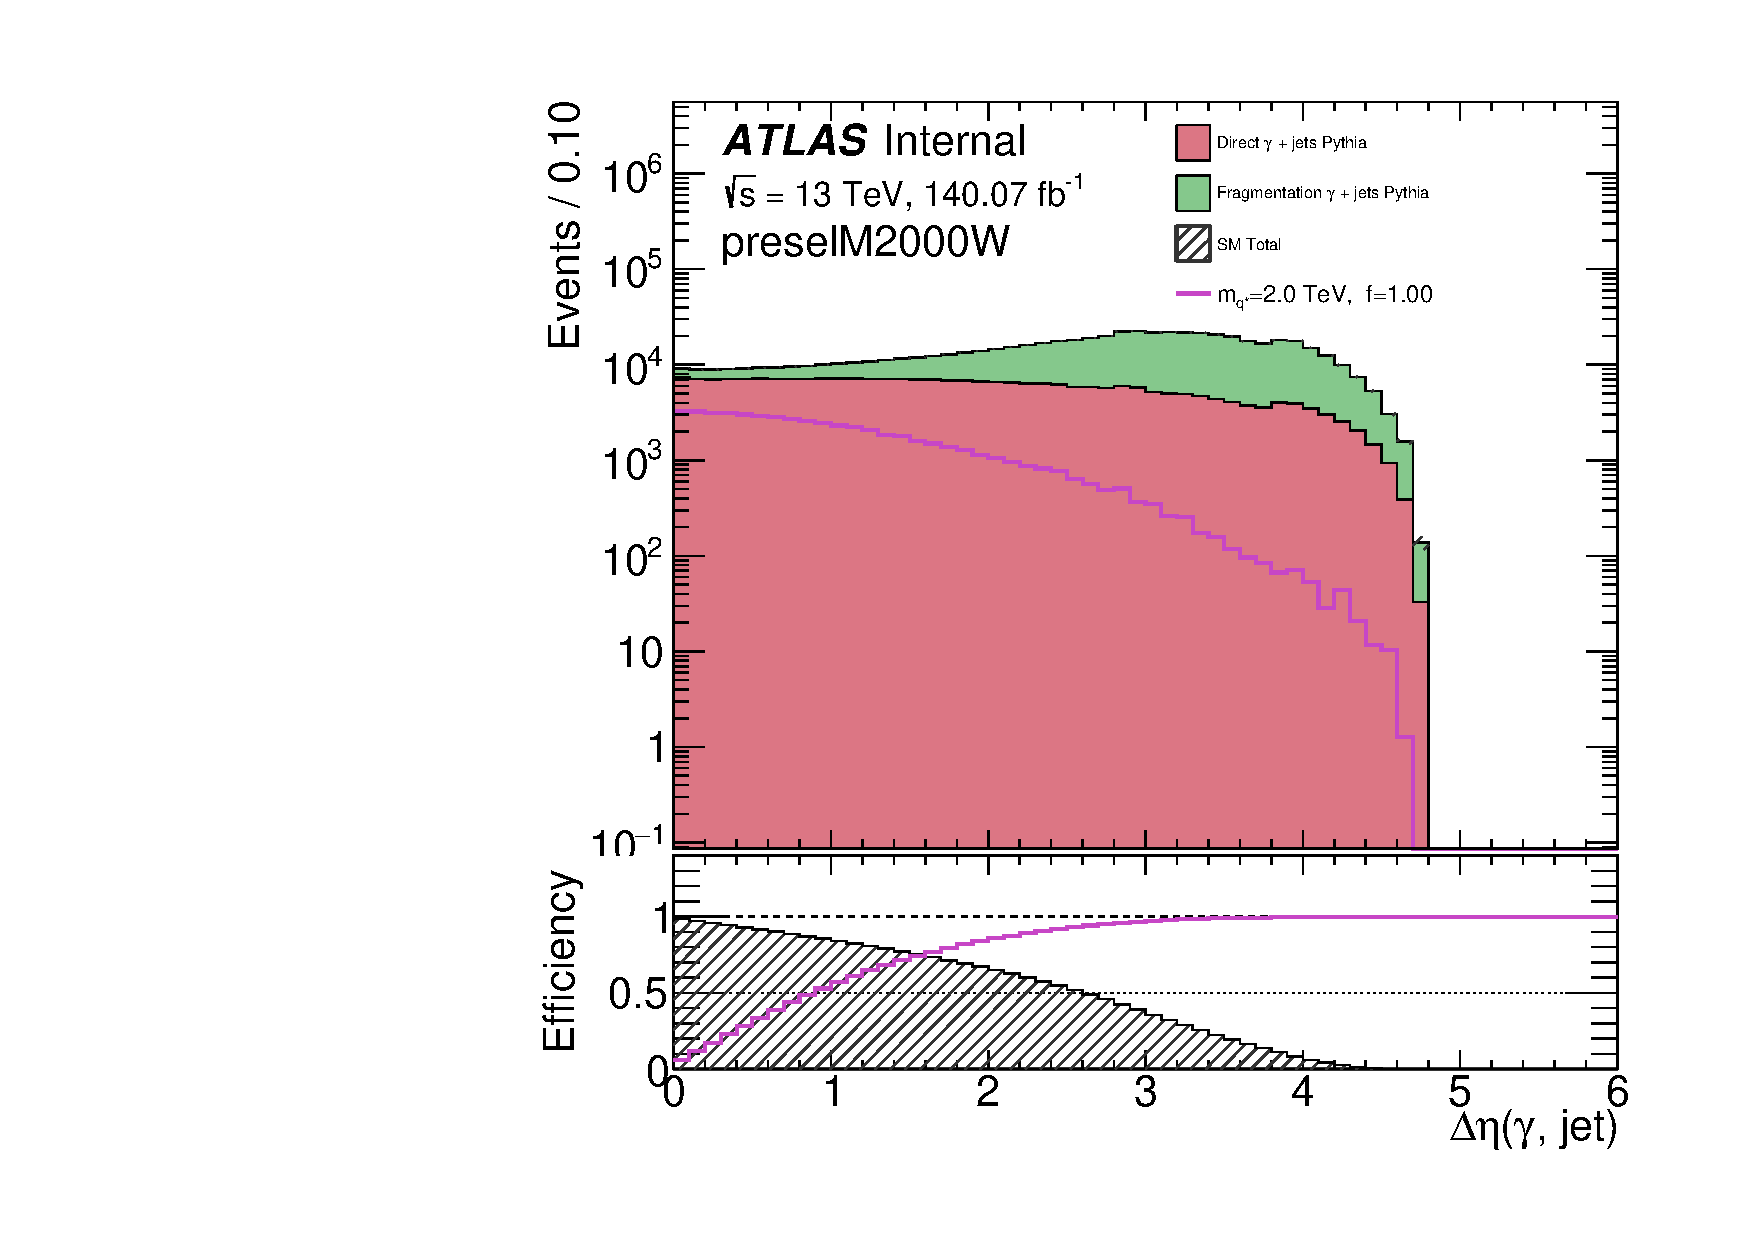
\includegraphics[width=\textwidth]{5_resonances/event_selection/deta/1d/preselM2000W/bkg_sig/1d/no_normalized/can__photonjet_Pythia_sig__preselM2000W__phjet_deta__wsignals_models__qStar_M2000__Run2__effrej}
        \caption{\(1000~\gev < \myj < 3000~\gev\)}
        \label{fig:evt_selection:sr_opt:eta:deta:1d:effrej_2000W}
    \end{subfigure}
    \hfill
    \begin{subfigure}[h]{0.49\linewidth}
        \centering
        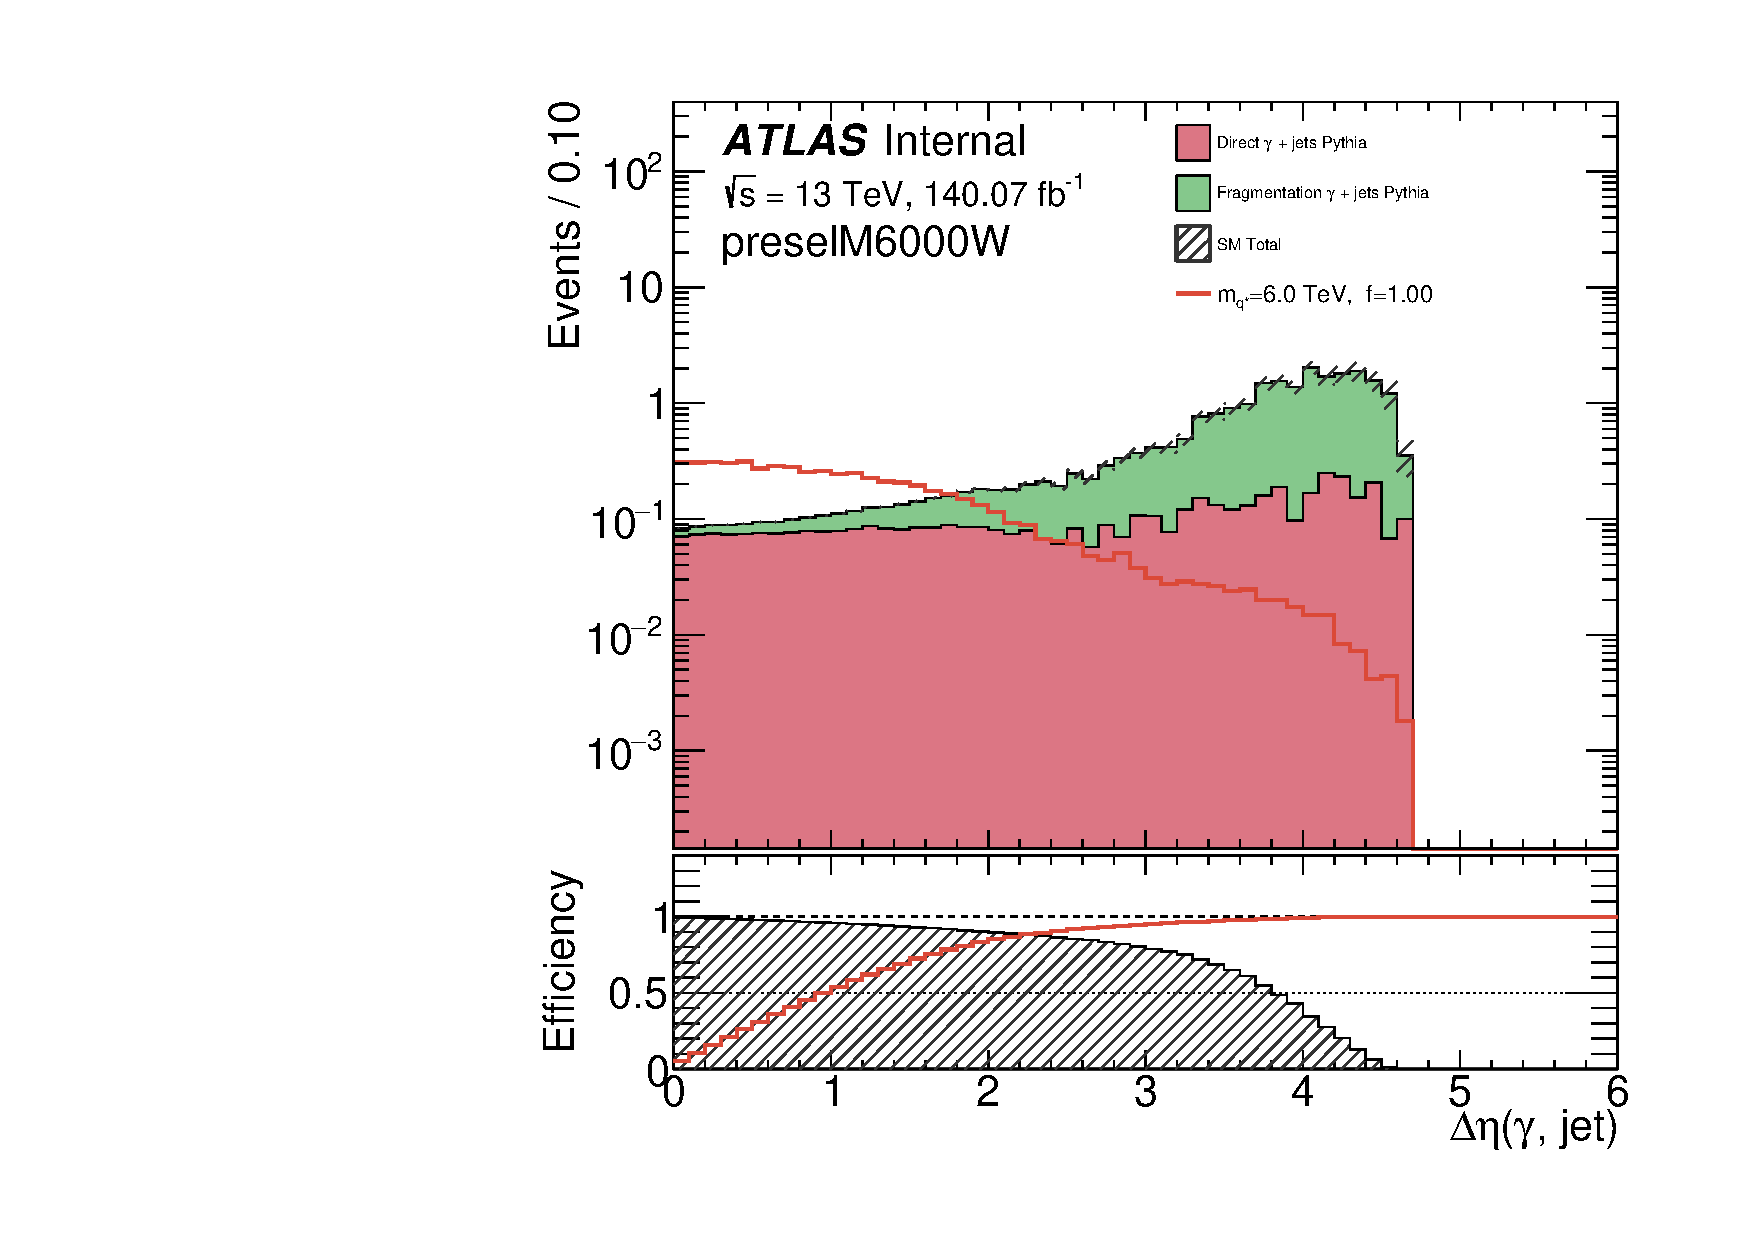
\includegraphics[width=\textwidth]{5_resonances/event_selection/deta/1d/preselM6000W/bkg_sig/1d/no_normalized/can__photonjet_Pythia_sig__preselM6000W__phjet_deta__wsignals_models__qStar_M6000__Run2__effrej}
        \caption{\(5000~\gev < \myj < 7000~\gev\)}
        \label{fig:evt_selection:sr_opt:eta:deta:1d:effrej_6000W}
    \end{subfigure}\\
    \begin{subfigure}[h]{0.49\linewidth}
        \centering
        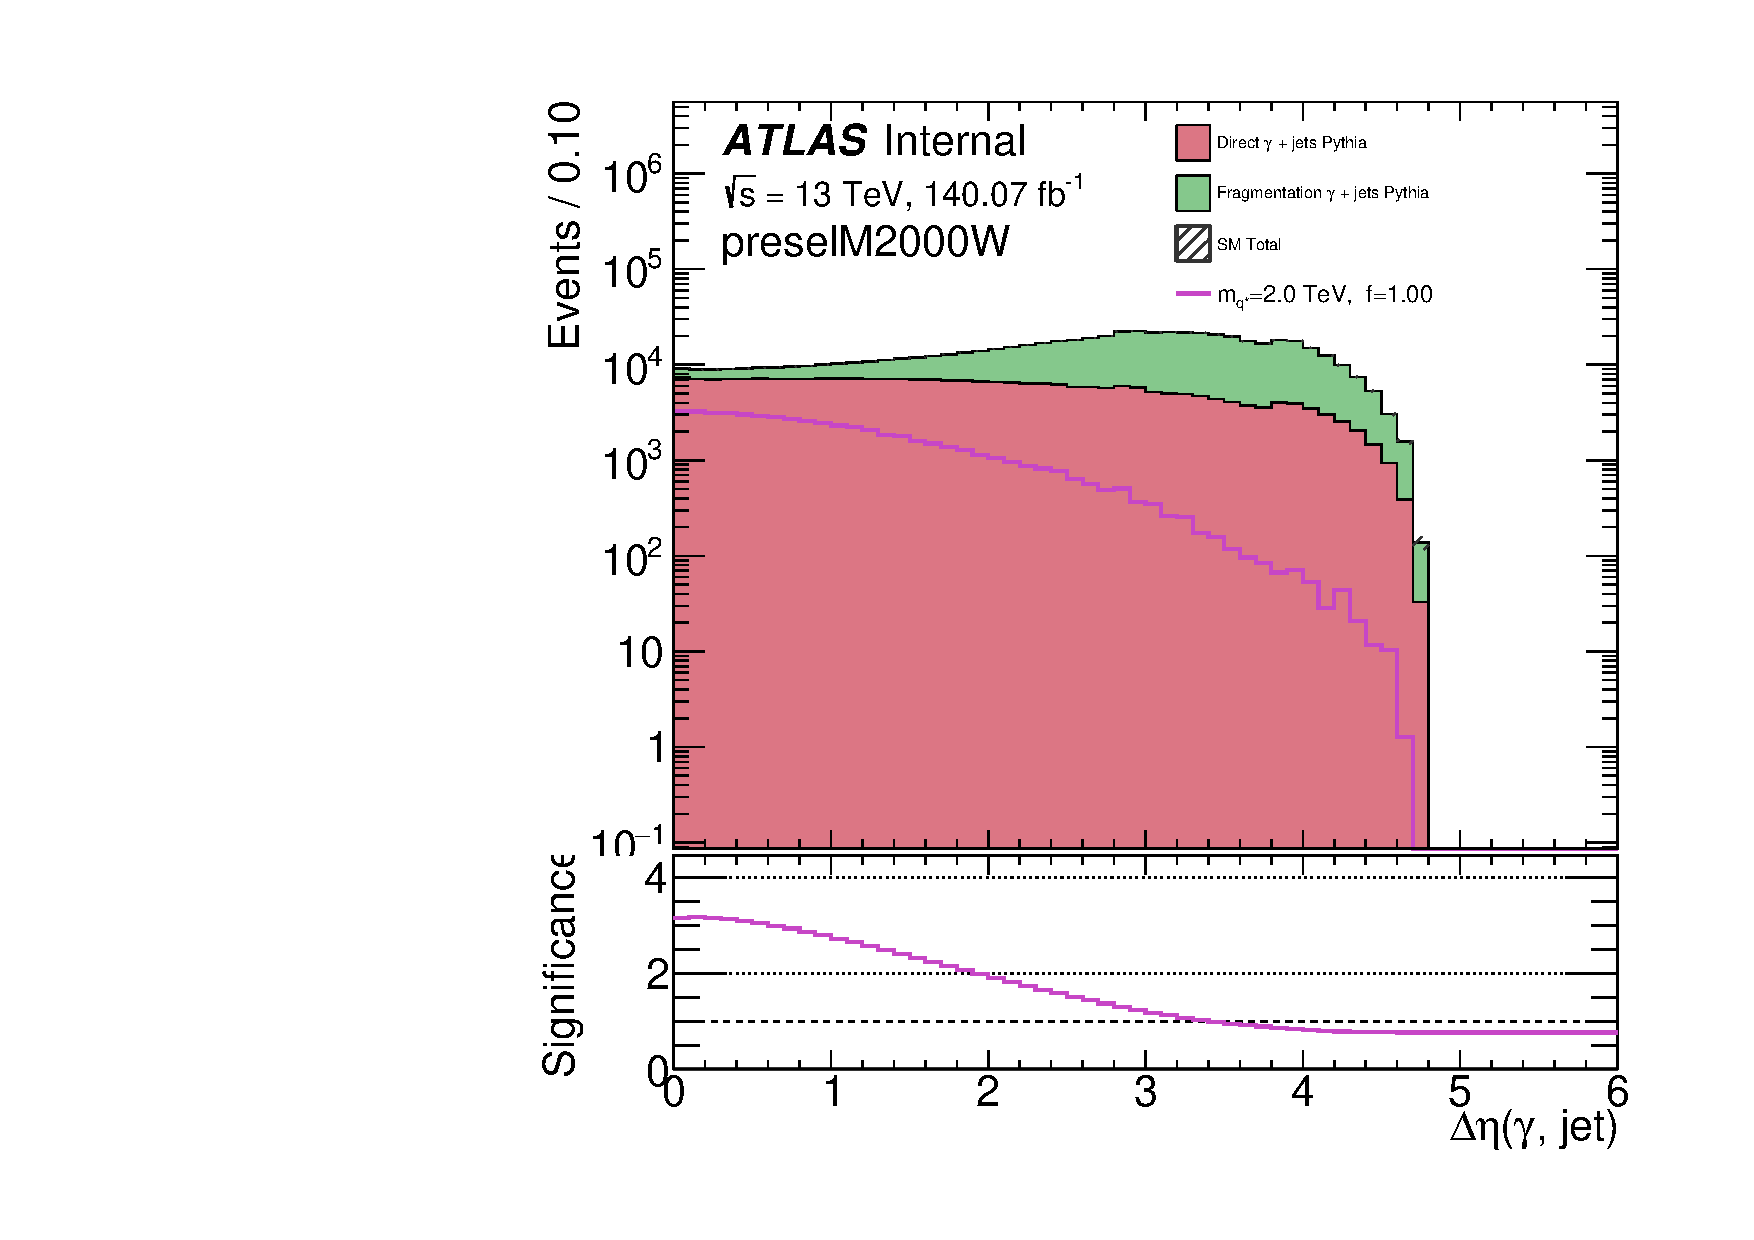
\includegraphics[width=\textwidth]{5_resonances/event_selection/deta/1d/preselM2000W/bkg_sig/1d/no_normalized/can__photonjet_Pythia_sig__preselM2000W__phjet_deta__wsignals_models__qStar_M2000__Run2__SB_significance}
        \caption{\(1000~\gev < \myj < 3000~\gev\)}
        \label{fig:evt_selection:sr_opt:eta:deta:1d:SB_2000W}
    \end{subfigure}
    \hfill
    \begin{subfigure}[h]{0.49\linewidth}
        \centering
        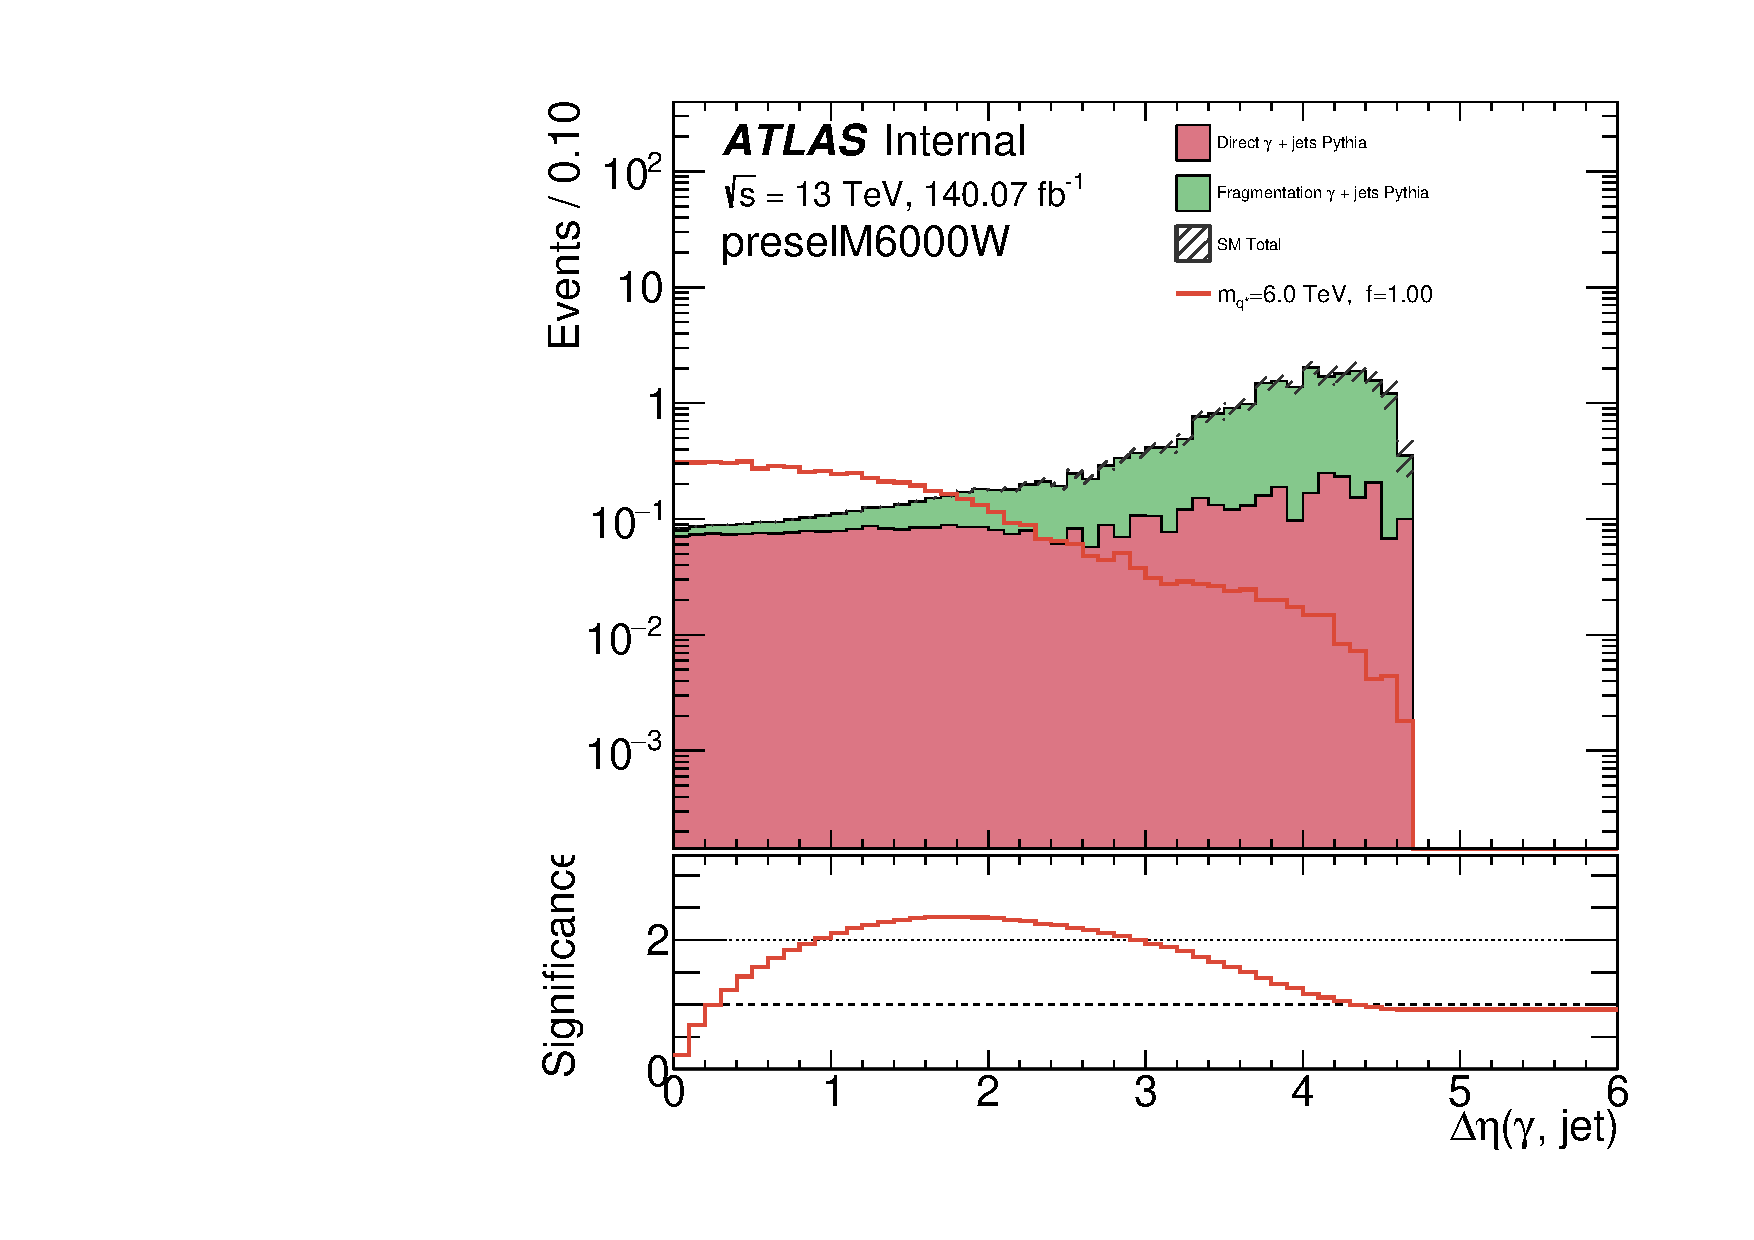
\includegraphics[width=\textwidth]{5_resonances/event_selection/deta/1d/preselM6000W/bkg_sig/1d/no_normalized/can__photonjet_Pythia_sig__preselM6000W__phjet_deta__wsignals_models__qStar_M6000__Run2__SB_significance}
        \caption{\(5000~\gev < \myj < 7000~\gev\)}
        \label{fig:evt_selection:sr_opt:eta:deta:1d:SB_6000W}
    \end{subfigure}
    \caption{\(\deta{\gamma}{j}\) distribution in two \myj windows comparison between background and signal models. The bottom pads in \Figs{\ref{fig:evt_selection:sr_opt:eta:deta:1d:effrej_2000W}}{\ref{fig:evt_selection:sr_opt:eta:deta:1d:effrej_6000W}} show the signals efficiencies (coloured lines) and background rejection (hashed histogram) if a cut of the type \(\Deta < X\) is applied. On the contrary, on \Figs{\ref{fig:evt_selection:sr_opt:eta:deta:1d:SB_2000W}}{\ref{fig:evt_selection:sr_opt:eta:deta:1d:SB_6000W}}, the bottom pad shows the signal significance. The \yj events were modelled with \pythia.}
    \label{fig:evt_selection:sr_opt:eta:deta:1d}
\end{figure}

Comparisons of background with signal models using this variable are shown in \Fig{\ref{fig:evt_selection:sr_opt:eta:deta:1d}}. The selection in these figures corresponds on selecting events with \(\mq - 1000 < \myj < \mq + 1000 ~\gev\), which consists on a \(2~\tev\) mass window around the signal model's mass.
The bottom pad in \Figs{\ref{fig:evt_selection:sr_opt:eta:deta:1d:effrej_2000W}}{\ref{fig:evt_selection:sr_opt:eta:deta:1d:effrej_6000W}} show the efficiency on the signals for the coloured lines, while the hashed histogram shows the background rejection if a cut of the type \(\Deta < X\) is applied. From these, it can be seen that a cut to this variable at \(\Deta \approx 1.6\) would help reduce background considerabely (\(\sim 80\%\)) while keeping most of the signal events (efficiency \(60-80\%\)).
Further studies have been carried out as well computing the significance of this cut. \Figs{\ref{fig:evt_selection:sr_opt:eta:deta:1d:SB_2000W}}{\ref{fig:evt_selection:sr_opt:eta:deta:1d:SB_6000W}}, show in the bottom pads the signal significance for the same cases.
Excepting the trivial cut on \(\Deta = 0\), it can be noted that for higher \myj values maximum significance can be achieved by selecting events with \(\deta{\gamma}{j} \lesssim 1.6\), and for this reason, it has been opted to apply the cut \(\deta{\gamma}{j} < 1.6\) for the rest of the analysis.
Another important aspect that can be seen from these figures is the fact thath the majority of fragmentation photon events \enquote{live} in the high-\Deta region, as anticipated from \Fig{\ref{fig:evt_selection:sr_opt:eta:deta:2d:frag}}. By applying this cut, fragmentation photon events are highly reduced.


\subsubsection{Photon and jet pseudorapidity}
\label{subsubsec:evt_selection:sr_opt:eta:etas}

In the low mass region \(\myj \lesssim 3~\tev\), there is a high background concentration of events with \(\etagam > 1.37\) and \(\etajet > 1.37\), compared to the benchmark signals, as seen from \Fig{\ref{fig:evt_selection:sr_opt:eta:etas:1d}}. For this reason, by applying a cut on these two variables the signal-to-background ratio would increase with almost no cost on the signal significance nor efficiency, as shown in the bottom pads of the figures. Therefore, it is decided that events with \(\etagam > 1.37\) and \(\etajet > 1.37\) are removed.

\begin{figure}[ht!]
    \centering
    \begin{subfigure}[h]{0.49\linewidth}
        \centering
        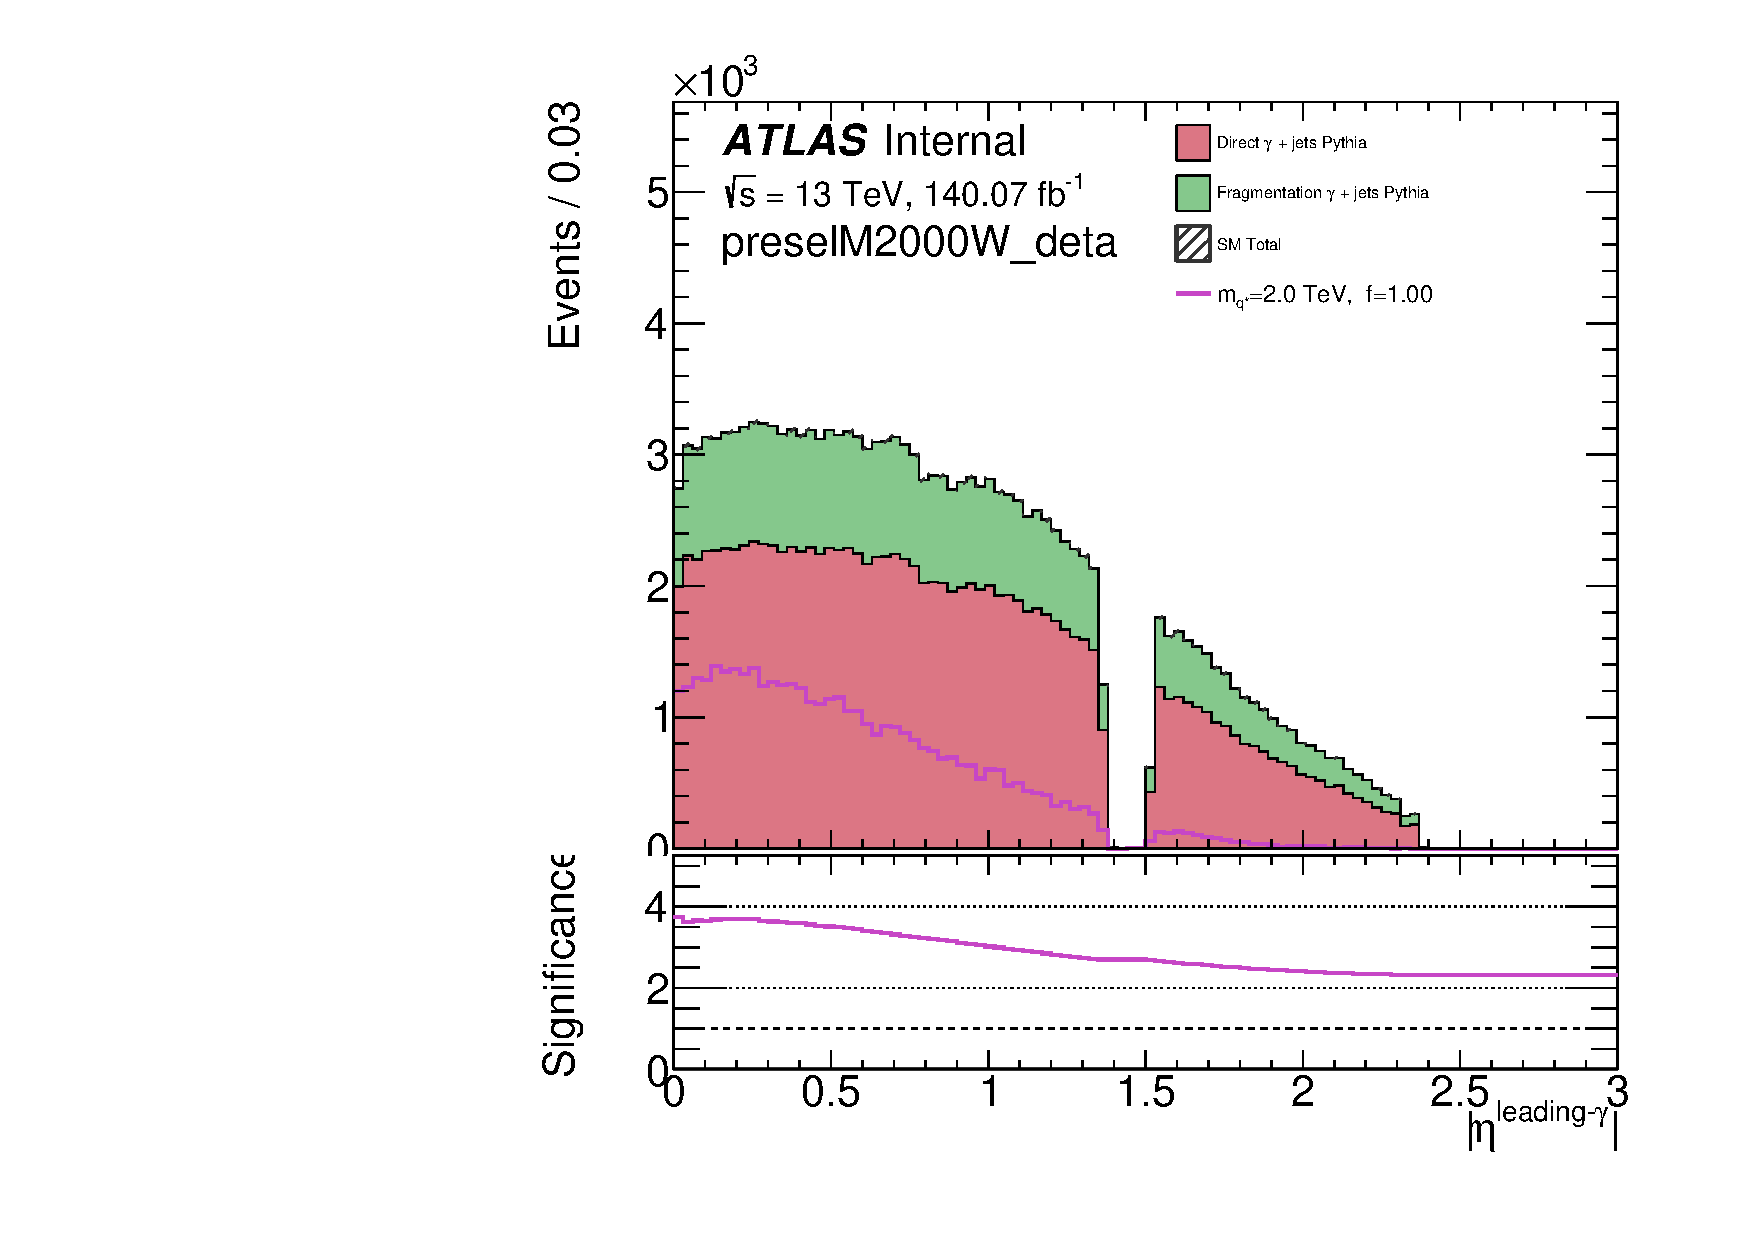
\includegraphics[width=\textwidth]{5_resonances/event_selection/eta/preselM2000W_deta/bkg_sig/1d/no_normalized/can__photonjet_Pythia_sig__preselM2000W_deta__absph_eta0__wsignals_models__qStar_M2000__Run2__SB_significance}
        \caption{\etagam}
        \label{fig:evt_selection:sr_opt:eta:etas:1d:ph}
    \end{subfigure}
    \hfill
    \begin{subfigure}[h]{0.49\linewidth}
        \centering
        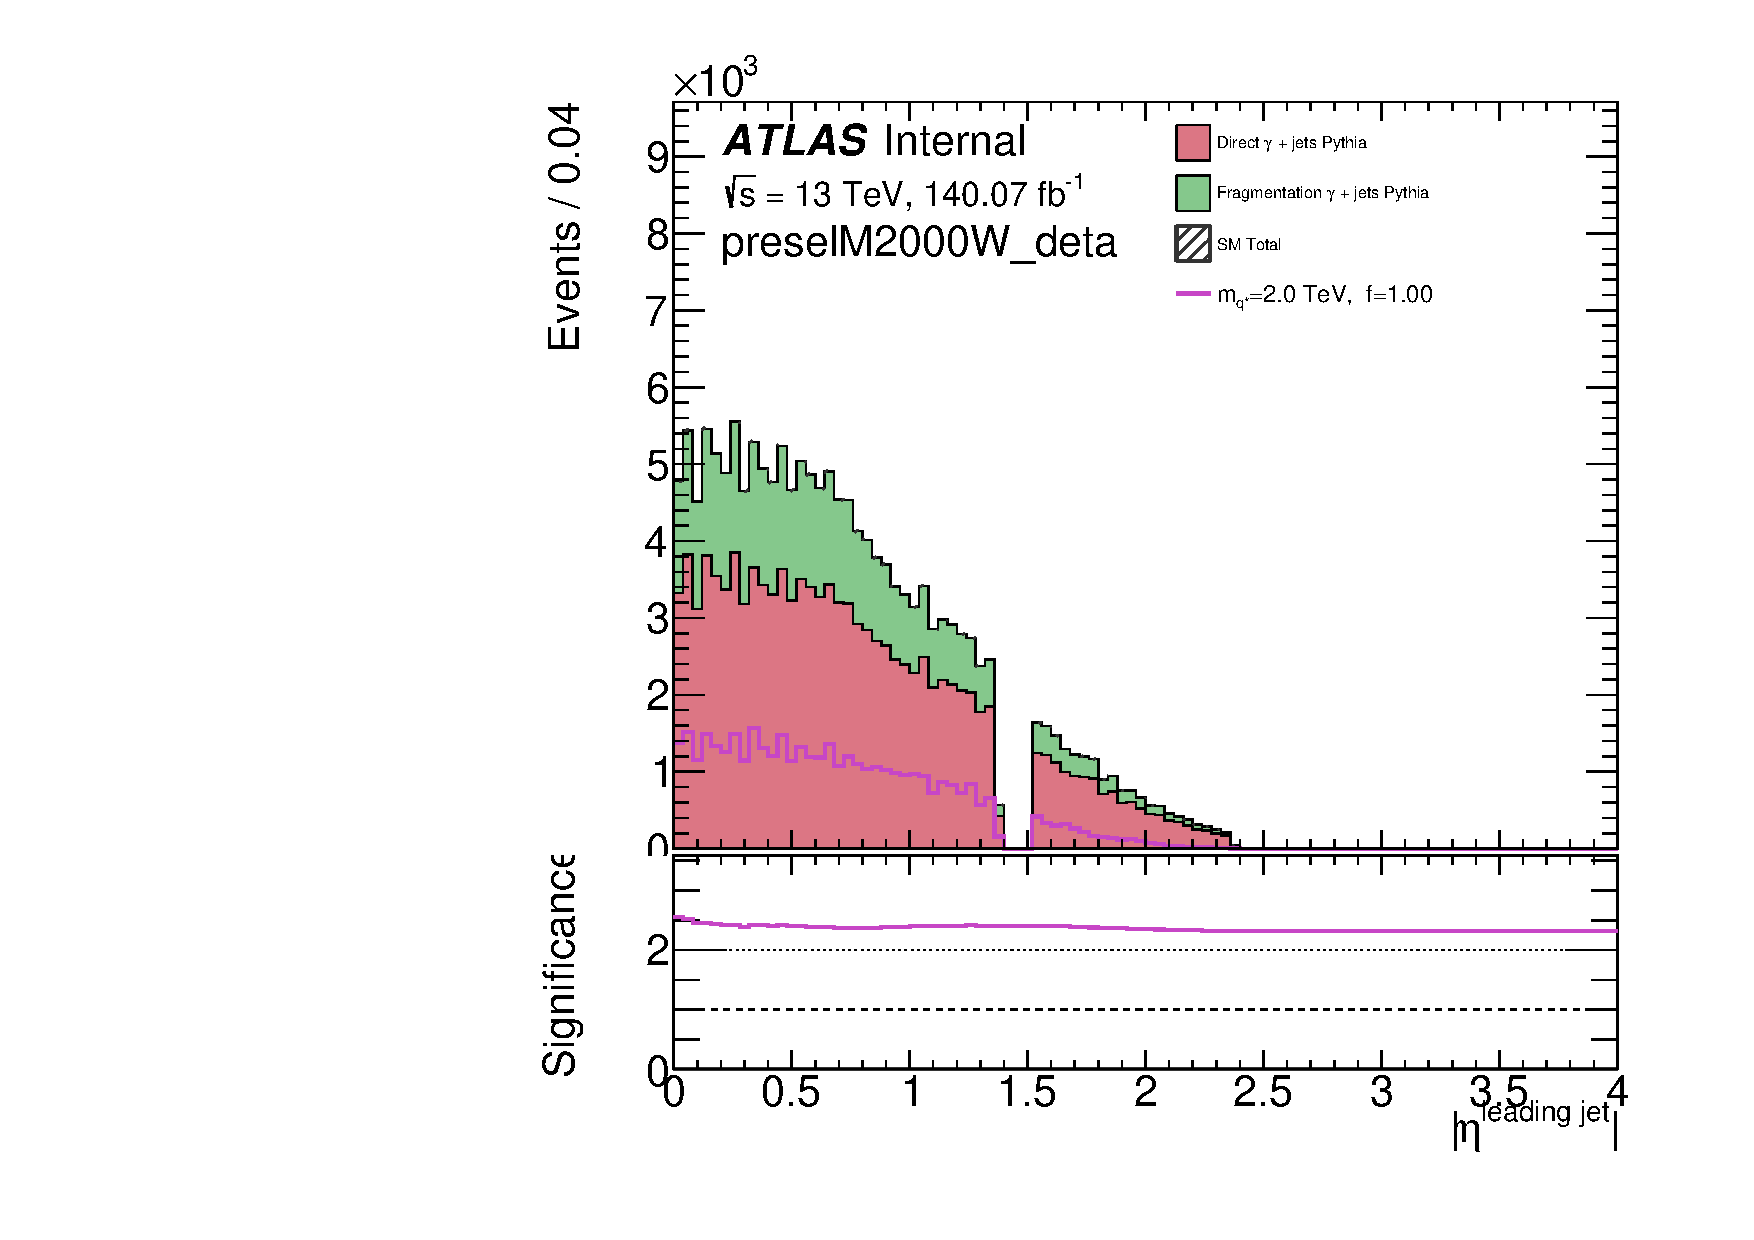
\includegraphics[width=\textwidth]{5_resonances/event_selection/eta/preselM2000W_deta/bkg_sig/1d/no_normalized/can__photonjet_Pythia_sig__preselM2000W_deta__absjet_eta0__wsignals_models__qStar_M2000__Run2__SB_significance}
        \caption{\etajet}
        \label{fig:evt_selection:sr_opt:eta:etas:1d:jet}
    \end{subfigure}
    \caption{\etagam and \etajet distributions in a window of \(1000~\gev < \myj < 3000~\gev\) comparing signals with the main \yj \pythia background. Bottom pads show signals significances over the background.}
    \label{fig:evt_selection:sr_opt:eta:etas:1d}
\end{figure}



\subsection{Extended isolation}
\label{subsec:evt_selection:sr_opt:extended_iso}

The photon reconstruction, identification and isolation cuts on photons act to reduce instrumental backgrounds (misidentified hadrons) to a negligible level, but some of the substantial background from secondary (fragmentation) photons remains.
To further reduce this background, the contribution to the leading photon isolation energy from jets close to it is investigated, after applying all the selections shown above.

\begin{figure}[ht!]
    \centering
    \begin{subfigure}[t]{0.49\linewidth}
        \centering
        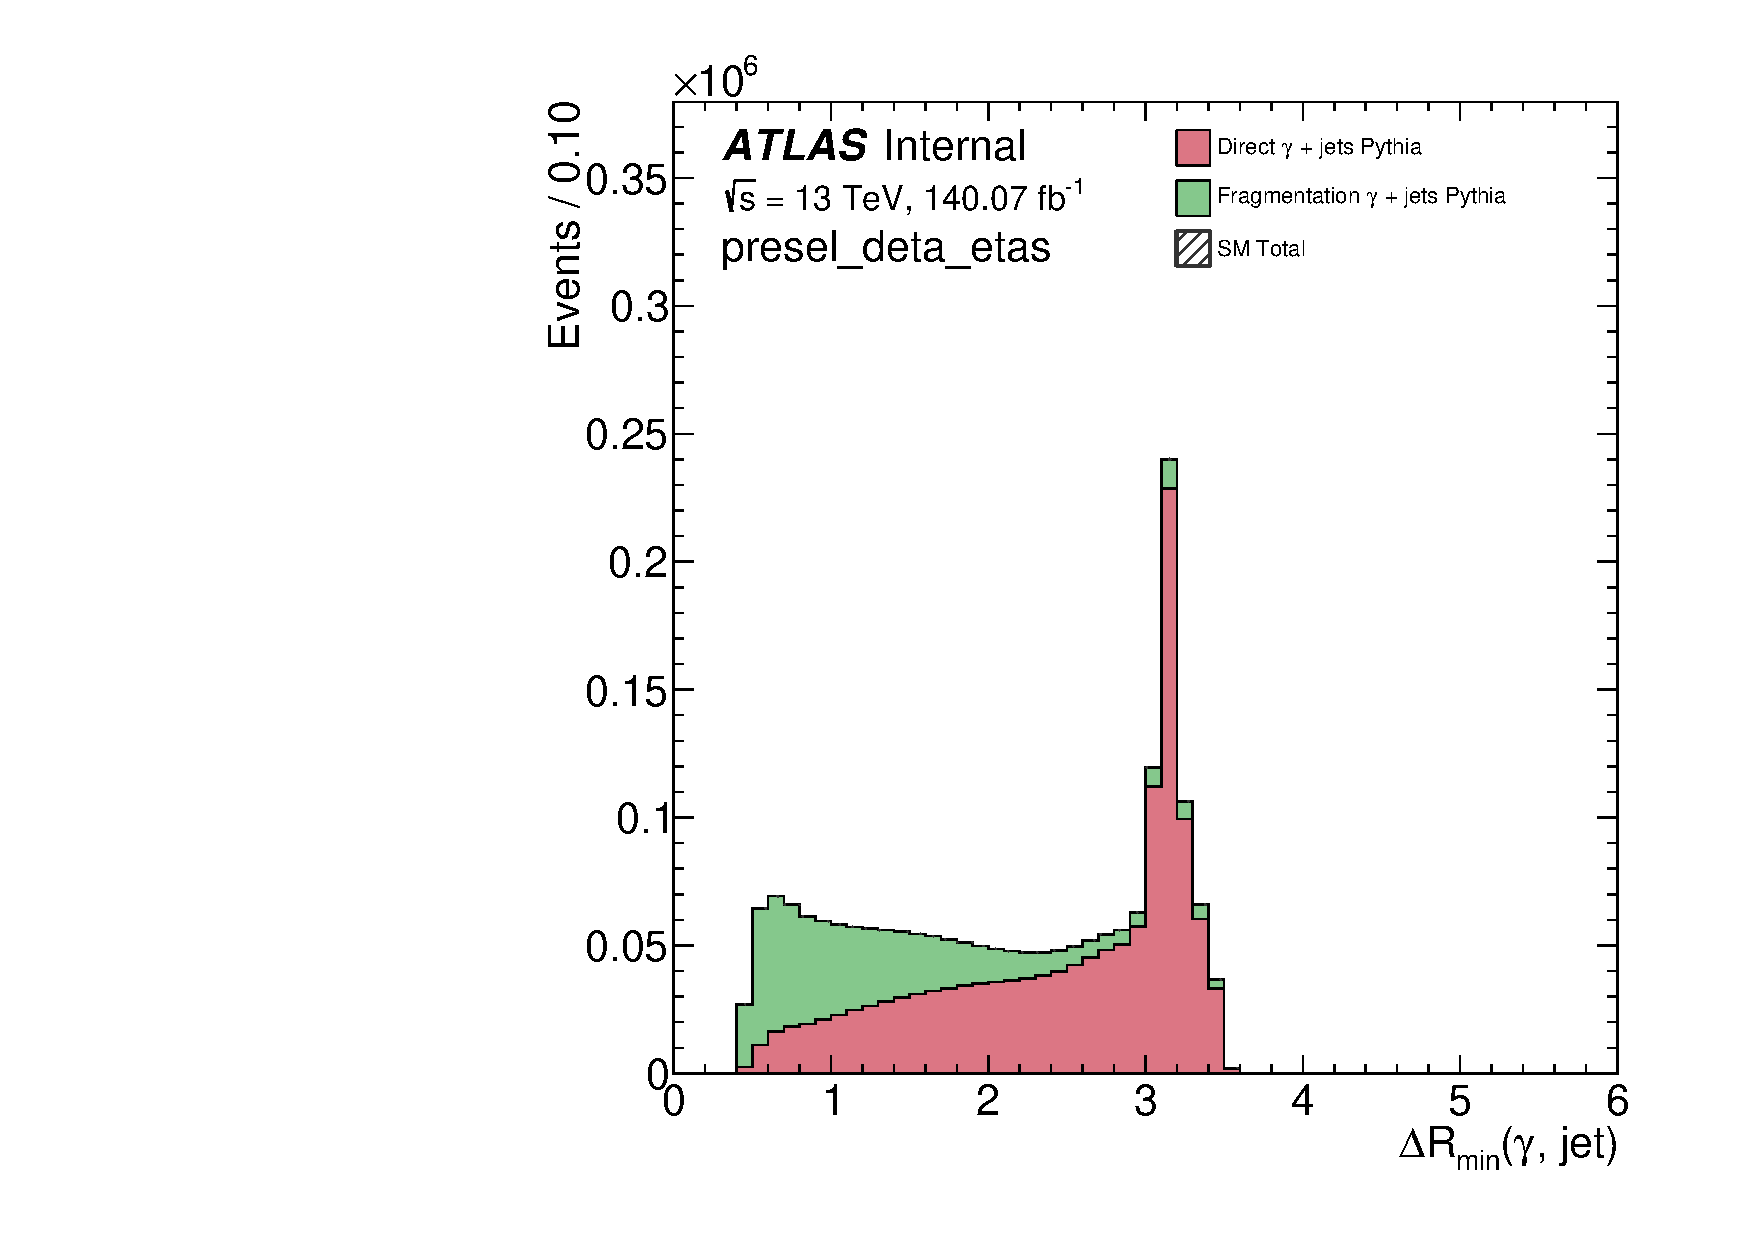
\includegraphics[width=\linewidth]{5_resonances/event_selection/extended_iso/can__photonjet_Pythia__presel_deta_etas__phjet_drmin__Run2}
        \caption{Separation into direct and fragmentation photon events.}
        \label{fig:evt_selection:sr_opt:extended_iso:phjet_drmin:frag_direct}
    \end{subfigure}
    \hfill
    \begin{subfigure}[t]{0.49\linewidth}
        \centering
        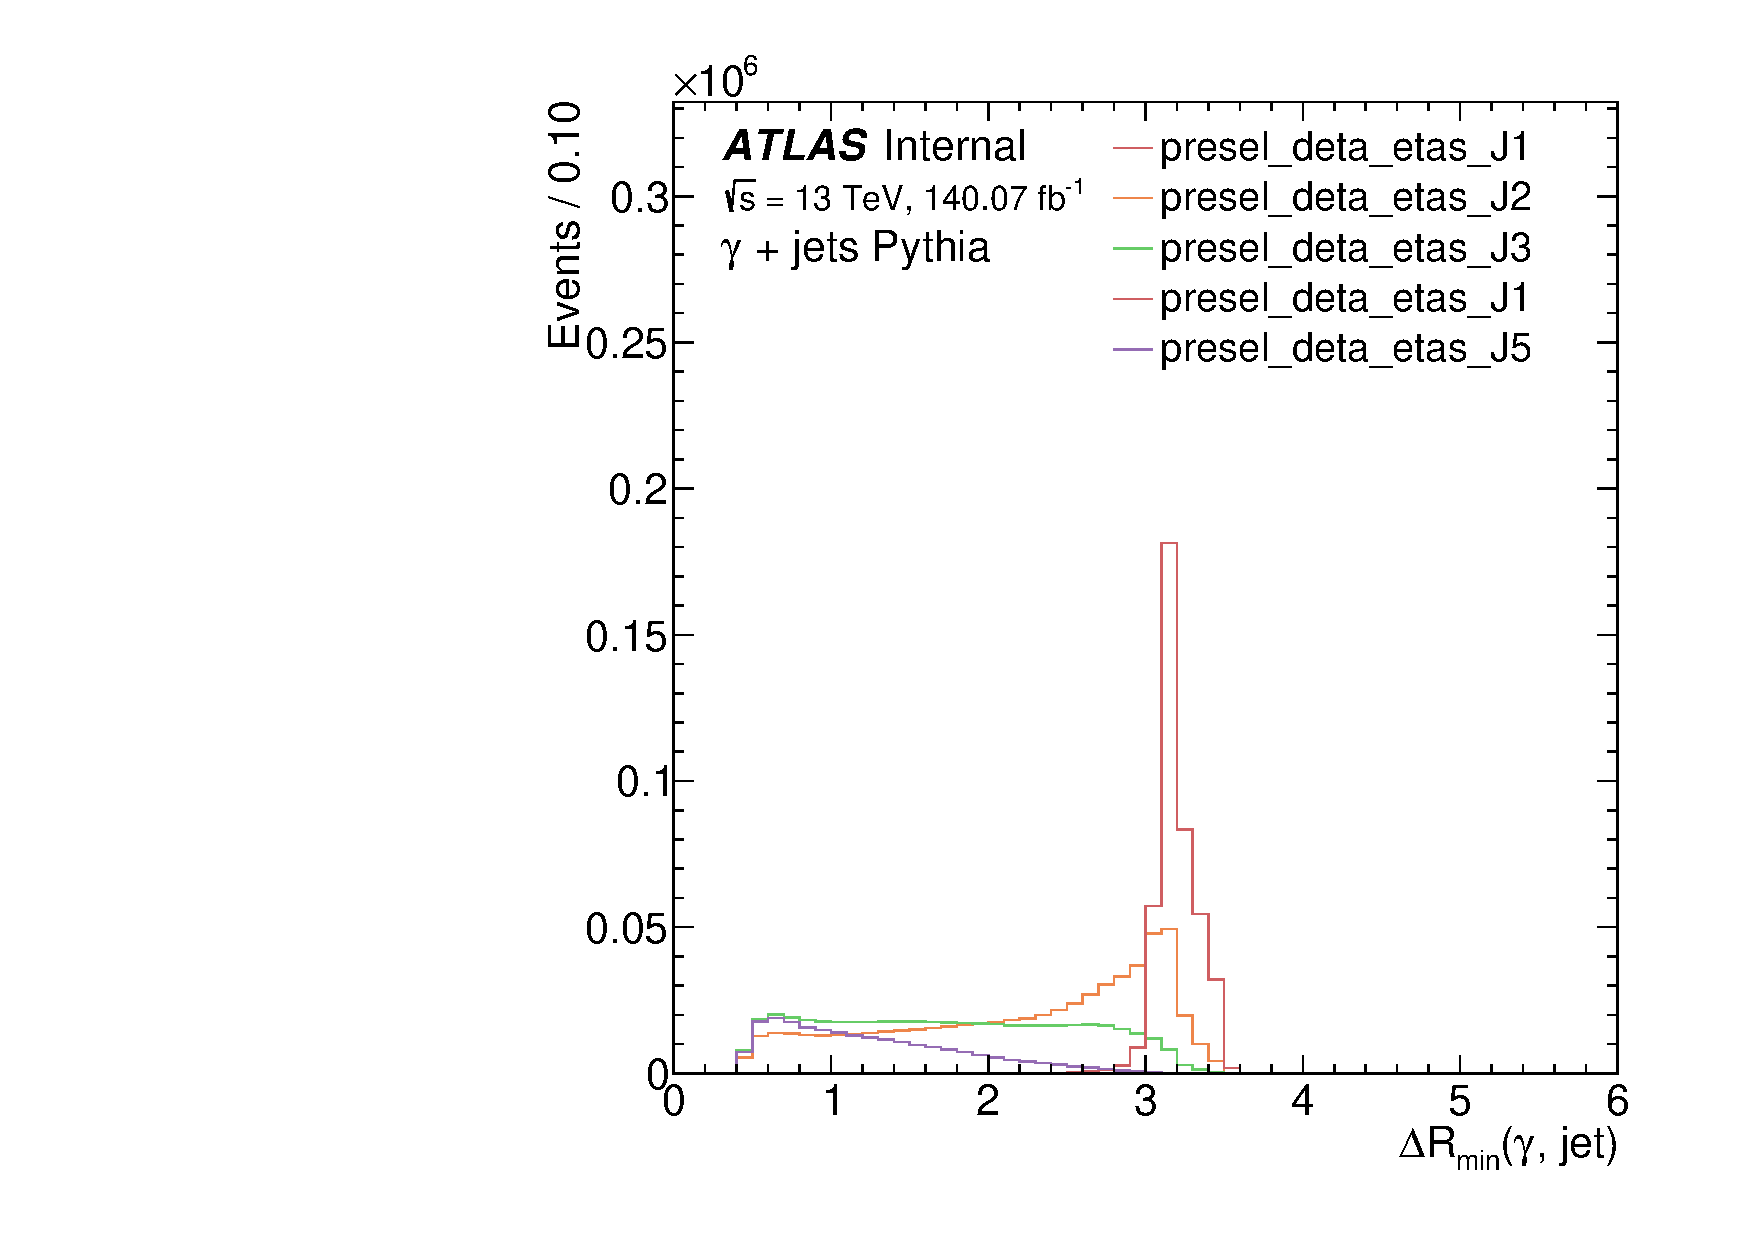
\includegraphics[width=\linewidth]{5_resonances/event_selection/extended_iso/can__photonjet_Pythia__phjet_drmin__regions_presel_deta_etas_J1_presel_deta_etas_J2_presel_deta_etas_J3_presel_deta_etas_J1_presel_deta_etas_J5__Run2}
        \caption{Separation into jet multiplicity.}
        \label{fig:evt_selection:sr_opt:extended_iso:phjet_drmin:njets}
    \end{subfigure}
    
    \caption{\(\DeltaR_{\text{min}}\) distribution for the \gammajet \pythia background. This variable shows the minimum distance found between the leading photon and any of the jets.}
    \label{fig:evt_selection:sr_opt:extended_iso:phjet_drmin}
\end{figure}

In \Fig{\ref{fig:evt_selection:sr_opt:extended_iso:phjet_drmin:frag_direct}}, the distribution of \(\DeltaR_{\text{min}}\) is shown, separating between fragmentation and direct photon events. Said variable, measures the angular distance between the leading photon and the closest jet to the photon. From this distribution it is possible to note that the majority of events very close to the photon (small \(\DeltaR_{\text{min}}\)) are fragmentation events.
Furthermore, the contribution to the said distribution can be seen for events which have different jet multiplicity (\njet), shown in \Fig{\ref{fig:evt_selection:sr_opt:extended_iso:phjet_drmin:njets}}. It is known that fragmentation photon events contain more jets than those events coming from direct photon production, and with higher jet multiplicity, the higher the probabilities are that a jet is very close to the photon, contributing to the isolation energy of it.


\begin{figure}[ht!]
    \centering
    \begin{subfigure}[t]{0.49\linewidth}
        \centering
        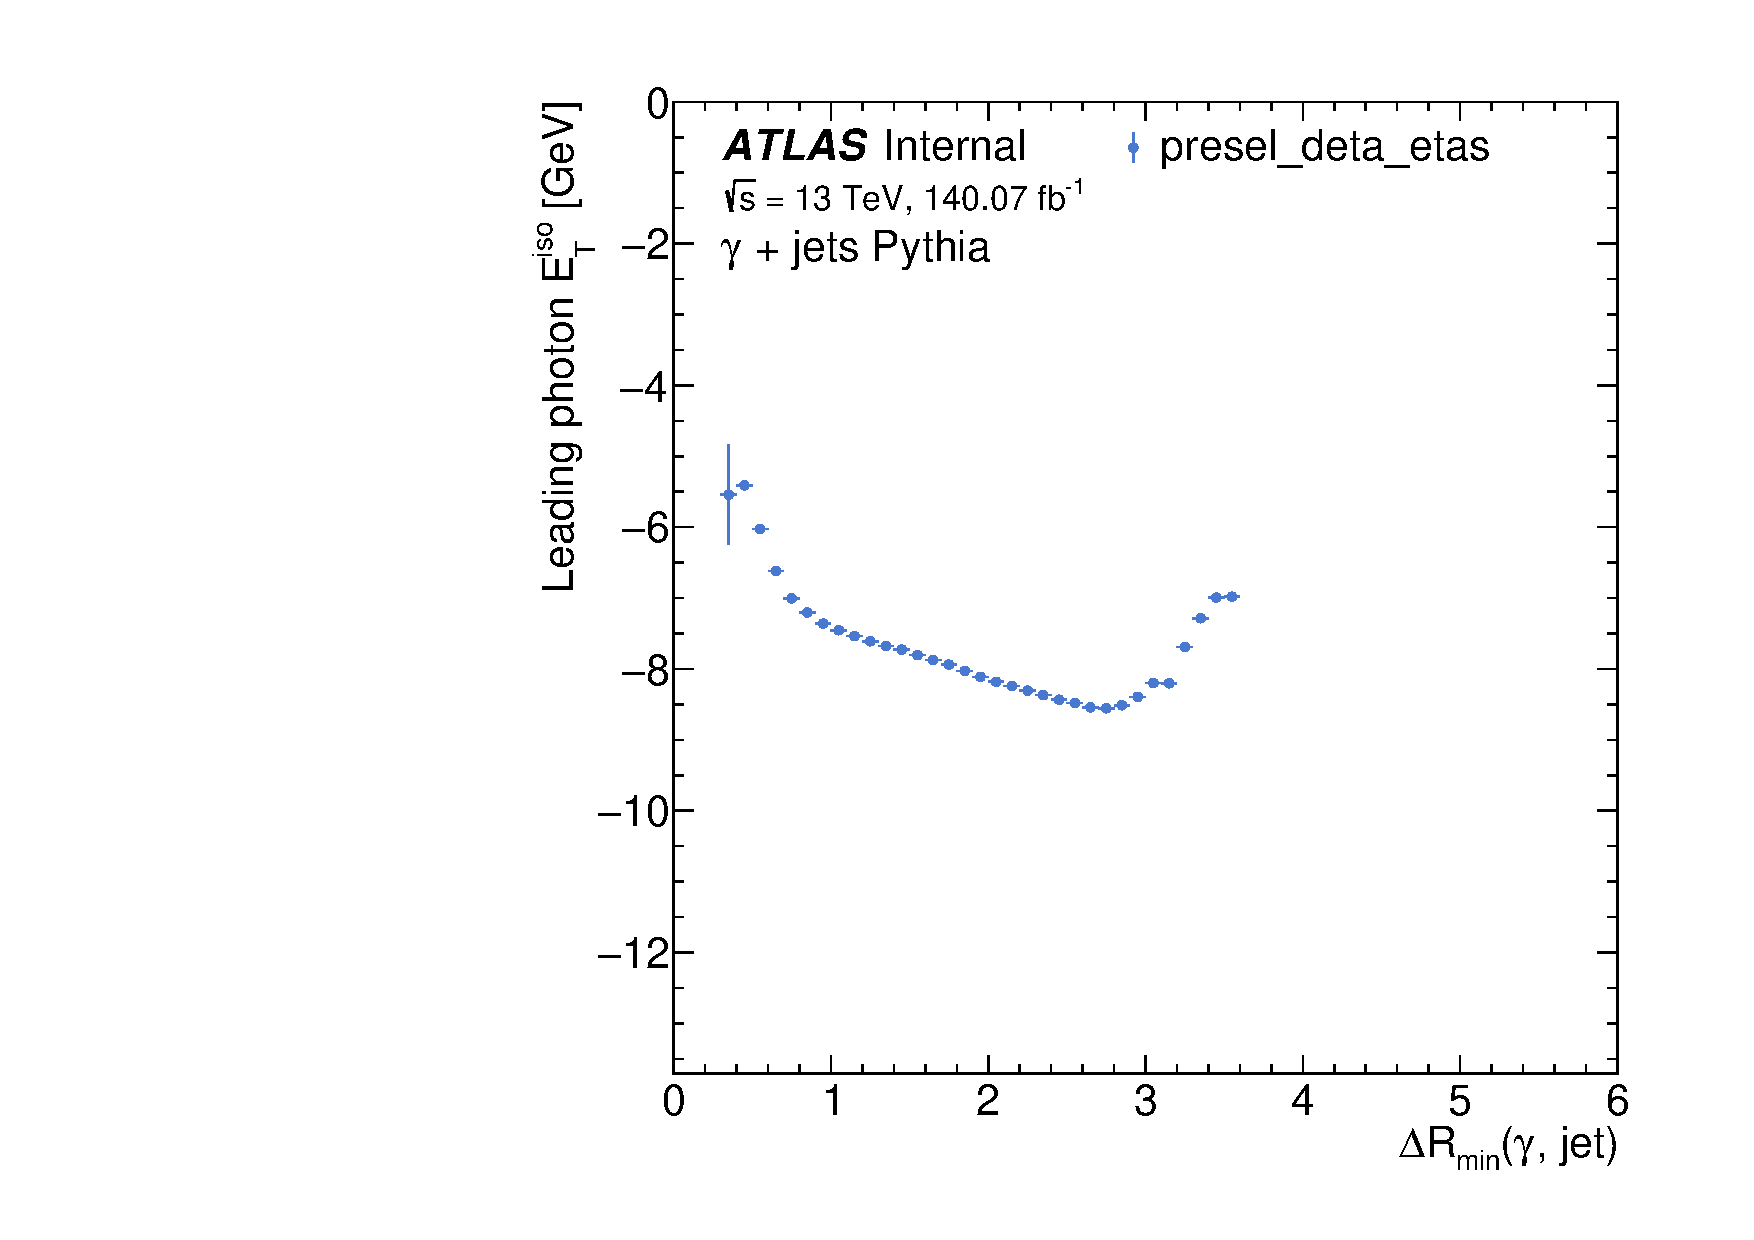
\includegraphics[width=\linewidth]{5_resonances/event_selection/extended_iso/can__photonjet_Pythia__phjet_drmin_ph_caloiso0__regions_presel_deta_etas__Run2}
        \caption{Full direct+fragmentation contribution.}
        \label{fig:evt_selection:sr_opt:extended_iso:phjet_drmin:etiso:full}
    \end{subfigure}
    \hfill
    \begin{subfigure}[t]{0.49\linewidth}
        \centering
        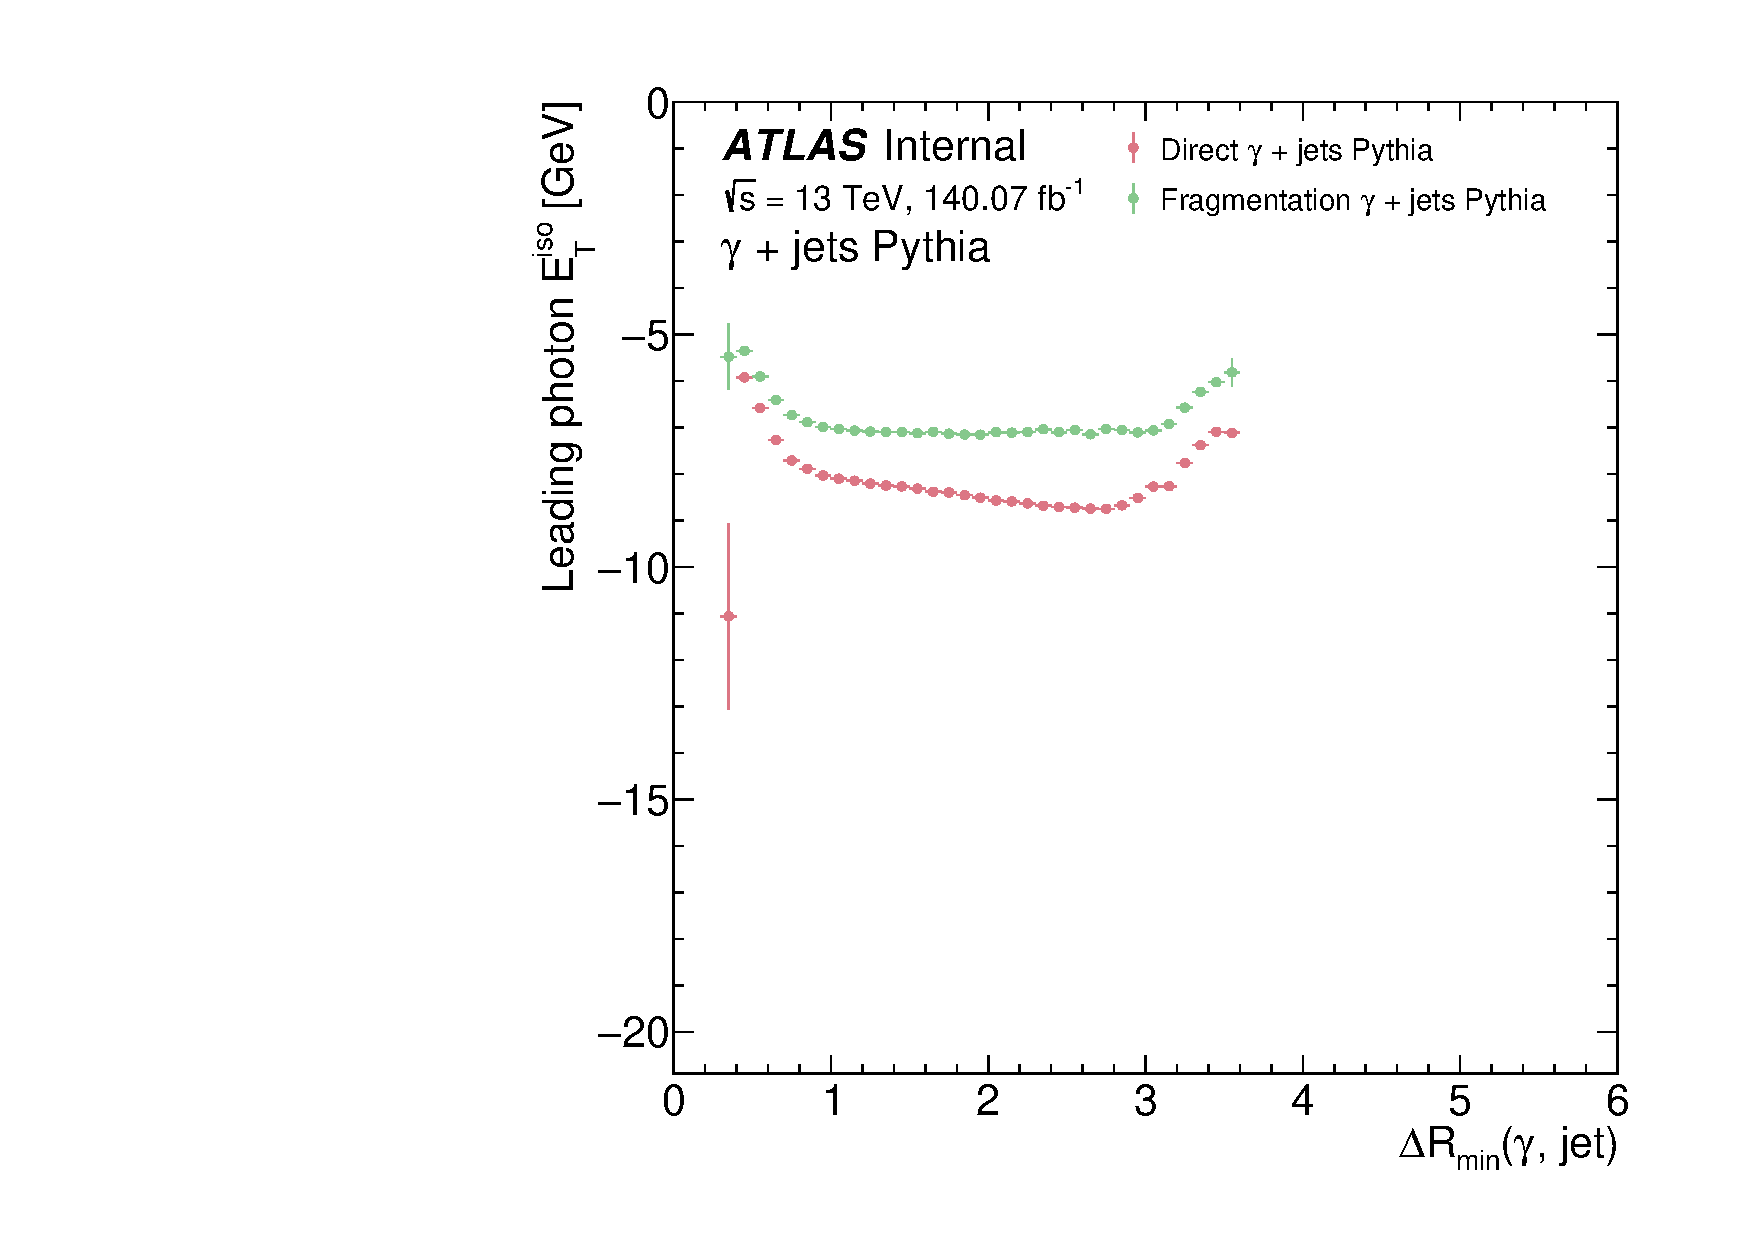
\includegraphics[width=\linewidth]{5_resonances/event_selection/extended_iso/can__photonjet_Pythia__phjet_drmin_ph_caloiso0__presel_deta_etas__Run2}
        \caption{Direct and fragmentation contributions separately.}
        \label{fig:evt_selection:sr_opt:extended_iso:phjet_drmin:etiso:separated}
    \end{subfigure}
    \caption{\(\etiso\) contribution as a function of \(\DeltaR_{\text{min}}\). The \etiso values are obtained from the mean of the \etiso distribution.}
    \label{fig:evt_selection:sr_opt:extended_iso:phjet_drmin:etiso}
\end{figure}

To study the contribution to the isolation energy of the photon from these jets, \Fig{\ref{fig:evt_selection:sr_opt:extended_iso:phjet_drmin:etiso:full}} shows the mean photon isolation energy contribution from the closest jet to the photon. Jets lying very close to the photon contribute highly to this energy, specially jets with \(\DeltaR (\gamma, j) < 1.0\), and in this particular value, the energy starts to drastically increase. This behaviour is also presented separately for direct and fragmentation photon production in \Fig{\ref{fig:evt_selection:sr_opt:extended_iso:phjet_drmin:etiso:separated}}, from which the higher contribution to the energy is given by fragmentation photon events.
From hereinafter, a cut to this variable at \(\DeltaR (\gamma, j) \geq 1.0\) is going to be considered to reduce fragmentation events and to obtain a cleaner photon signature.






\subsection{Jet \texorpdfstring{\pt}{pT}}
\label{subsec:evt_selection:sr_opt:jet_pt}


After applying all the aforementioned cuts, one observed, key, feature of fragmentation events is that there is a big proportion of events in which the leading jet carries much more momentum than the leading photon. In an ideal direct photon production, which is what is aimed to using this event selection, both the photon and jet carry approximately the same \pt. In order to study if a selection based on the jet and photon \pt is feasible, \ptgam vs \ptjet distributions are shown in \Fig{\ref{fig:evt_selection:sr_opt:jet_pt:ptgam_ptjet}} for both direct and fragmentation photons. From these figures, it can be clearly seen that the fragmentation photon production is the one contributing to having events with \(\ptjet \gg \ptgam\).


\begin{figure}[ht!]
    \centering
    \begin{subfigure}[h]{0.49\linewidth}
        \centering
        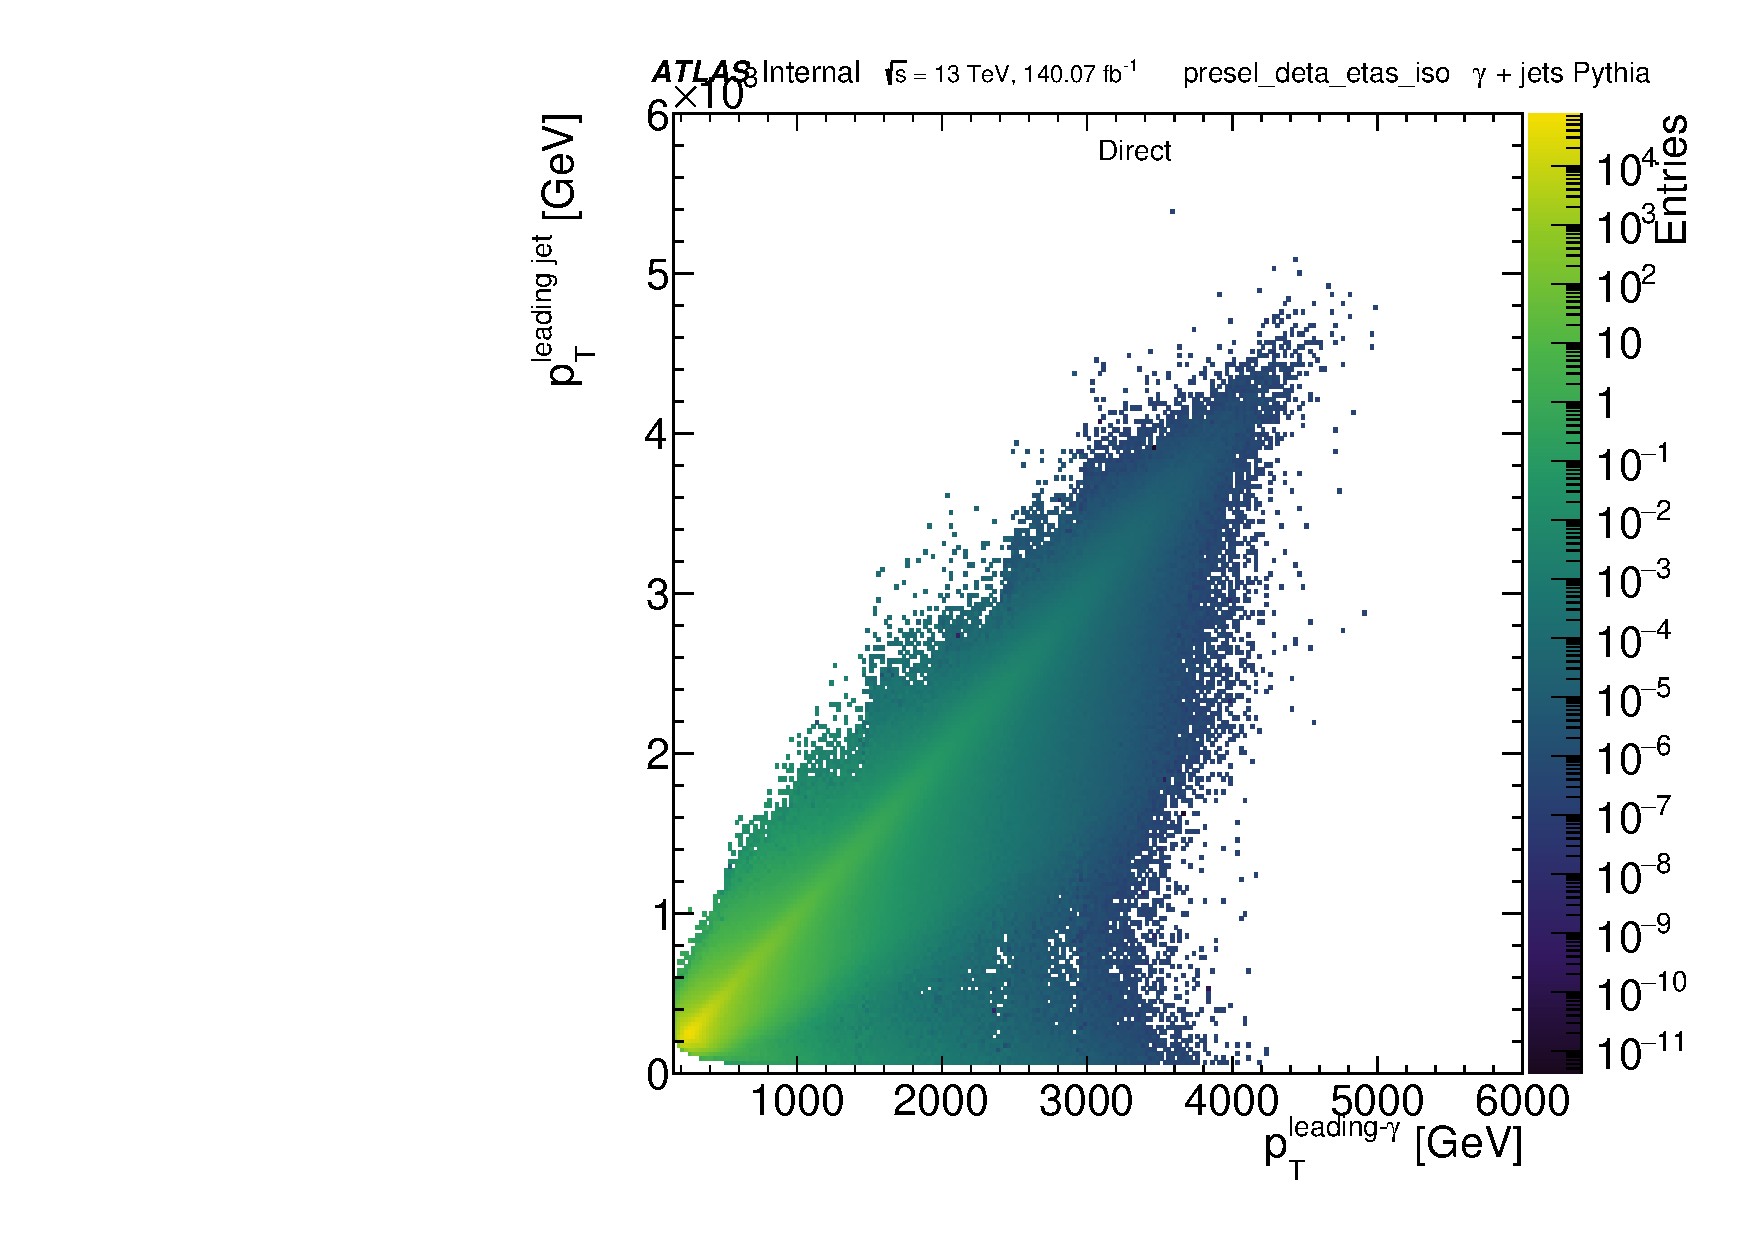
\includegraphics[width=\linewidth]{5_resonances/event_selection/jet_pt/presel_deta_etas_iso/bkg/2d/can2d__direct__presel_deta_etas_iso__ph_pt0_jet_pt0}
        \caption{Direct photons}
    \end{subfigure}
    \hfill
    \begin{subfigure}[h]{0.49\linewidth}
        \centering
        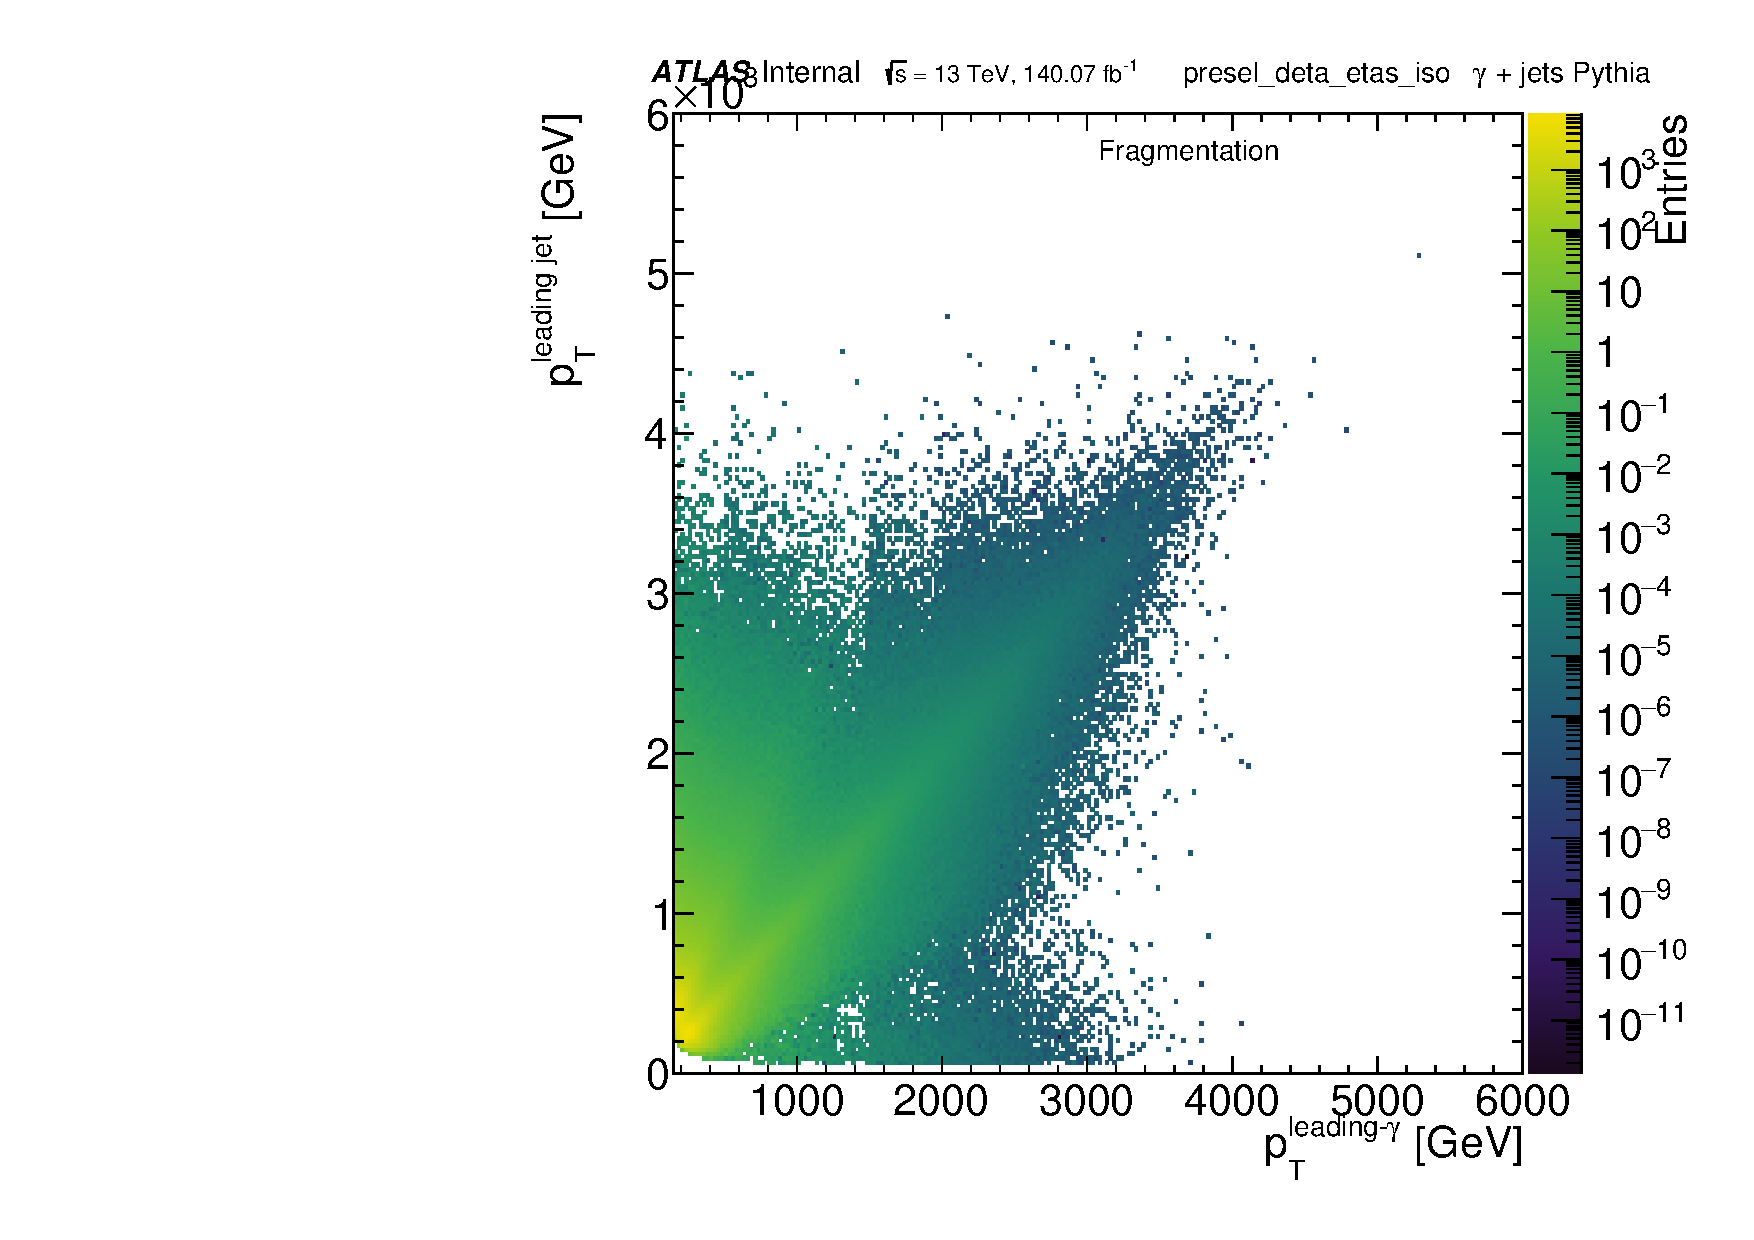
\includegraphics[width=\linewidth]{5_resonances/event_selection/jet_pt/presel_deta_etas_iso/bkg/2d/can2d__fragmentation__presel_deta_etas_iso__ph_pt0_jet_pt0}
        \caption{Fragmentation photons}
    \end{subfigure}
    \caption{\ptgam-\ptjet 2D distribution for direct and fragmentation \pythia \gammajet background.}
    \label{fig:evt_selection:sr_opt:jet_pt:ptgam_ptjet}
\end{figure}

\begin{figure}[ht!]
    \centering
    \begin{subfigure}[h]{0.49\linewidth}
        \centering
        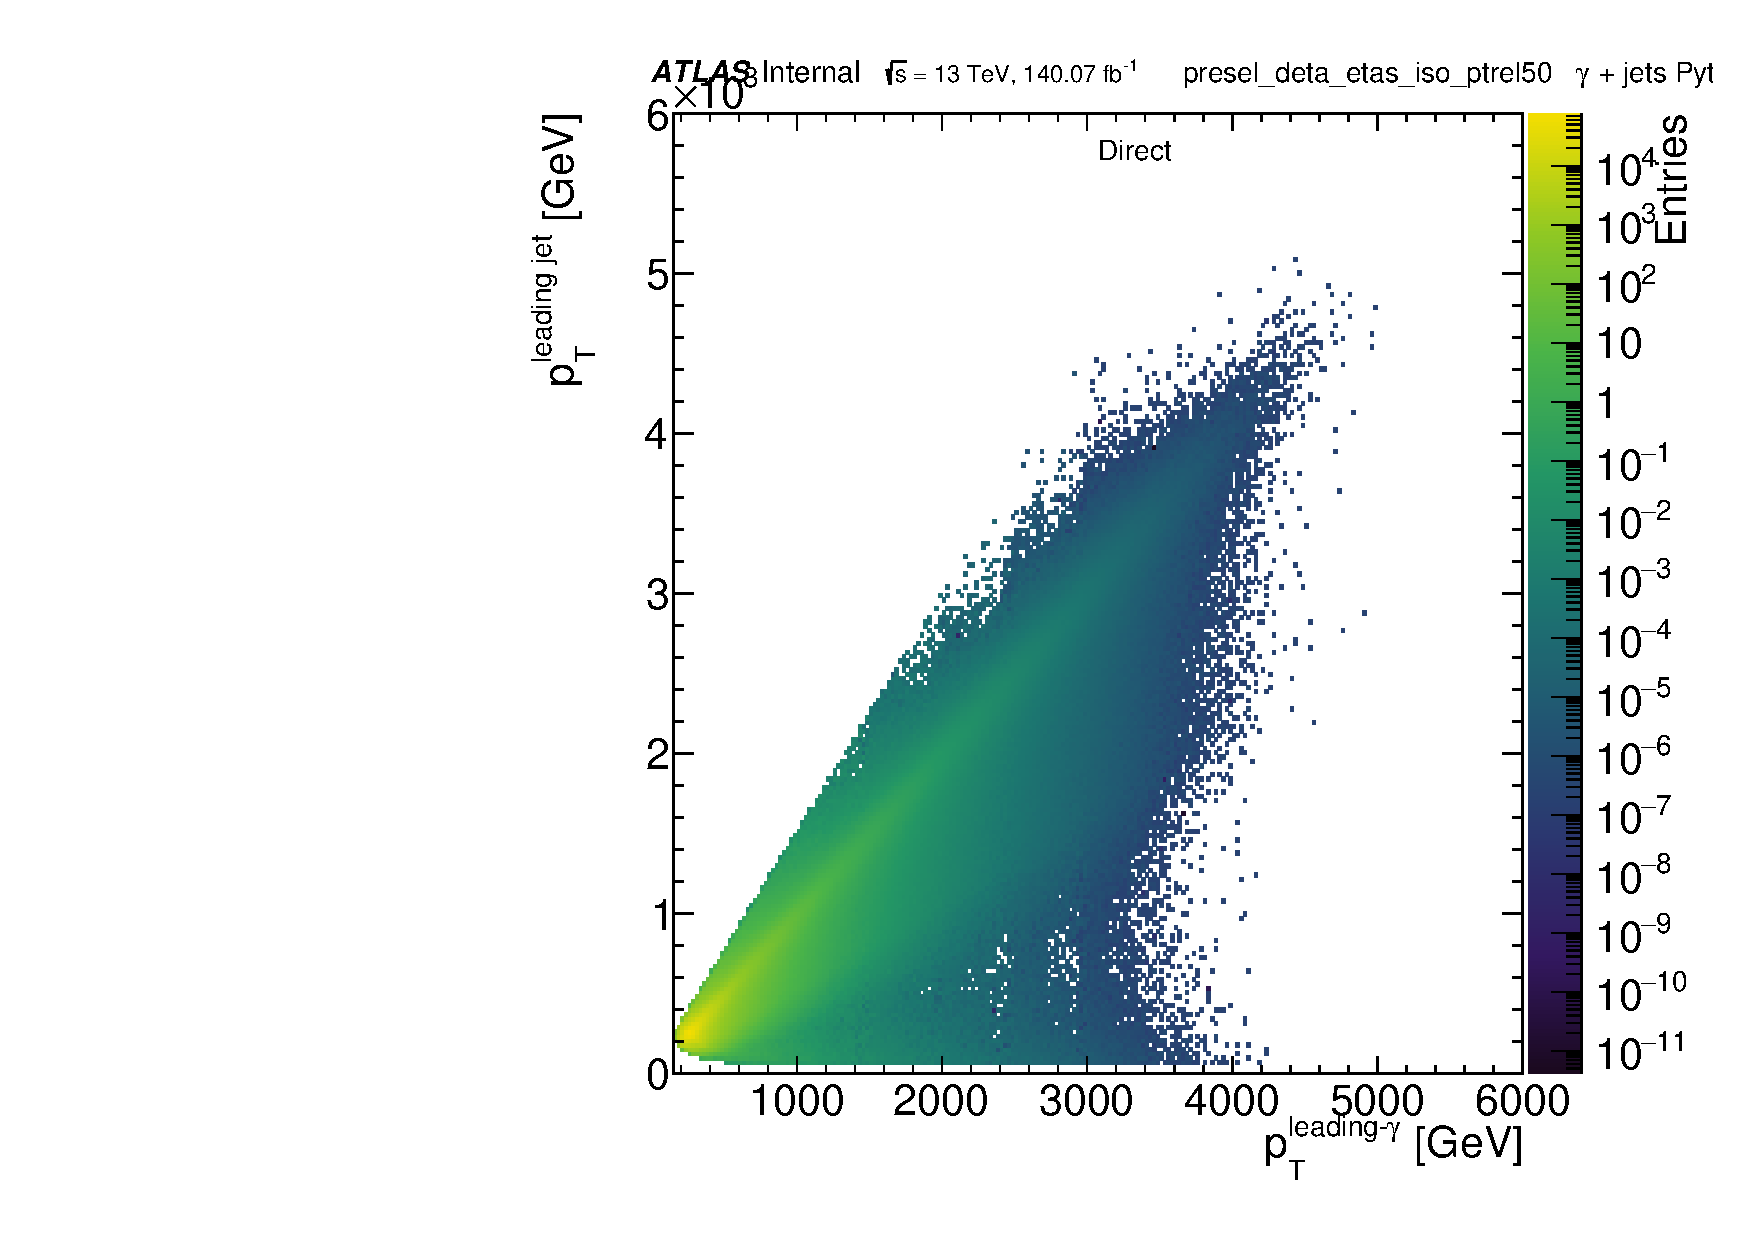
\includegraphics[width=\linewidth]{5_resonances/event_selection/jet_pt/presel_deta_etas_iso_ptrel50/bkg/2d/can2d__direct__presel_deta_etas_iso_ptrel50__ph_pt0_jet_pt0}
        \caption{Direct photons}
    \end{subfigure}
    \hfill
    \begin{subfigure}[h]{0.49\linewidth}
        \centering
        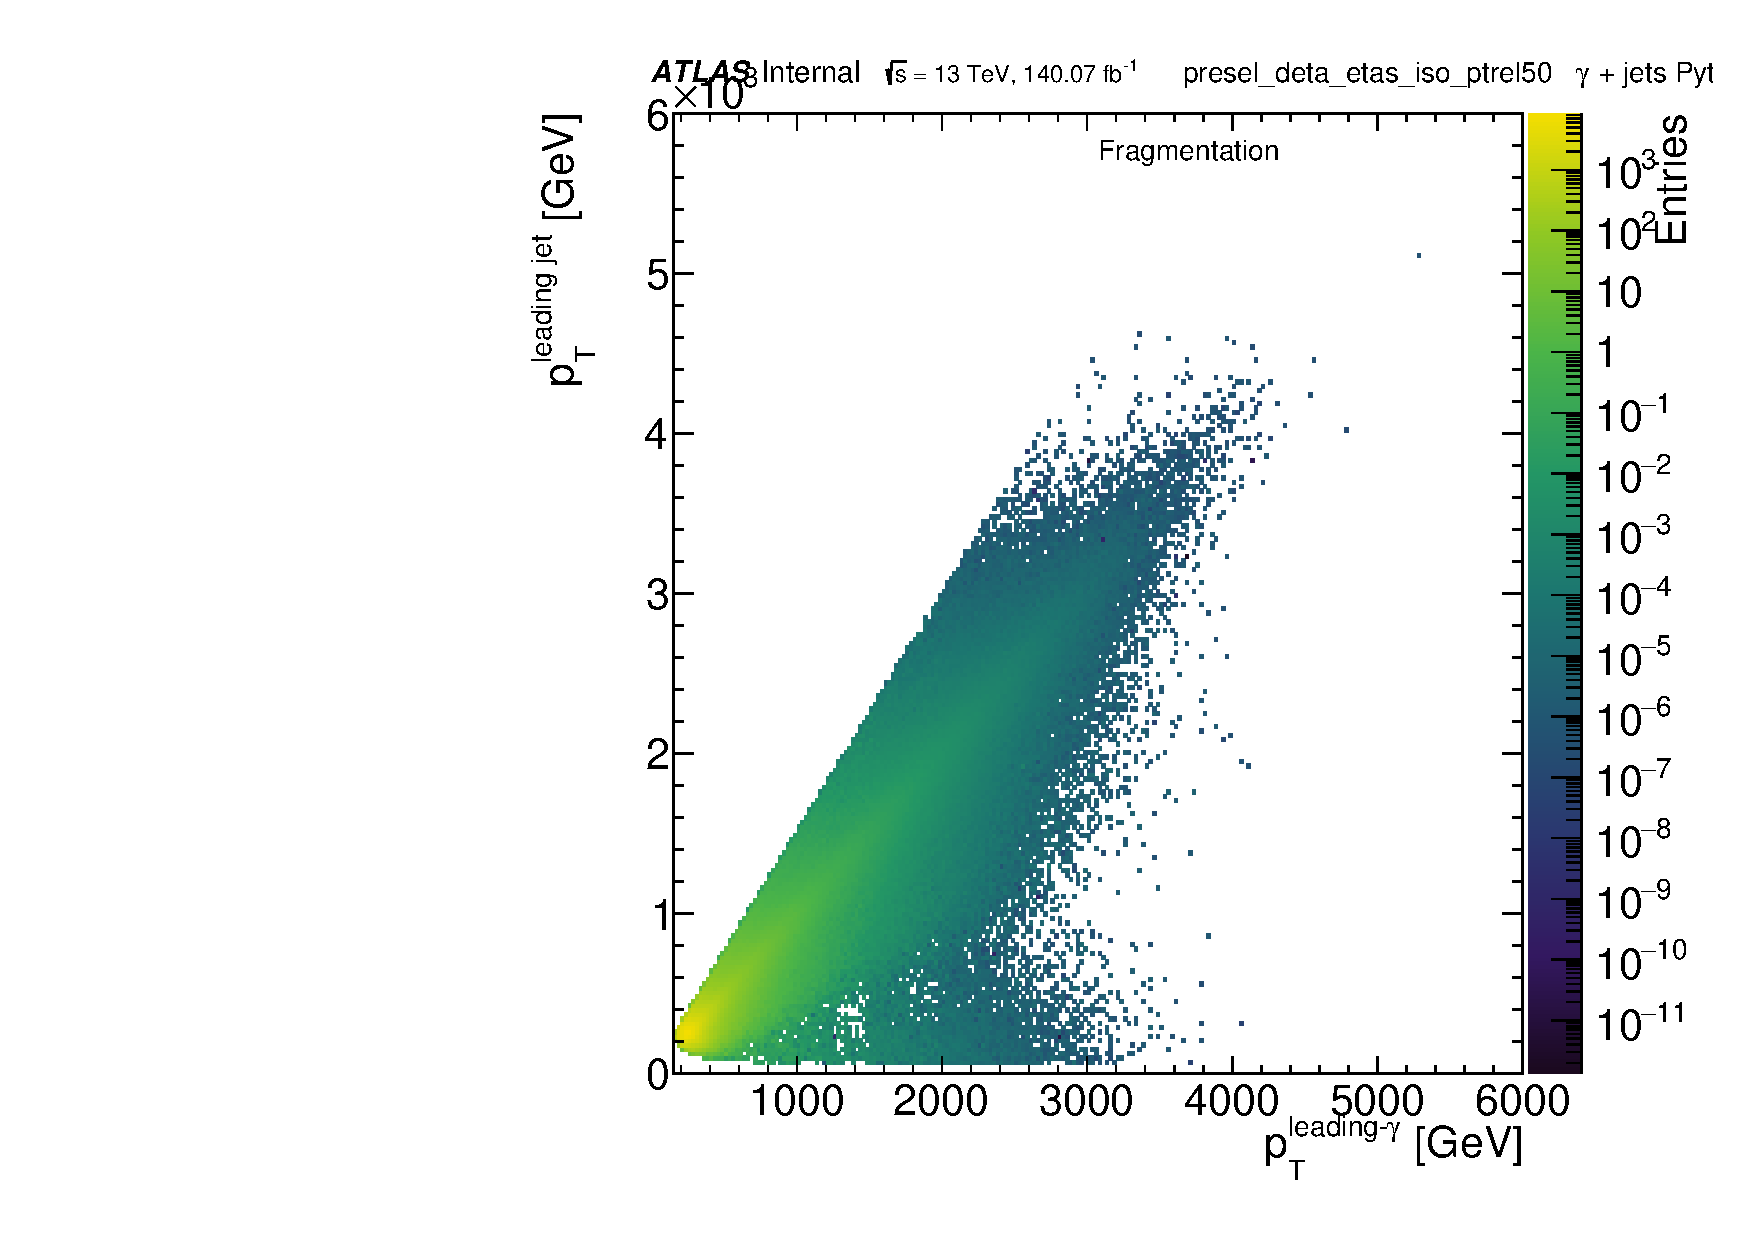
\includegraphics[width=\linewidth]{5_resonances/event_selection/jet_pt/presel_deta_etas_iso_ptrel50/bkg/2d/can2d__fragmentation__presel_deta_etas_iso_ptrel50__ph_pt0_jet_pt0}
        \caption{Fragmentation photons}
    \end{subfigure}
    \caption{\ptgam-\ptjet 2D distribution for direct and fragmentation \pythia \gammajet background, selecting events in which the leading jet \pt satisfies \Eqn{\ref{eq:evt_selection:sr_opt:jet_pt:jet_pt_rel_X}} with \(X=0.5\).}
    \label{fig:evt_selection:sr_opt:jet_pt:ptgam_ptjet_X0.5}
\end{figure}



In order to clean the sample from fragmentation photon contributions even more, the events selected are those that satisfy:
\begin{equation}
    \label{eq:evt_selection:sr_opt:jet_pt:jet_pt_rel_X}
    \frac{\ptjet - \ptgam}{\ptgam} < X, \qquad X \in [0, 1]
\end{equation}
where \(X\) is the allowed fraction of \ptgam the jet has to have, hence defining an upper value for \ptjet for a given \ptgam. The optimal value is found to be \(X=0.5\), at which the signal efficiency is very high, while the rejected background consists solely of fragmentation events.

In \Fig{\ref{fig:evt_selection:sr_opt:jet_pt:ptgam_ptjet_X0.5}}, the background \ptgam vs \ptjet distribution is shown again separately for direct and fragmentation photons, from which it is noted that the vast majority of events removed are fragmentation. The same distribution for different \ac{EQ} signals is shown in \Fig{\ref{fig:evt_selection:sr_opt:jet_pt:ptgam_ptjet_signals}}, having efficiencies greater than 95\%. The cut efficiency for background and some \qstar signals are shown in \Tab{\ref{tab:evt_selection:sr_opt:jet_pt:efficiency_selection}}.


\begin{figure}[ht!]
    \centering
    \begin{subfigure}[h]{0.32\linewidth}
        \centering
        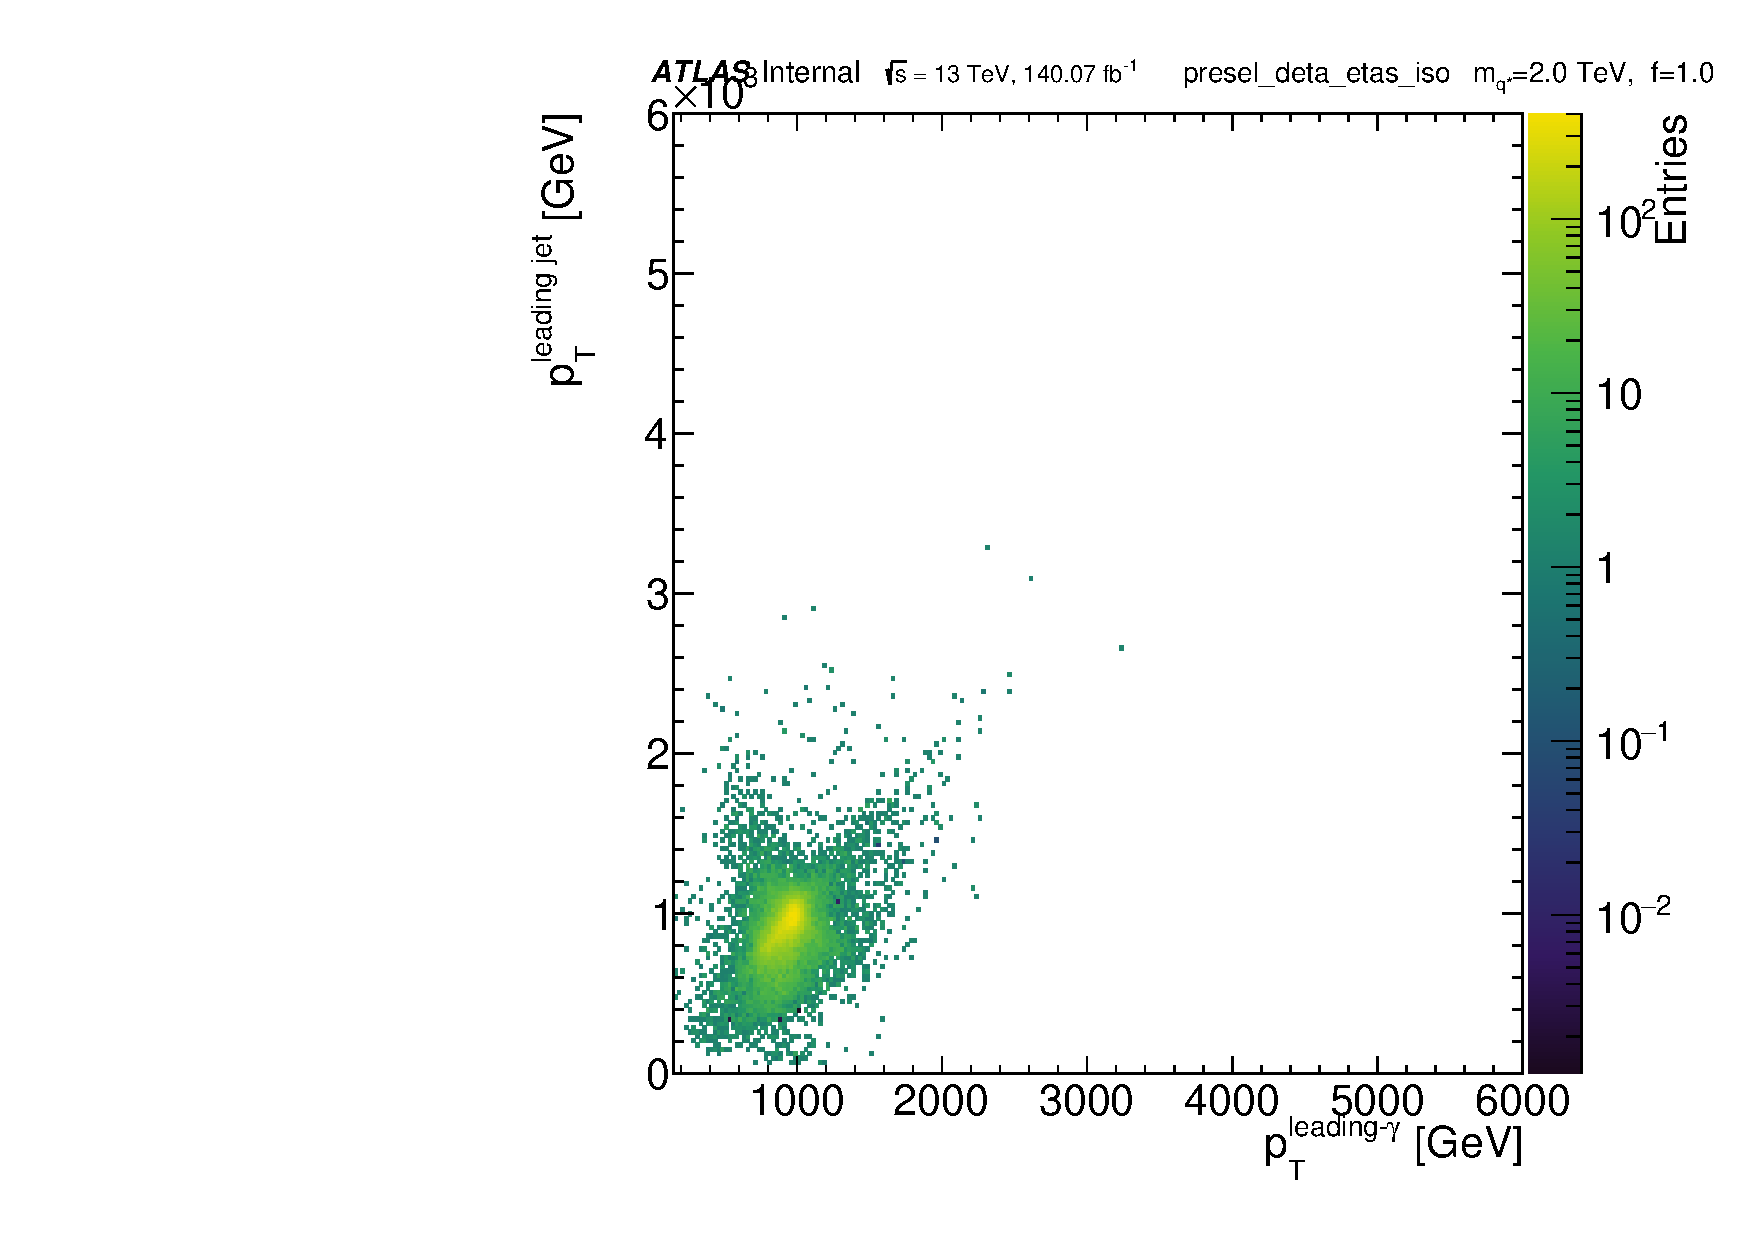
\includegraphics[width=\linewidth]{5_resonances/event_selection/jet_pt/presel_deta_etas_iso/sig/2d/can2d__qStar_f1p00_M2000__presel_deta_etas_iso__ph_pt0_jet_pt0}
        \caption{\(\mq=2000~\gev\).}
    \end{subfigure}
    \hfill
    \begin{subfigure}[h]{0.32\linewidth}
        \centering
        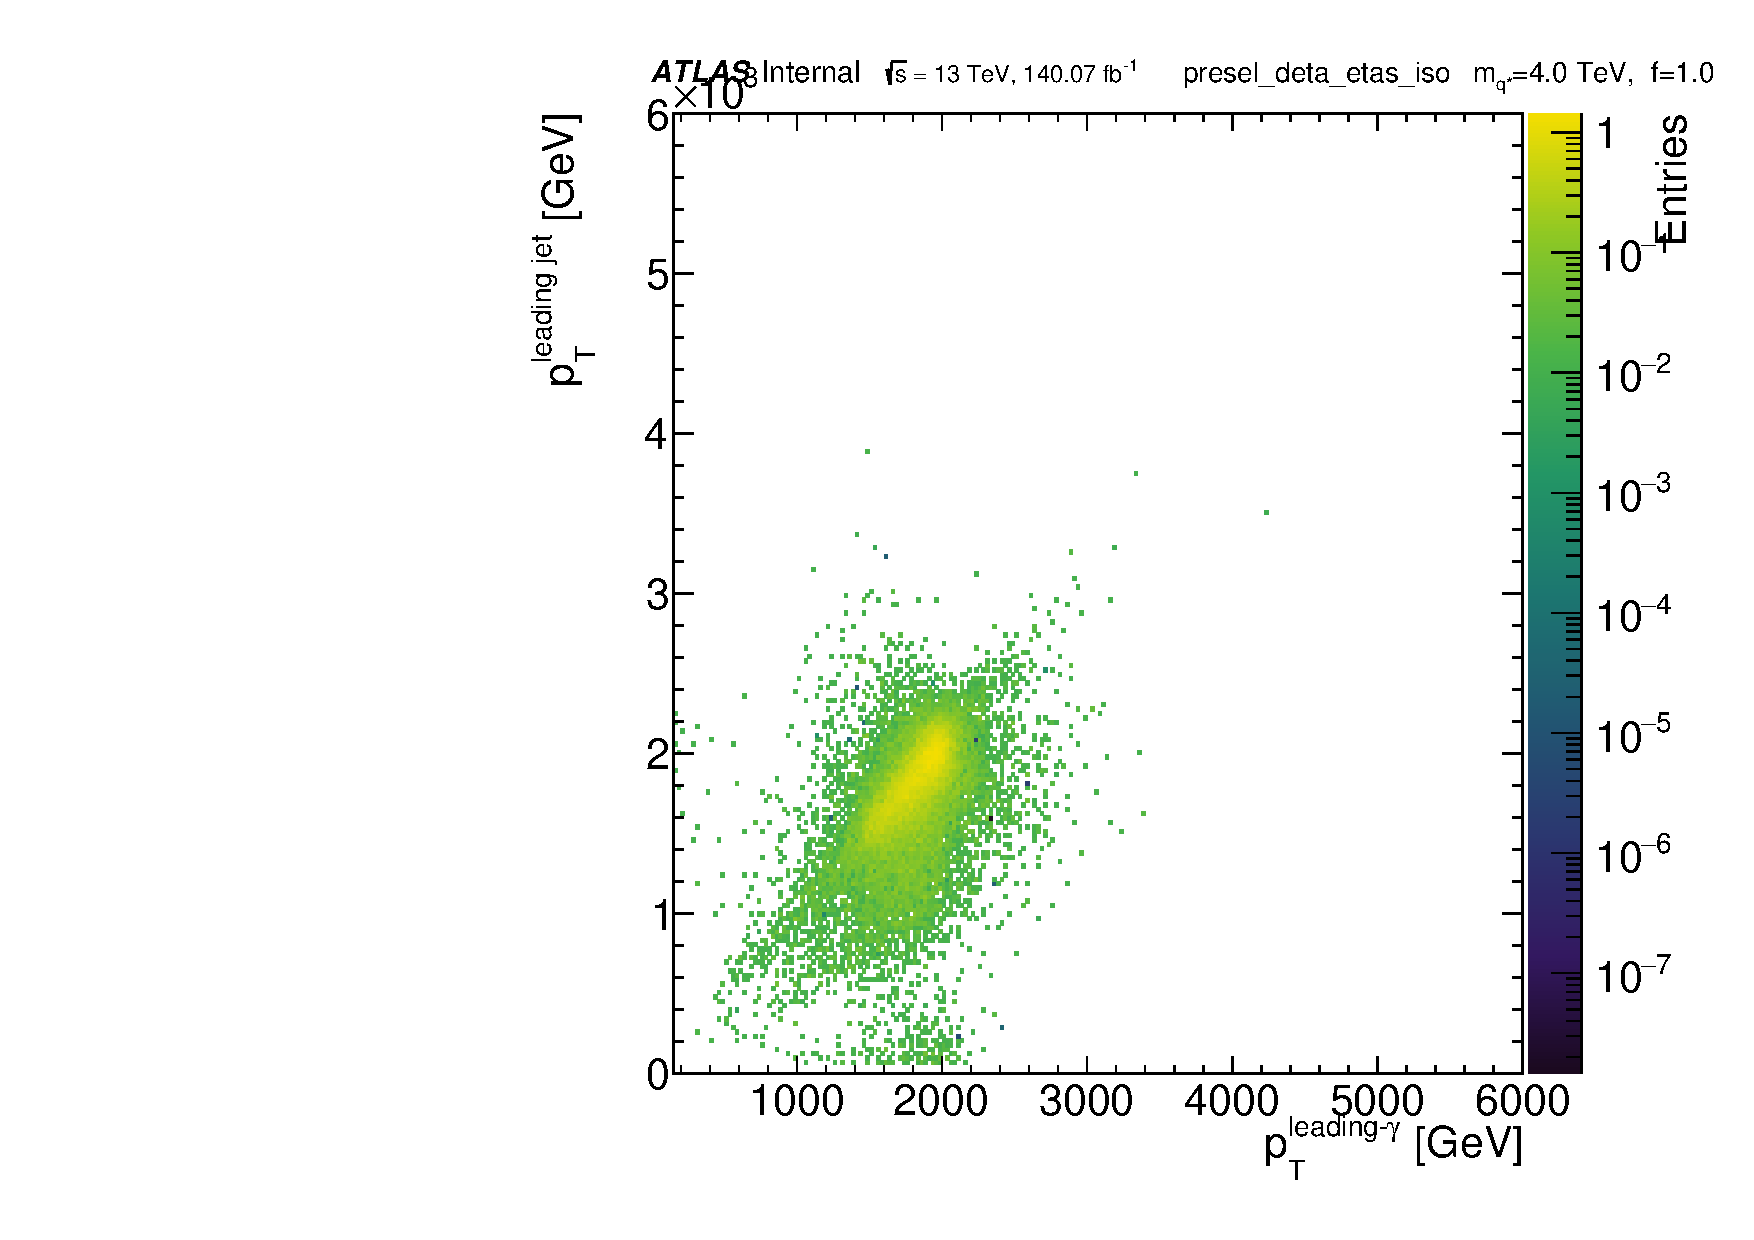
\includegraphics[width=\linewidth]{5_resonances/event_selection/jet_pt/presel_deta_etas_iso/sig/2d/can2d__qStar_f1p00_M4000__presel_deta_etas_iso__ph_pt0_jet_pt0}
        \caption{\(\mq=4000~\gev\).}
    \end{subfigure}
    \hfill
    \begin{subfigure}[h]{0.32\linewidth}
        \centering
        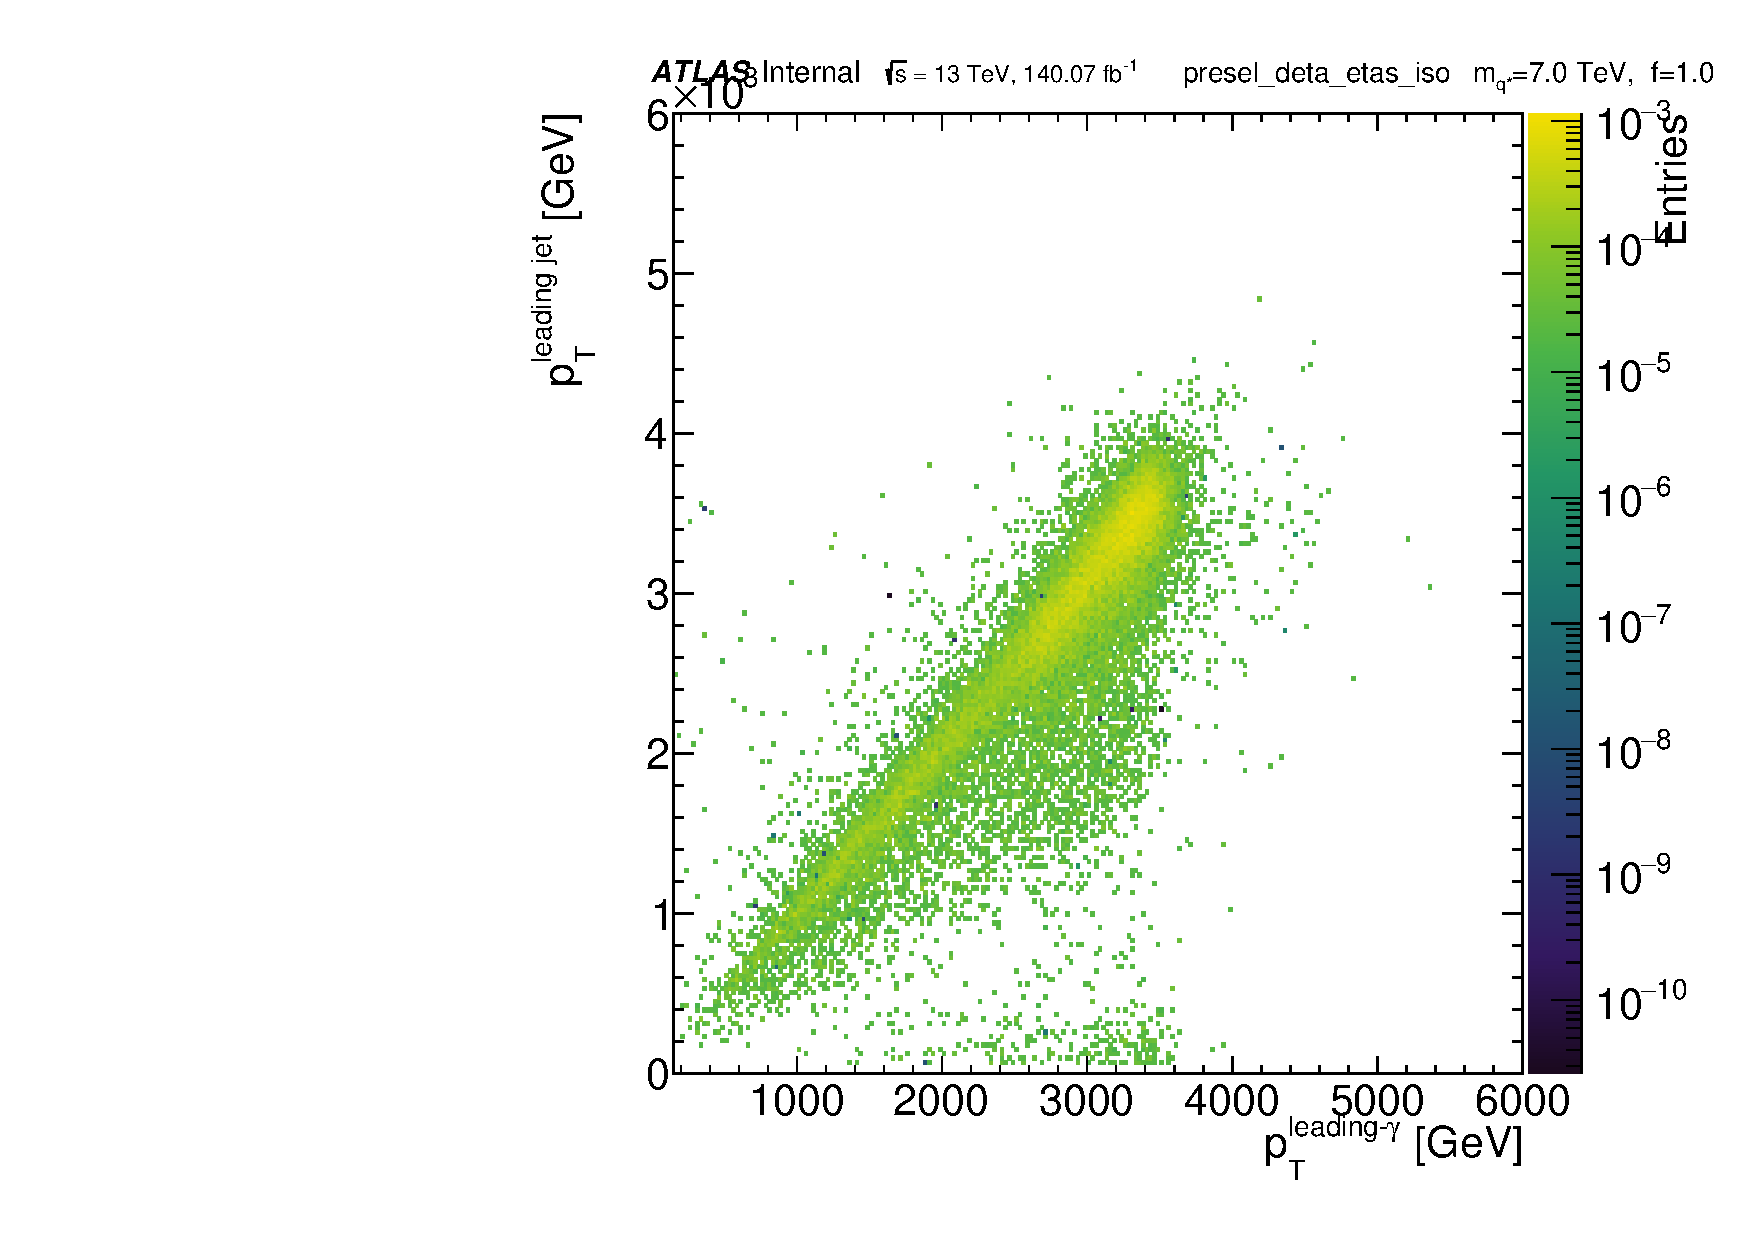
\includegraphics[width=\linewidth]{5_resonances/event_selection/jet_pt/presel_deta_etas_iso/sig/2d/can2d__qStar_f1p00_M7000__presel_deta_etas_iso__ph_pt0_jet_pt0}
        \caption{\(\mq=7000~\gev\).}
    \end{subfigure}\\
    \begin{subfigure}[h]{0.32\linewidth}
        \centering
        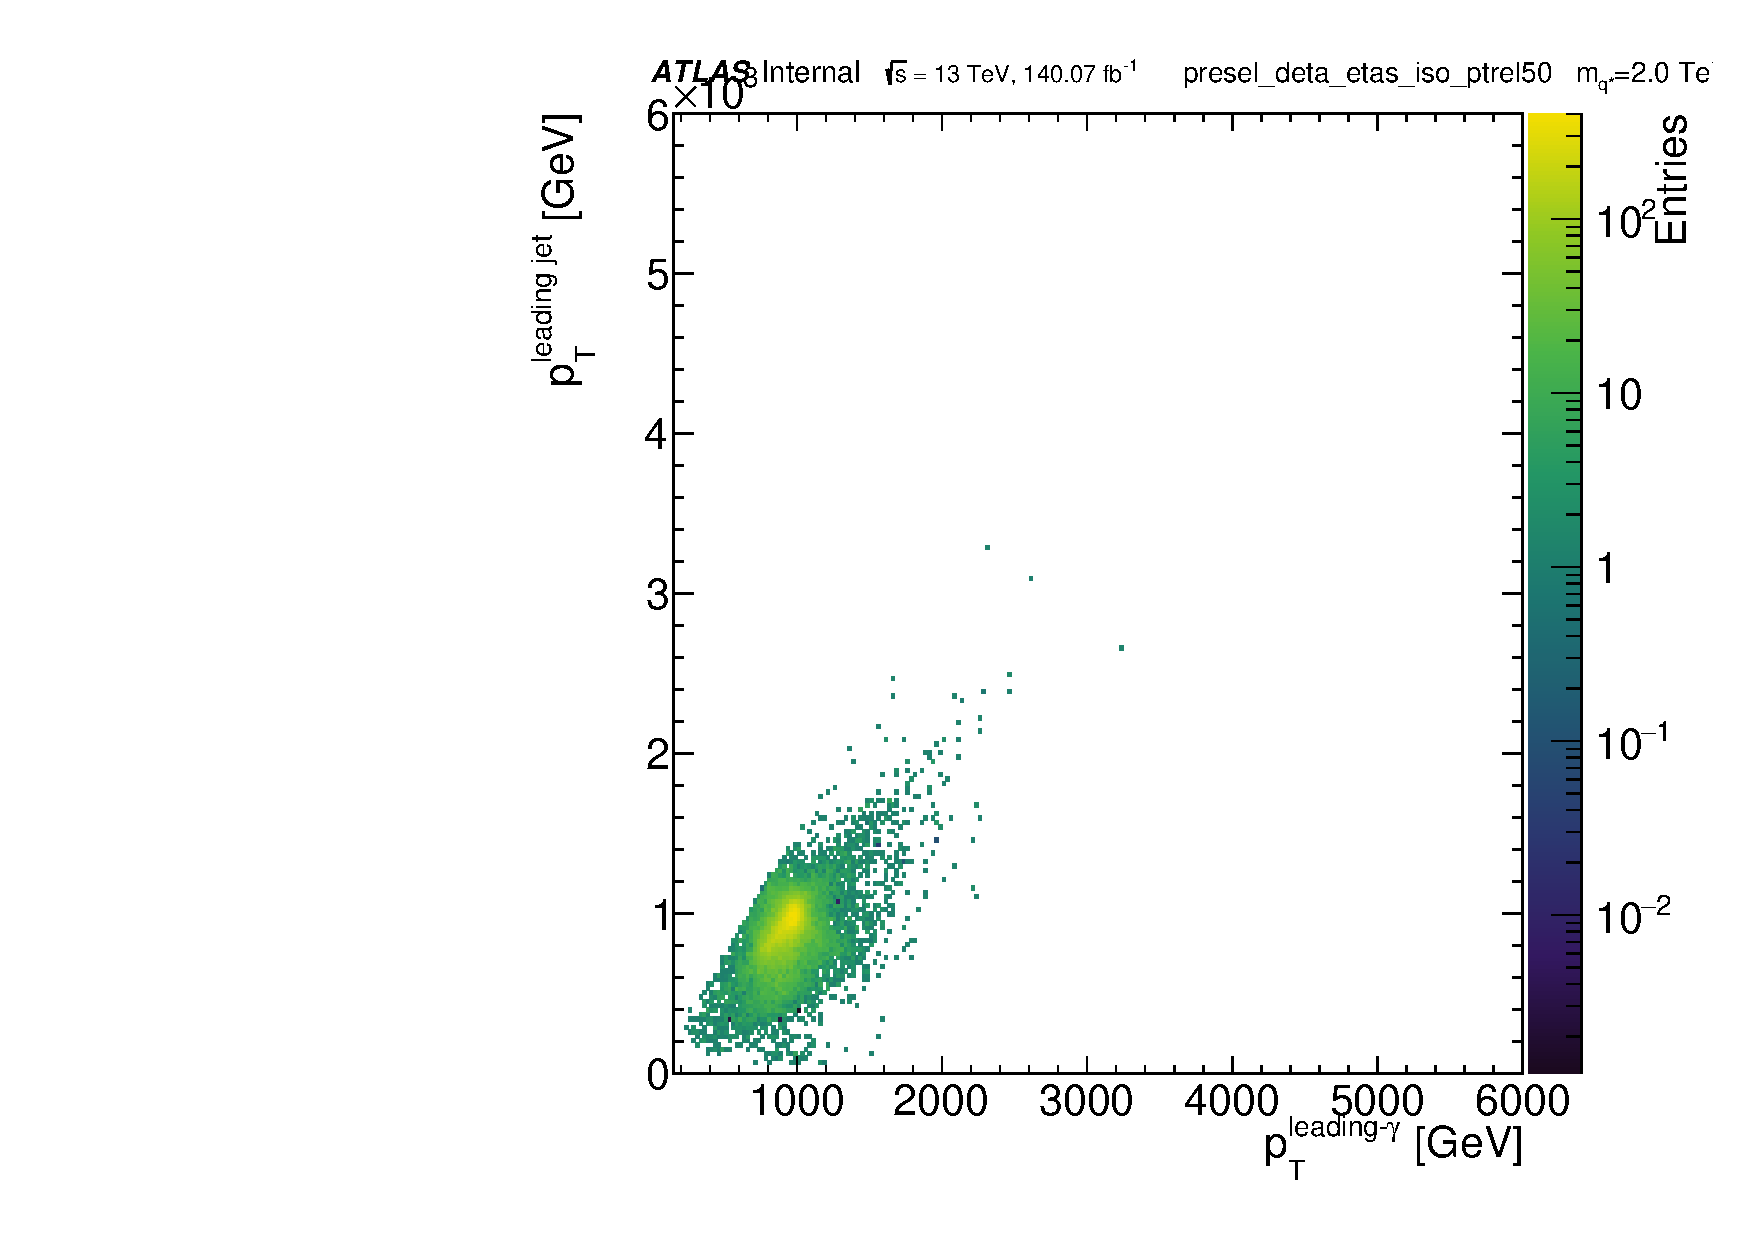
\includegraphics[width=\linewidth]{5_resonances/event_selection/jet_pt/presel_deta_etas_iso_ptrel50/sig/2d/can2d__qStar_f1p00_M2000__presel_deta_etas_iso_ptrel50__ph_pt0_jet_pt0}
        \caption{\(\mq=2000~\gev\), \ptjet cut applied.}
    \end{subfigure}
    \hfill
    \begin{subfigure}[h]{0.32\linewidth}
        \centering
        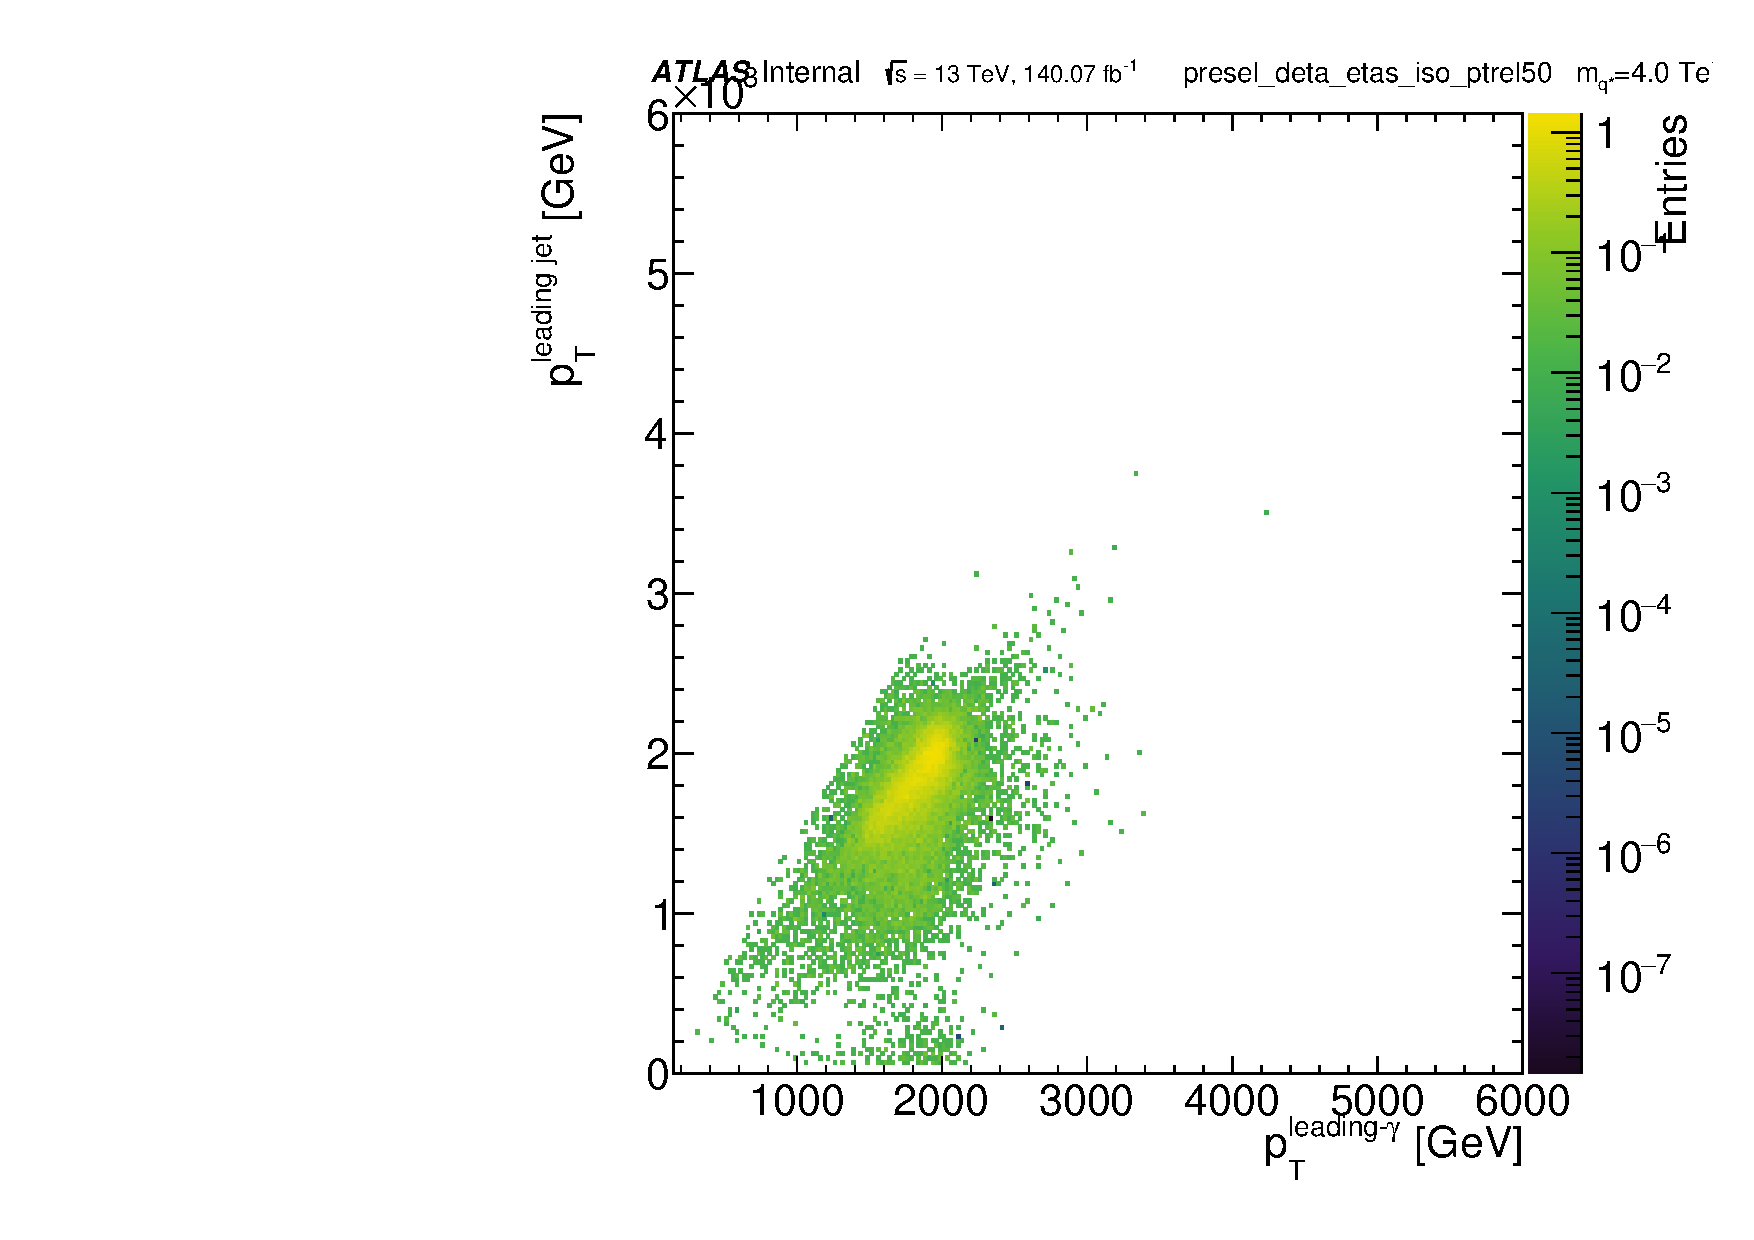
\includegraphics[width=\linewidth]{5_resonances/event_selection/jet_pt/presel_deta_etas_iso_ptrel50/sig/2d/can2d__qStar_f1p00_M4000__presel_deta_etas_iso_ptrel50__ph_pt0_jet_pt0}
        \caption{\(\mq=4000~\gev\), \ptjet cut applied.}
    \end{subfigure}
    \hfill
    \begin{subfigure}[h]{0.32\linewidth}
        \centering
        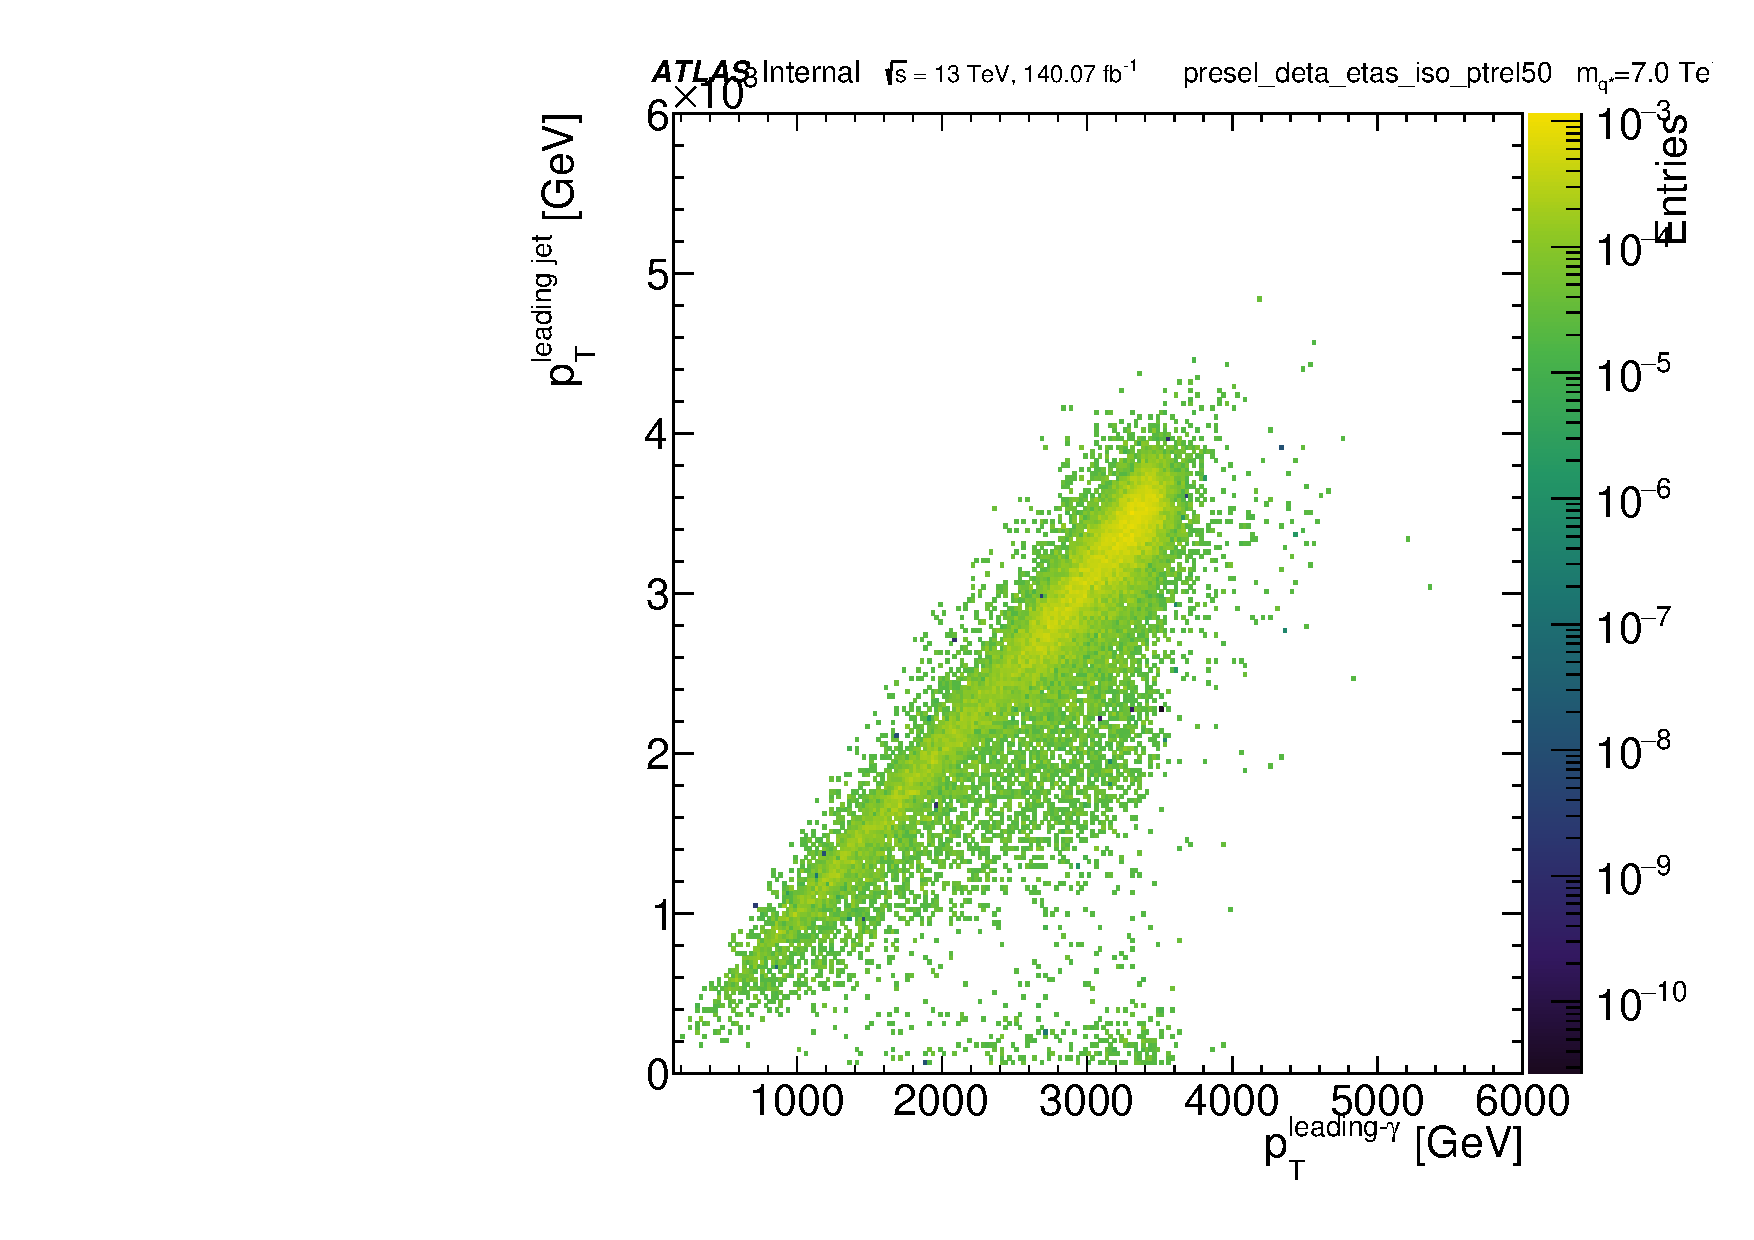
\includegraphics[width=\linewidth]{5_resonances/event_selection/jet_pt/presel_deta_etas_iso_ptrel50/sig/2d/can2d__qStar_f1p00_M7000__presel_deta_etas_iso_ptrel50__ph_pt0_jet_pt0}
        \caption{\(\mq=7000~\gev\), \ptjet cut applied.}
    \end{subfigure}\\
    \caption{\ptgam-\ptjet 2D distribution for different \qstar signal samples with \(f=1.0\), selecting jets according to formula \Eqn{\ref{eq:evt_selection:sr_opt:jet_pt:jet_pt_rel_X}} with \(X=0.5\). The first three figures shown the 2D distribution without the application of the \ptjet cut, while the three at the botton contain it.}
    \label{fig:evt_selection:sr_opt:jet_pt:ptgam_ptjet_signals}
\end{figure}



\begin{table}[ht!]
    \centering
    \caption{Background and signal efficiency on the \ptjet cut defined above.}
    \begin{tabular}{lc}
        \toprule
        & \(\varepsilon_{\text{rel}}\) \\
        \midrule
        \gammajet Pythia & $0.8827$ \\
        \(\mq=2000~\gev\),  \(f=1.00\) & $0.9707$ \\
        \(\mq=4000~\gev\),  \(f=1.00\) & $0.9918$ \\
        \(\mq=7000~\gev\),  \(f=1.00\) & $0.9942$ \\
        \bottomrule
    \end{tabular}
    \label{tab:evt_selection:sr_opt:jet_pt:efficiency_selection}
\end{table}



The variable that is affected the most by this particular cut is, as expected, \ptjet. This distribution is shown in \Fig{\ref{fig:evt_selection:sr_opt:jet_pt:jet_pt}} before and after the cut is applied. It is observed how the fragmentation events contribution drastically decrease, making the \ptjet distribution much smoother. Moreover, since the observable of interest is \myj, a comparison of this distribution is shown in \Fig{\ref{fig:evt_selection:sr_opt:jet_pt:phjet_m}}, to assess the changes in the spectrum. Applying this particular cut on \ptjet has almost not effect on the final \myj distribution. Very small differences are observed but at very low \myj. This is due to the asymmetry in \pt that the jet and photon had (\(\ptjet \gg \ptgam\)).

In the final selection, the cut \((\ptjet - \ptgam) / \ptgam < 0.5\) is applied.

\begin{figure}[ht!]
    \centering
    \begin{subfigure}[h]{0.32\linewidth}
        \centering
        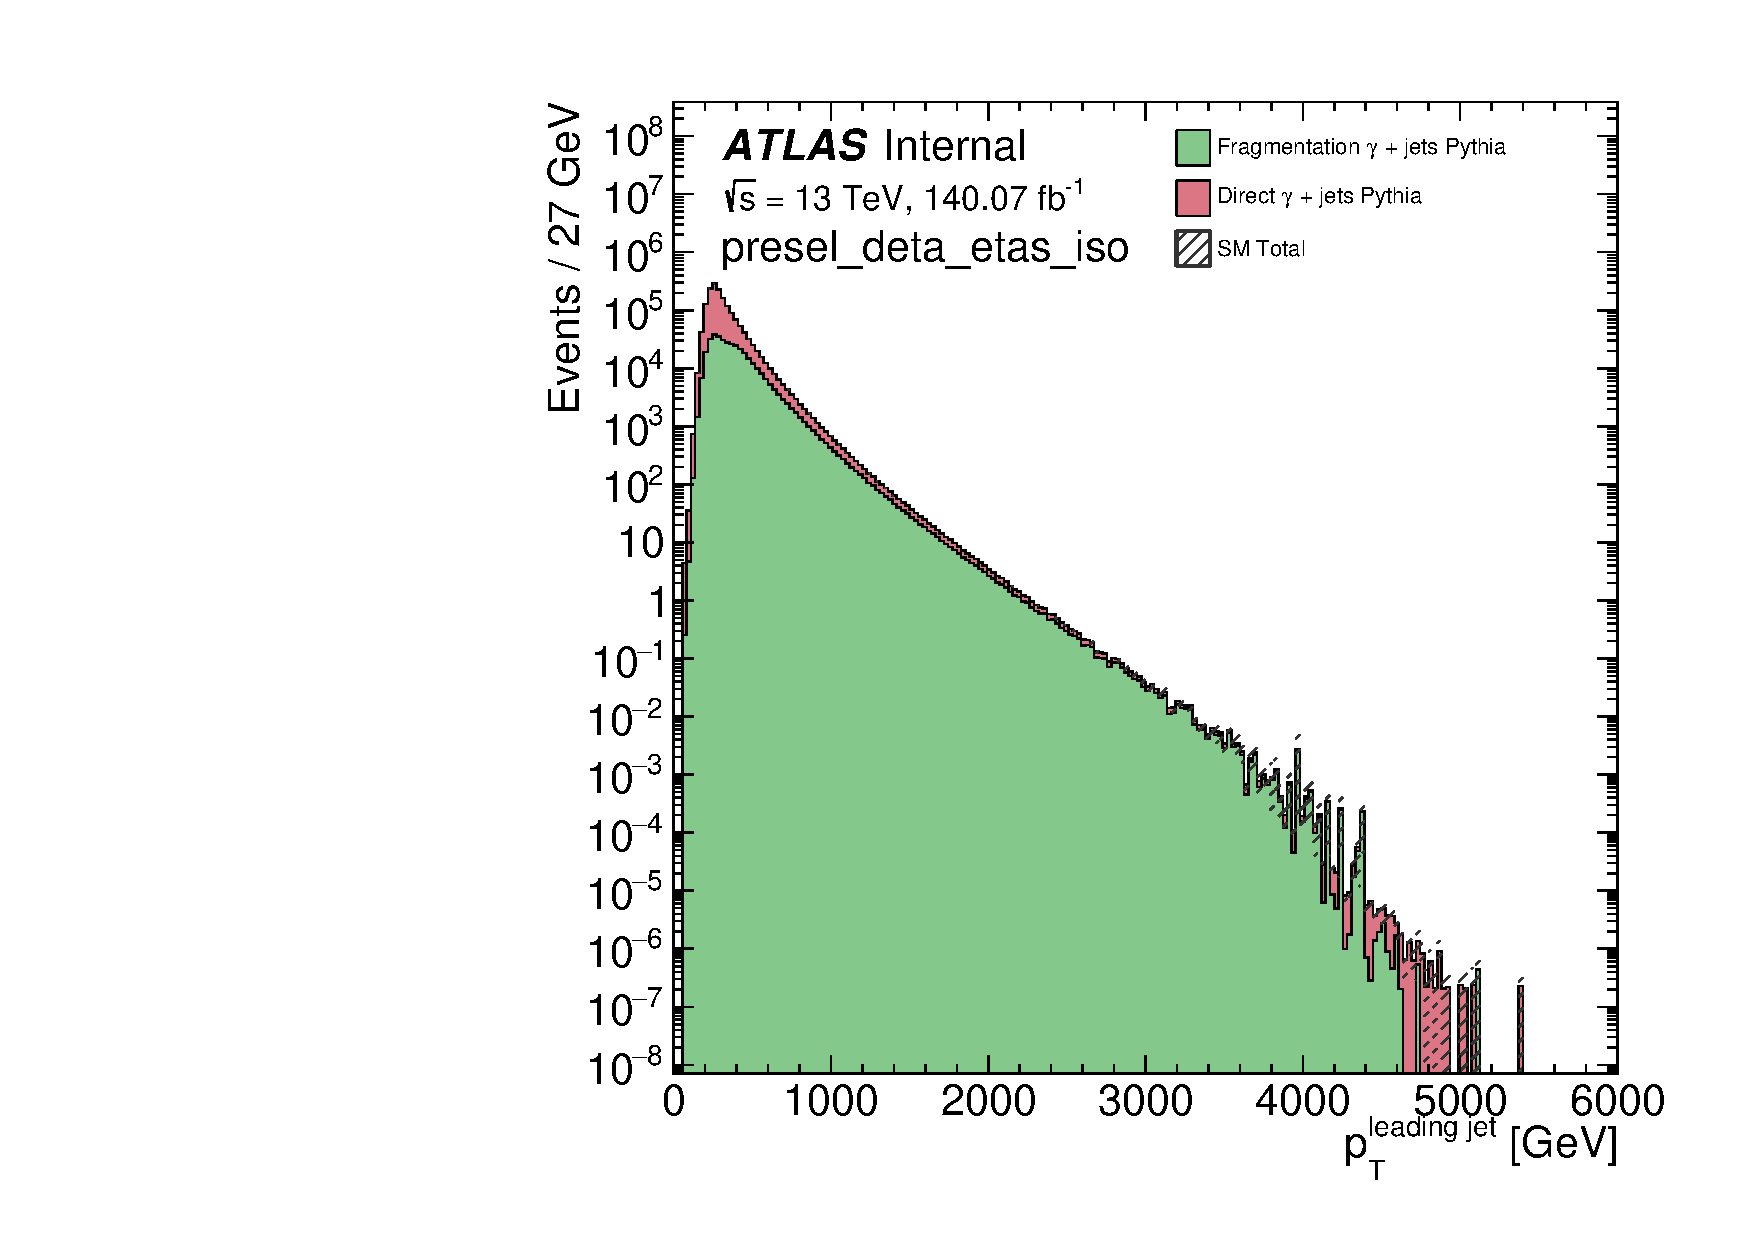
\includegraphics[width=\linewidth]{5_resonances/event_selection/jet_pt/presel_deta_etas_iso/bkg/1d/no_normalized/can__photonjet_Pythia__presel_deta_etas_iso__jet_pt0__Run2}
        \caption{Before \ptjet cut.}
    \end{subfigure}
    \hfill
    \begin{subfigure}[h]{0.32\linewidth}
        \centering
        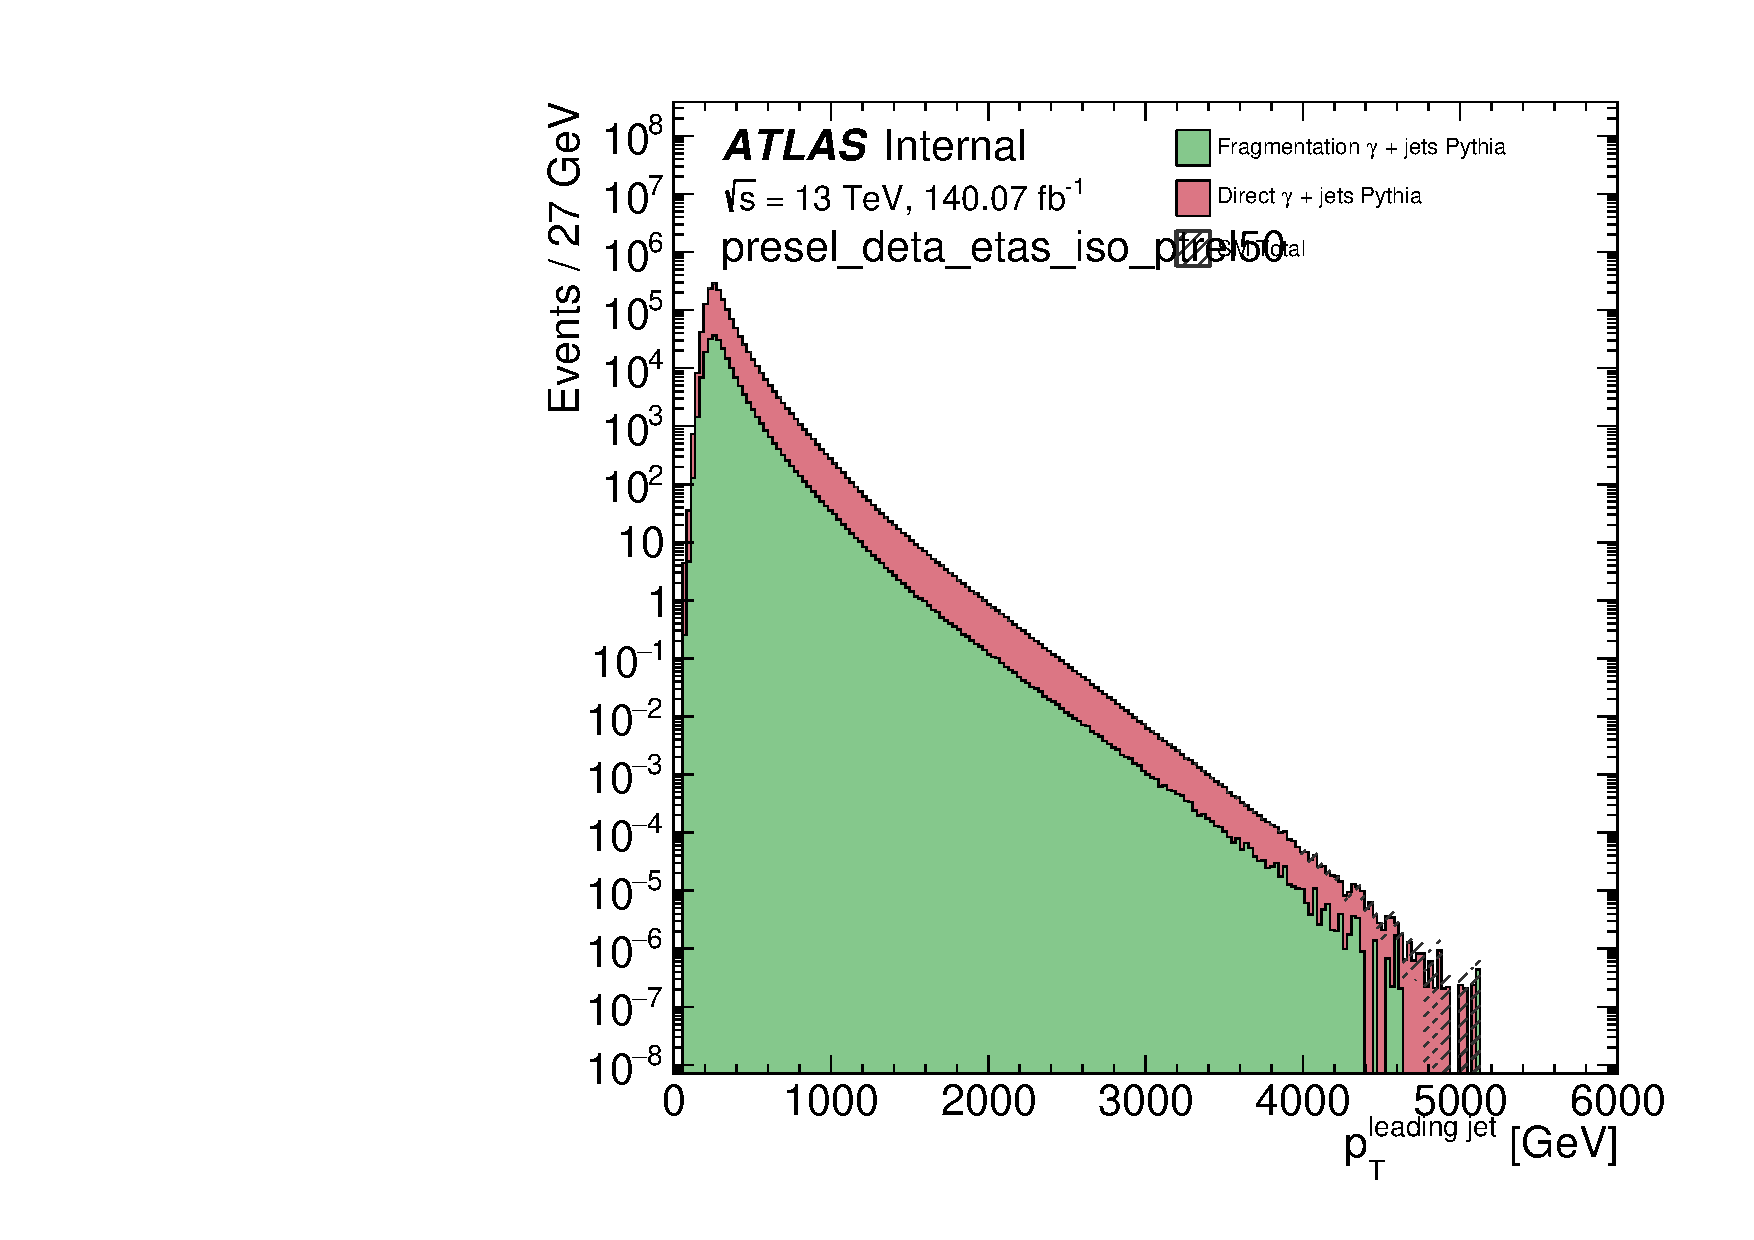
\includegraphics[width=\linewidth]{5_resonances/event_selection/jet_pt/presel_deta_etas_iso_ptrel50/bkg/1d/no_normalized/can__photonjet_Pythia__presel_deta_etas_iso_ptrel50__jet_pt0__Run2}
        \caption{After \ptjet cut.}
    \end{subfigure}
    \hfill
    \begin{subfigure}[h]{0.32\linewidth}
        \centering
        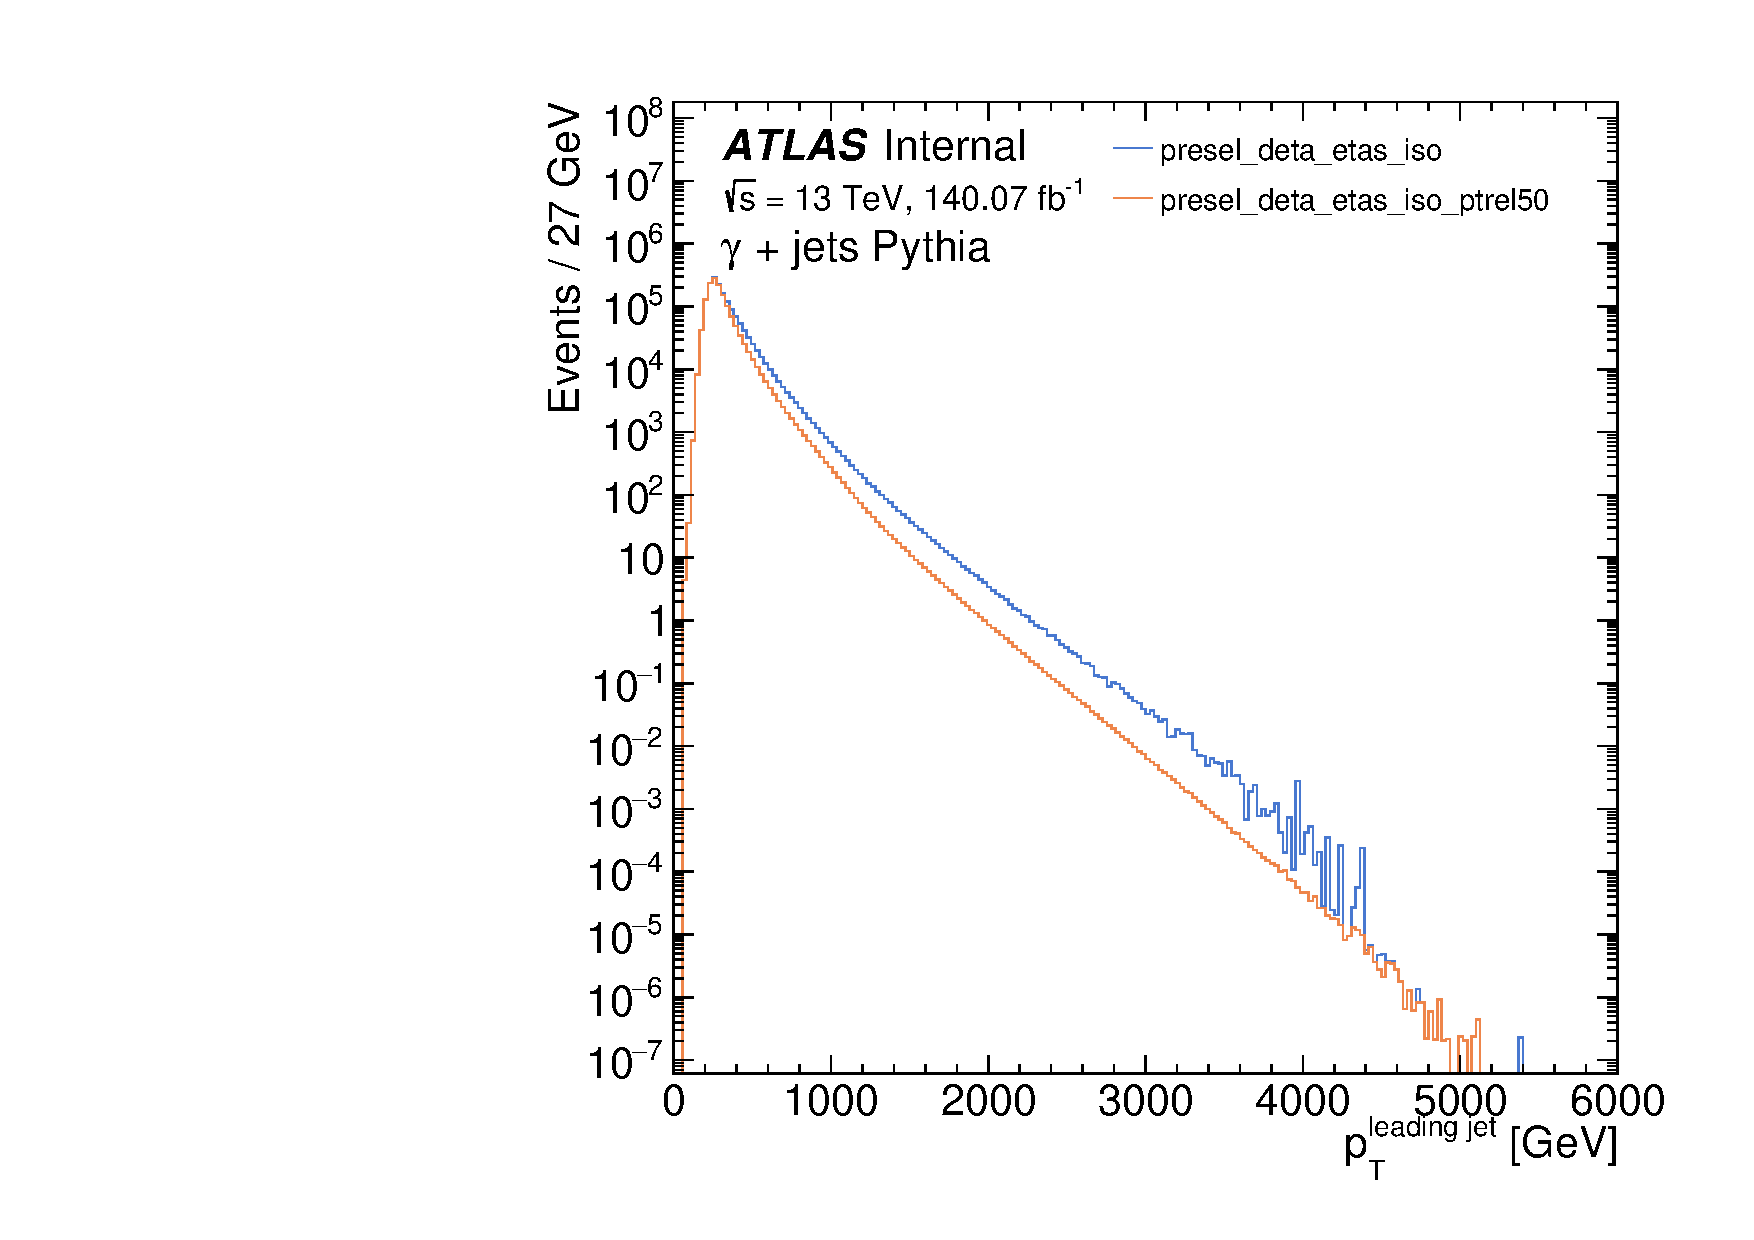
\includegraphics[width=\linewidth]{5_resonances/event_selection/jet_pt/can__photonjet_Pythia__jet_pt0__regions_presel_deta_etas_iso_presel_deta_etas_iso_ptrel50__Run2}
        \caption{Final comparison}
    \end{subfigure}
    \caption{\ptjet distribution before and after the cut to remove fragmentation events. The contributions for direct and fragmentation photons are shown separately. On the third plot, the orange (blue) line represents the distribution after (before) the cut is applied.}
    \label{fig:evt_selection:sr_opt:jet_pt:jet_pt}
\end{figure}



\begin{figure}[ht!]
    \centering
    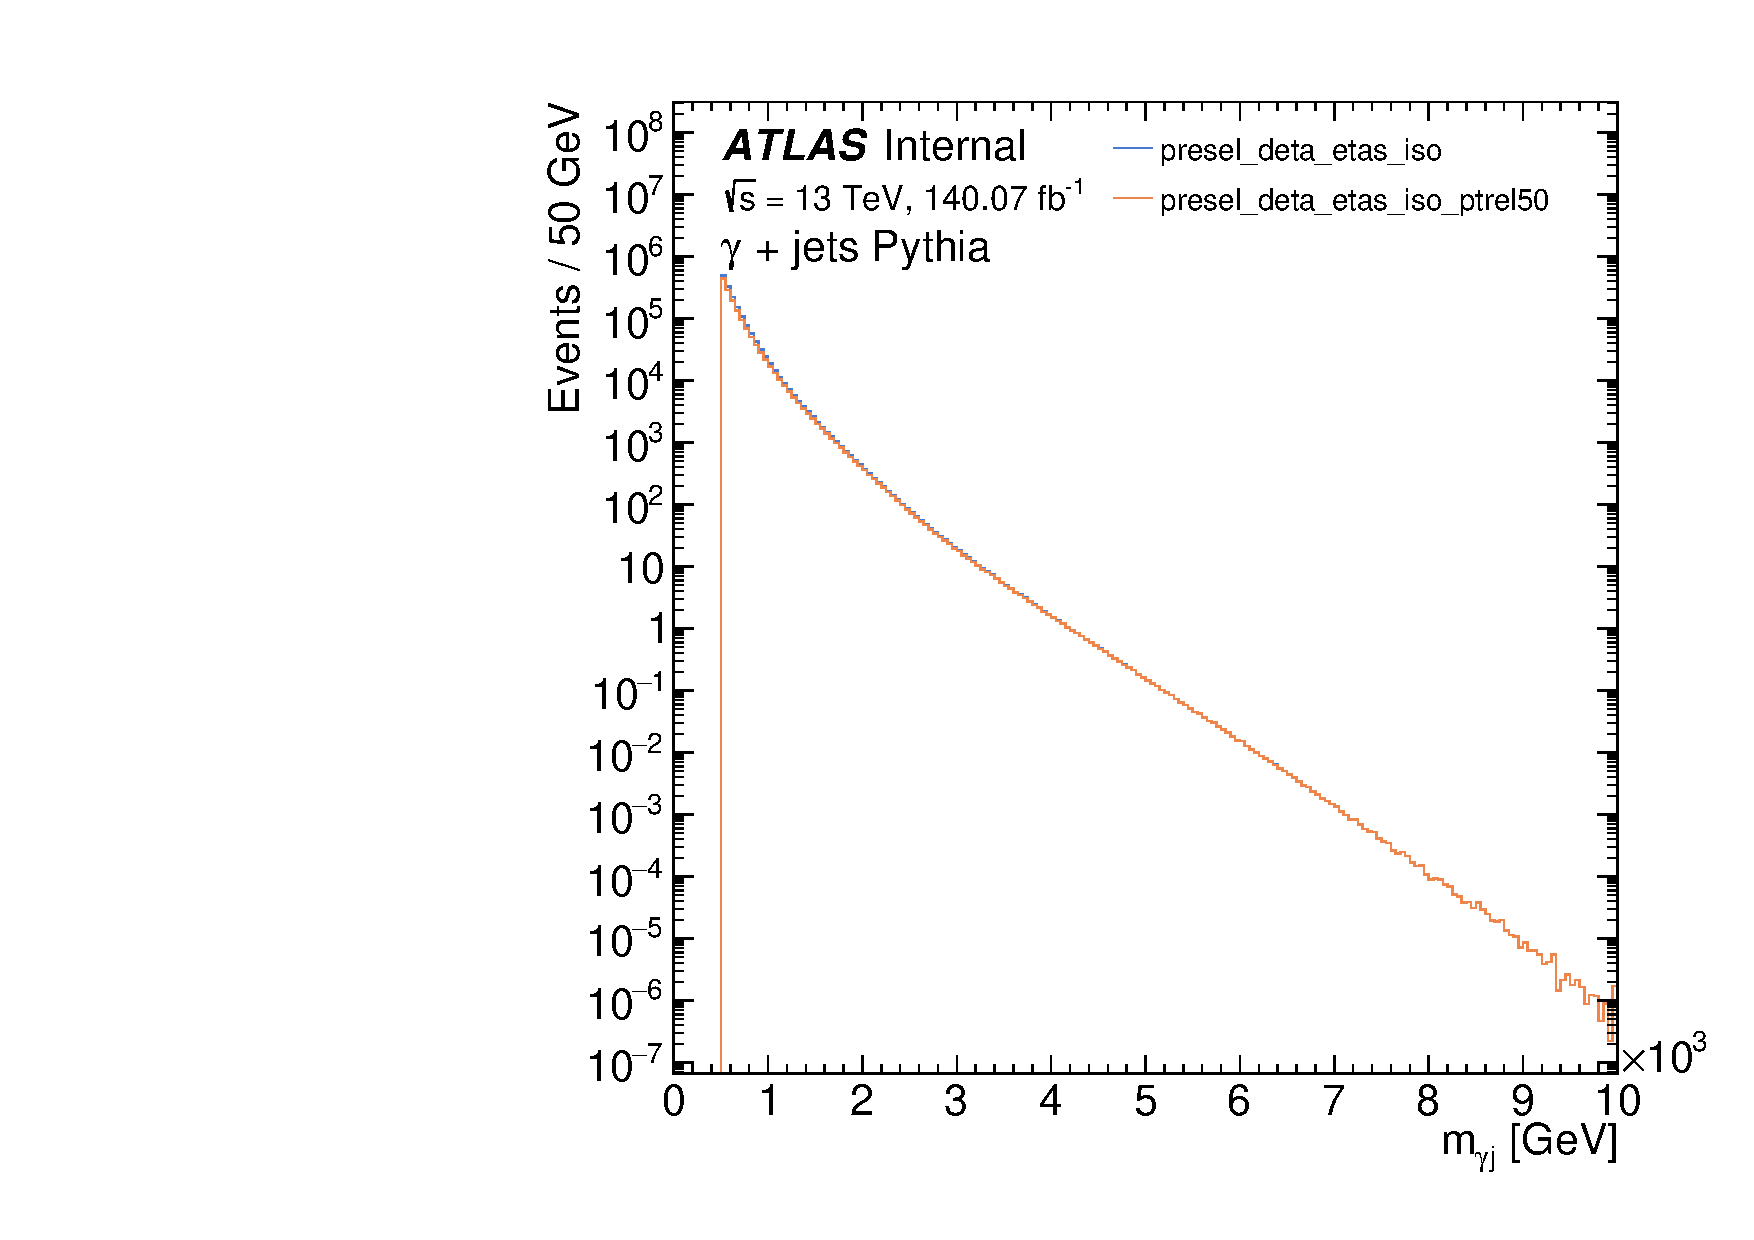
\includegraphics[width=0.45\linewidth]{5_resonances/event_selection/jet_pt/can__photonjet_Pythia__phjet_m__regions_presel_deta_etas_iso_presel_deta_etas_iso_ptrel50__Run2}
    \caption{\myj distribution before and after the \ptjet cut. The orange (blue) line represents the distribution after (before) the cut is applied.}
    \label{fig:evt_selection:sr_opt:jet_pt:phjet_m}
\end{figure}















\section{Signal regions}
\label{sec:evt_selection:sr}


By applying the previously defined cuts (summarised in \Tab{\ref{fig:evt_selection:sr:signal_regions_scheme}}), it is possible to obtain a clean \myj distribution, where the vast majority of fragmentation photon and \(t\)-channel events are removed, but still having high signal efficiency. 

This work will benefit from the further separation that can be achieved by classifying the leading jet into three possible flavours: light-, \(c\)- or \(b\)-tagged jets. Making use of the current \ac{ATLAS} \(b\) and \cjet GN2 tagger, the signal regions SRB SRC and SRL can be defined. A scheme of how this separation occurs is presented in \Fig{\ref{fig:evt_selection:sr:signal_regions_scheme}}. First, \bjets are discriminated against light- and \cjets by menas of the \(77\%\) \btag efficiency \ac{WP}. By selecting those jets that fail to enter region SRB, a \ctagger \ac{WP} of \(50\%\) \ctag efficiency is applied to select \cjets, and those do not pass this \ctagger, are classified as untagged, or, simply \ljets.

\begin{table}[ht!]
    \caption{Signal regions definitions. \fixme{for the moment, all plots have the old naming SRC50/SRL50, but in the text I used SRC/SRL. Should I keep the old naming until I re-do the plots with the correct text?}}
    \label{tab:evt_selection:sr:srs}
    \centering
    \begin{tabular}{|l|>{\centering\arraybackslash}p{0.08\linewidth}|>{\centering\arraybackslash}p{0.08\linewidth}|>{\centering\arraybackslash}p{0.08\linewidth}|>{\centering\arraybackslash}p{0.08\linewidth}|}
        \hline
        Cut                                     & SR & SRB & SRC & SRL \\
        \hline
        \ngamma                                 & \multicolumn{4}{c|}{$>0$} \\ \hline
        \ptgam [GeV]                            & \multicolumn{4}{c|}{$>150$} \\ \hline
        \njet                                   & \multicolumn{4}{c|}{$>0$} \\ \hline
        \ptjet [GeV]                            & \multicolumn{4}{c|}{$>150$} \\ \hline
        \etajet                                 & \multicolumn{4}{c|}{$<1.37 \,\,||\,\, (>1.52 \,\,\&\&\,\, <2.37)$} \\ \hline
        \myj [GeV]                              & \multicolumn{4}{c|}{$>500.$} \\ \hline
        \detayj                                 & \multicolumn{4}{c|}{$<1.6$} \\ \hline
        \etagam                                 & \multicolumn{4}{c|}{$<1.37$} \\ \hline
        \etajet                                 & \multicolumn{4}{c|}{$<1.37$} \\ \hline
        \(\Delta R_{\text{min}} (\gamma, j)\)   & \multicolumn{4}{c|}{$\geq 1.0$} \\ \hline
        \((\ptjet - \ptgam)/\ptgam\)            & \multicolumn{4}{c|}{$<0.5$} \\ \hline
        \btag \(77\%\)                          & - & Pass   & \multicolumn{2}{c|}{Fail} \\ \hline
        \ctag \(50\%\)                          & - & -      & Pass & Fail \\ \hline
    \end{tabular}
\end{table}

\begin{figure}[ht!]
    \centering
    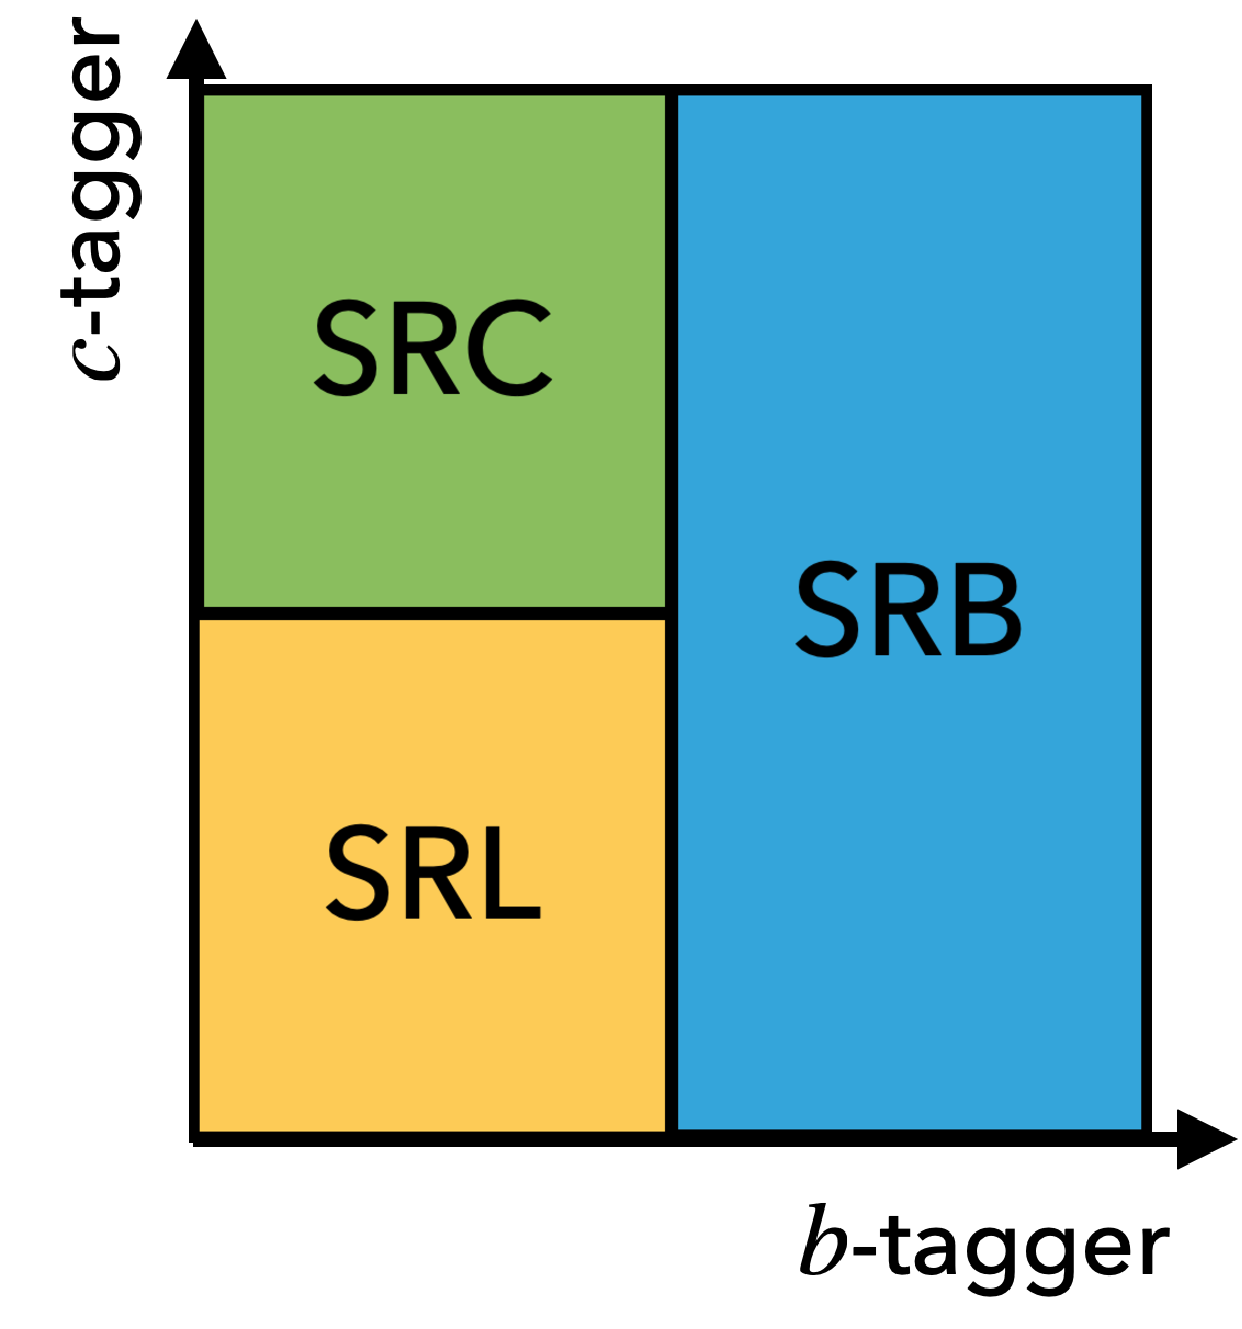
\includegraphics[width=0.35\linewidth]{5_resonances/event_selection/SRL_SRC_SRB-crop}
    \caption{Two-dimensional sequential tagger scheme.}
    \label{fig:evt_selection:sr:signal_regions_scheme}
\end{figure}